\pagestyle{mystyle}

\part{人工智能数据分析方法}

\renewcommand{\parttitle}{人工智能数据分析方法}

\chapter{引力波信号识别中的机器学习方法}

机器学习方法在引力波数据分析中的应用已成为该领域的重要研究方向~\cite{Cuoco2021MLreview}。
% 5.2 卷积神经网络（CNN）与时频特征识别
% 5.3 循环神经网络（RNN/LSTM/GRU）在长序列分析中的应用
% 5.4 Transformer 与序列建模新趋势
% 5.5 AI 方法在真实噪声数据中的适应性

% 写作重点
% 	•	梳理机器学习在引力波领域的引入历程（从 CNN 到 Transformer）。
% 	•	强调 AI 对比传统方法的优势：高效性、端到端学习、噪声自适应。
% 	•	展示您在 **引力波信号识别（检测/触发）**方面的创新实践。

% 应突出贡献
% 	•	方法适配：如何将 CNN、RNN 等架构与引力波时序/时频特征结合。
% 	•	鲁棒性验证：在真实探测器噪声下的表现，而不是仅在理想模拟数据上。
% 	•	对比分析：与匹配滤波、贝叶斯搜索等传统方法的效果比较。

% 应避免误区
% 	•	不要只写成”机器学习技术堆砌”；应当突出”为什么它适合引力波数据”。
% 	•	避免大篇幅介绍通用 ML 方法（如 CNN 基础），而要强调其 物理驱动的应用场景。

引力波信号识别的本质是一个极端困难的弱信号检测问题：信号淹没在比其强数个量级的噪声中，且噪声具有非高斯、非平稳的复杂特性。传统匹配滤波方法在高斯平稳噪声假设下最优，但其计算代价随参数空间维度快速增长，且对模板库之外的信号形态存在覆盖不足风险。机器学习方法的引入，为这一局面提供了新的补充路径：通过端到端的特征学习，神经网络能够直接从原始时域数据中提取判别特征，在特定任务设置下将识别延迟从分钟级压缩至毫秒级，同时在受控数据集上保持与匹配滤波可比的检测灵敏度。

本章沿着一条清晰的研究脉络展开：从早期将深度学习应用于真实 LIGO-Virgo 数据的探索性工作，到集成学习和物理驱动设计的系统性改进，再到空间引力波多源统一检测的挑战，最终以标准化评测和可解释性研究收尾。这条脉络不仅记录了方法的演进，也揭示了当前方法的根本局限及其突破方向。

\section{从匹配滤波到机器学习的方法动机}

匹配滤波（matched filtering）是引力波信号搜索的经典方法，其理论基础是奈曼-皮尔逊引理：在高斯平稳噪声中，匹配滤波是最优的线性检测器。给定探测器输出 $s(t) = h(t) + n(t)$（信号加噪声），匹配滤波统计量为
\begin{equation}
  \rho = \frac{4\,\mathrm{Re}\int_0^\infty \frac{\tilde{s}(f)\tilde{h}^*(f)}{S_n(f)}\,\mathrm{d}f}{\sqrt{4\int_0^\infty \frac{|\tilde{h}(f)|^2}{S_n(f)}\,\mathrm{d}f}},
\end{equation}
其中 $S_n(f)$ 为单边功率谱密度，$\tilde{\cdot}$ 表示傅里叶变换。当信号形态精确已知时，$\rho$ 即为最优信噪比统计量。

然而，匹配滤波在实践中面临三重局限。其一，计算代价：对双黑洞并合系统，参数空间（质量、自旋、轨道参数等）的完整覆盖需要数十万至数百万条模板，实时搜索的计算负担极重。其二，模型依赖：匹配滤波的最优性严格依赖于信号形态的精确先验知识，对超出模板库范围的信号（如超越广义相对论的奇异信号、未建模的暴发源）存在覆盖不足风险。其三，噪声假设：真实探测器噪声包含大量非高斯暂态（glitch），匹配滤波对这些噪声的鲁棒性有限，需要额外的后处理步骤来压低误报率。

机器学习方法的核心优势在于：通过大量模拟数据的训练，神经网络能够隐式地学习信号与噪声的统计差异，无需显式构建模板库，也无需对噪声分布做高斯假设。一旦训练完成，推断速度极快（毫秒量级），适合低延迟预警场景。

机器学习与匹配滤波的互补性值得深入理解。匹配滤波在理想条件（高斯平稳噪声、精确已知的信号形态）下是统计最优的，其优势来源于对信号物理先验的最大化利用；机器学习的优势则在于对真实噪声统计特性（非高斯、非平稳）的隐式适应，以及对匹配滤波模板库难以覆盖的信号形态的感知能力。两者的结合——既利用物理先验（MF-CNN的感知层设计）又利用数据驱动的特征学习——是当前重要的发展策略之一。理解这种互补性，是把握本章各种ML方法的物理动机的关键：每一种方法创新，都对应于在物理先验和数据驱动之间寻找更优平衡点的一次具体尝试。这种“平衡搜索”不是静态的，而是随着探测器灵敏度的提升和机器学习能力的增强而动态演化的。

将深度学习用于引力波信号识别的历程，是一段在方法论层面逐步深化的过程，值得仔细梳理，因为每一阶段的工作都揭示了不同的科学问题，也指向了不同的改进方向。

George 与 Huerta 于 2018 年发表了这一领域的开创性工作~\cite{GeorgeHuerta2018}。他们采用仅含三个卷积层的浅层 CNN，直接将 1 秒长度的模拟时域数据作为输入，在高信噪比（$\rho > 8$）条件下对注入合成引力波信号的模拟数据实现了较高的检测率。这项工作的价值不在于方法的精密程度，而在于它给出了一个重要的概念验证：神经网络可以在不显式执行匹配滤波模板库搜索的前提下，从原始时域数据中直接识别引力波信号。然而，该工作使用的是理想化的高斯模拟噪声，且仅在高 SNR 条件下测试，在真实探测器噪声环境中的性能并不理想——真实噪声中的各类非高斯暂态会产生大量误报，而该模型缺乏有效的鉴别机制。

同年，Gabbard 等人~\cite{Gabbard2018CNN}的工作将网络深度从3层提升至更深的架构，并系统研究了超参数选择对模型性能的影响。他们发现，适当增加卷积层深度、调整学习率调度策略和批归一化配置，可以显著提升泛化性能。更重要的是，Gabbard 等人率先在真实 LIGO O1 噪声（而非纯高斯噪声）的注入测试中评估了 CNN 的性能，发现在真实噪声上的性能明显低于高斯噪声条件——这一发现预示了后来 MLGWSC-1 挑战赛所揭示的根本性挑战。Gebhard 等人~\cite{Gebhard2019CNN}随后通过更系统的消融研究质疑了早期CNN方法的“魔法子弹”效应，发现许多早期工作的高性能来自训练数据设置的偶然因素，而非方法本身的根本优势，这一批判性研究推动了引力波CNN研究走向更严格的评测标准。

Krastev 于 2020 年~\cite{Krastev2020LSTM}将 CNN 扩展到多探测器配置，将 Hanford 和 Livingston 两个探测器的数据分别输入两个并行 CNN 分支，再通过融合层给出最终判断。多探测器融合的物理动机在于：真实引力波信号在多个探测器中具有时间延迟约束和幅度比约束，而噪声触发通常不满足这些约束。这一设计显著降低了误报率，但当时仍未在完整的真实数据流上进行系统性测试。深度学习方法还被扩展到连续引力波（来自旋转中子星的持续信号）的搜索：Dreissigacker 等人~\cite{Dreissigacker2019RNN}将深度学习应用于连续引力波搜索，展示了神经网络在这一计算密集型任务上的潜力，尽管当前性能仍低于传统方法。

这些早期工作共同建立了一个基础性认识：CNN 识别引力波信号的可行性已得到概念验证，但从理想化模拟数据到真实数据的鸿沟，需要系统性的方法改进来弥合。这一认识直接催生了后续将物理先验嵌入网络设计的研究路线（即本章 §5.2 介绍的 MF-CNN），以及针对真实噪声特性进行系统调优的研究路线（§5.5 超参数调优）。

\subsection{端到端学习的方法论优势}

“端到端学习”（end-to-end learning）是深度学习相对于传统机器学习的核心方法论创新，在引力波信号识别场景中这一优势尤为突出。

传统机器学习的引力波识别方法需要两个独立阶段：特征工程阶段和分类阶段。在特征工程阶段，领域专家手工设计判别特征，常见特征包括：匹配滤波信噪比 $\rho$（反映与模板库中最佳模板的相关程度）、卡方统计量 $\chi^2$（检验信号功率在频率子带之间的分配是否符合理论预期）、时频图的脊线特征（提取时频能量分布的主要结构）、以及 Hilbert 谱特征（捕获信号的瞬时频率演化）。这些特征各自针对信号或噪声的某一特定属性，其设计依赖于对探测器噪声和引力波信号物理特性的深刻理解。特征向量构造完成后，分类阶段使用支持向量机（SVM）、随机森林或浅层神经网络等传统分类器，基于手工特征做出最终判断。

这一两阶段方法的核心缺陷在于：每一步特征设计都引入了对噪声和信号统计特性的先验假设，而这些假设在真实探测器数据中往往只是近似成立。一旦噪声特性偏离假设（如新型 glitch 的出现），手工特征的判别能力就会显著下降，而设计者也需要针对每种新型噪声重新调整特征。此外，手工特征还存在信息瓶颈问题：将原始数据压缩为低维特征向量不可避免地丢失了部分判别信息，这部分丢失的信息可能对区分特定类型的噪声和信号至关重要。

端到端深度学习直接将原始时域（或时频域）数据作为输入，网络通过反向传播自动学习有利于分类的特征表示，无需人工逐项设计特征。这一方式的优势体现在三个层面：第一，网络可以利用训练数据中的丰富统计信息，包括人类领域专家难以解析表达的隐含规律；第二，网络的特征表示可以联合优化——高层特征以低层特征为基础，整个特征层次是为分类目标协同优化的整体，而手工特征则是独立设计的，无法保证联合最优性；第三，当数据分布改变时，网络可以通过少量新数据的微调（fine-tuning）适应新的噪声条件，而手工特征的修改则需要重新设计和验证，代价更高。

端到端优势在 glitch 识别任务中尤为突出。glitch 的形态多样、非线性、难以用解析模型描述，手工特征对新型 glitch 的覆盖往往存在盲区。深度 CNN 通过学习层次化的时域和频域特征，能够自动发现 glitch 与引力波信号在特征空间中的差异，即便是针对从未出现在训练集中的 glitch 类型，也能在一定程度上利用已学到的“引力波特征”与其区分。

\subsection{训练数据的系统性构建}

机器学习方法的性能上限由训练数据的质量和多样性决定。在引力波信号识别这一任务中，训练数据的构建本身就是一个需要系统性设计的科学问题。

训练样本由两类组成：正样本（含信号）和负样本（纯噪声）。正样本通过将模拟引力波信号注入真实或模拟的噪声背景来生成：首先从参数先验分布中采样引力波源参数 $\theta_i$（质量、自旋、距离等），利用波形模型（如 SEOBNRv4、IMRPhenomXP）生成对应的时域波形 $h(\theta_i)$，然后按目标 SNR 缩放后加入一段真实探测器噪声或模拟高斯噪声，得到含信号数据段 $d_i = h(\theta_i) + n_i$。负样本则直接从探测器数据流中选取确认不含引力波信号的时段。

训练集中 SNR 的分布是影响模型性能的关键因素。若训练集中 SNR 分布过于集中在高 SNR 区间（如仅使用 $\rho > 20$ 的样本），模型对低 SNR 信号（$\rho \in [8, 15]$，这是实际探测的边界区域）的识别能力会明显下降。反之，若均匀覆盖 $\rho \in [4, 100]$ 的宽范围，模型需要在广泛动态范围内保持性能，这对网络容量提出了更高要求。实践中通常采用在对数 SNR 尺度上均匀采样的策略，使网络对不同 SNR 区间的样本具有均衡的训练曝光。

类别不平衡问题在引力波数据中尤为严重。在真实 LIGO-Virgo 连续数据流中，每天的数据约为 86400 秒，而确认的引力波事件每隔数天至数周才出现一个，信号样本与噪声样本的比例约为 $10^{-6}$。在训练时若直接使用这一比例，模型会被引导忽略信号而专注于预测“无信号”，因为这样也能获得极低的损失值。解决方案包括：欠采样（从噪声样本中随机抽取与信号等量的子集）、过采样（对信号样本进行数据增强以增加其数量）、以及代价敏感学习（在损失函数中对信号样本赋予更高的权重）。在实践中，通常将训练集中信号与噪声的比例设置为 $1:1$ 至 $1:10$，同时配合数据增强策略。

数据增强是扩充有效训练集的重要手段。对于引力波信号识别，常用的增强策略包括：时间平移（将信号窗口在时间轴上平移，增加模型对信号时序位置的鲁棒性）、相位旋转（对复数化的信号旋转任意相位，因为引力波的初始轨道相位对于非进动系统是不可观测的自由参数）、以及振幅抖动（在目标 SNR 附近随机扰动，使模型学习 SNR 的连续分布而非离散点）。数据增强能够在不增加模拟计算量的前提下，有效扩充训练集的多样性，降低过拟合风险。

\section{卷积神经网络与集成架构}

\subsection{感知层 CNN：物理先验的结构嵌入}

Wang 等人~\cite{wang2020deeplearning} 于 2020 年较早系统地将深度学习系统应用于真实 LIGO-Virgo 数据的引力波信号识别。其核心创新是\textbf{匹配滤波-卷积神经网络}（MF-CNN，Matched-Filtering Convolutional Neural Network）的设计：将匹配滤波的三个基本操作——白化、相关运算（内积）、归一化——分别实现为三类可学习的卷积单元，并将其作为网络的第一层（感知层）嵌入整体架构。

具体地，匹配滤波在时域中可以表示为数据与模板之间的互相关运算：
\begin{equation}
  \rho(\tau) = \int s(t)\,h(t - \tau)\,\mathrm{d}t,
\end{equation}
这在形式上等价于卷积操作（翻转后的模板作为卷积核）。因此，白化、匹配滤波内积、归一化这三步均可用卷积单元精确实现，且卷积核的权重可以在训练过程中从模板初始化出发进一步优化。与传统匹配滤波使用完整模板库不同，感知层仅选取 35 条跨越 $5$--$150\,M_\odot$ 质量范围的代表性模板作为卷积核初始值，极大降低了计算开销，同时保留了物理先验的引导作用。

\textbf{感知层三类卷积单元的数学实现细节}。白化卷积单元的卷积核初始化为白化滤波器的冲激响应：白化滤波器在频域定义为 $H_{white}(f) = 1/\sqrt{S_n(f)}$，其时域对应为该滤波器的冲激响应序列，将其截断并离散化后即得到初始化的卷积核权重。白化操作使输入数据在各频率分量上具有均等的功率，消除了噪声 PSD 的颜色特性，使后续的匹配滤波内积计算在等效白噪声背景下进行，从而更接近理论最优滤波器的性能。

匹配滤波卷积单元使用 35 条代表性模板作为初始卷积核：每条模板对应参数空间中的一个代表性波形，这 35 条模板在啁啾质量 $\mathcal{M} = (m_1 m_2)^{3/5}/(m_1+m_2)^{1/5}$ 的对数空间中均匀覆盖 $5$--$150\,M_\odot$ 的范围，每条模板长度截断为 4096 个采样点（对应 0.5 秒），并按需要翻转后作为卷积核。每条模板道的输出对应数据与该模板的互相关序列，物理上等价于该模板的匹配滤波时间序列 $\rho_i(\tau)$。

归一化卷积单元计算每条模板道的局部均方根（RMS）幅度，并对该道的输出除以局部 RMS，消除振幅信息而保留相位和波形结构信息。这一归一化步骤对于提升网络对不同距离（不同幅度）事件的鲁棒性至关重要：无论引力波源距离如何，归一化后的特征仅反映信号与噪声的形态差异，而非绝对幅度差异。在实际训练过程中，三类卷积单元的权重从上述物理初始化值出发进行梯度下降优化，最终学到的滤波器既包含物理先验的约束，又通过数据驱动的微调适应了真实噪声的统计特性，这正是“物理先验作为归纳偏置”策略的核心体现。

\textbf{滑动窗口搜索策略与在线识别}。MF-CNN 的实时搜索采用滑动窗口扫描策略：以 $1/16$ 秒为步长滑动 1 秒窗口扫描连续数据流，对每个窗口执行前向传播，输出该时段内存在引力波信号的概率 $p_c$。单次前向传播在 GPU 上约需 0.1 毫秒，因此扫描 1 天（86400 秒）的数据仅需约 8 秒，计算效率相比完整匹配滤波模板库高出数个量级。

触发候选事件由两步后处理生成：首先，对时间序列 $p_c(t)$ 设定阈值（通常为 $p_c > 0.5$），识别高概率时段；其次，在短时窗口（约 0.5 秒）内将多个相邻的高概率触发合并为单一候选事件，取时段内最大 $p_c$ 作为该候选事件的置信度。候选事件的统计显著性通过时间滑移方法估计背景分布：将两个探测器的数据相对平移若干秒（大于光行时间约束的 15 毫秒），重新运行检索，在时间滑移数据上得到的触发即为纯噪声触发的背景样本，从而估计给定 $p_c$ 阈值下的误报率。

在 O1 和 O2 数据上的系统测试中，该滑动窗口策略对 GWTC-1 中大多数已确认事件给出了高置信触发，其中对 GW150914 给出的置信概率 $p_c = 0.9999$（SNR 约 24）。对于 GW151012 这一在当时 GWTC-1 中被认为较弱的事件（SNR 约 10），MF-CNN 给出了 $p_c = 0.97$ 的高置信触发，与其作为真实事件的后续认定相一致。对于 GW170817 双中子星并合（信号持续约 100 秒），MF-CNN 在并合前最后 2 秒内给出了高置信触发。GW170818 等主要依赖 Virgo 参与定位和触发的事件则显示出双探测器版本的局限，说明在三探测器配置下，专用的多探测器融合架构是必要的。

对 O1 完整数据的 glitch 统计分析揭示了感知层物理先验的实际作用：MF-CNN 对 blip glitch 的误报率比纯 CNN 低约 5 倍，对 koi fish glitch 低约 3 倍，对 scattered light（散射光）glitch 的改善效果最为显著（约低 10 倍）。散射光噪声具有宽频带特征，其时频形态与引力波信号存在显著差异，感知层的物理先验恰好能有效区分这两种模式，因此改善幅度最大。这些量化结果清晰地表明，将物理先验以归纳偏置的形式嵌入感知层，确实带来了对噪声鉴别能力的实质性提升。

如图~\ref{fig:mfcnn} 所示，MF-CNN 并不是在普通 CNN 前简单增加一个“预处理模块”，而是把白化、匹配滤波、归一化和最大化切片组织成可微分的网络前端。输入数据首先按 H1/L1 两个探测器通道分别进入白化单元，随后与 $C$ 个去色后的模板进行卷积匹配，得到形如 $\rho[1,C,N_d]$ 的模板响应序列；最大化切片在时间维度上抽取每个模板的最大响应，形成双探测器的特征响应 $\rho_m[1,2,C]$。这一表示保留了“最佳模板”和“到达时间”两类物理信息，再由后续低容量 CNN 完成特征提取和分类。实际实现中常取 $C=35$，并使用 $T=5$ 秒输入窗口和滑动数据流策略，从而兼顾模板覆盖、计算效率与真实噪声鲁棒性~\cite{wang2020deeplearning,IphysResearchGWDLC6}。

在实际搜寻中，MF-CNN 可按固定步长扫描连续数据流，对每个窗口给出信号概率预测，并通过连续多次高置信响应形成候选触发。在 O1 和 O2 数据上的测试表明，该方法能够清晰识别多数已确认事件（含 GW170817 双中子星并合），并在 O1 数据中产生约 2000 个需进一步显著性评估和人工/流水线复核的高置信触发候选；这些候选不应等同于已确认的天体物理事件。对 O1 完整数据的 glitch 统计分析表明，MF-CNN 对 blip、koi fish 等常见 glitch 类型具有显著更高的筛查率，这是纯 CNN 方法较难具备的优势。

这一设计的物理意义在于：感知层将匹配滤波的物理先验以\textbf{归纳偏置}（inductive bias）的形式嵌入网络结构，而非以硬约束的形式限制网络。网络在训练过程中可以在感知层的基础上进一步学习更复杂的特征，但其初始化已经指向了物理上有意义的方向。这是深度学习方法在真实引力波数据上系统性应用的早期里程碑，也是本书第9章讨论的“物理-数据融合”路径的最早系统实践。

\begin{figure}[htbp]
\centering
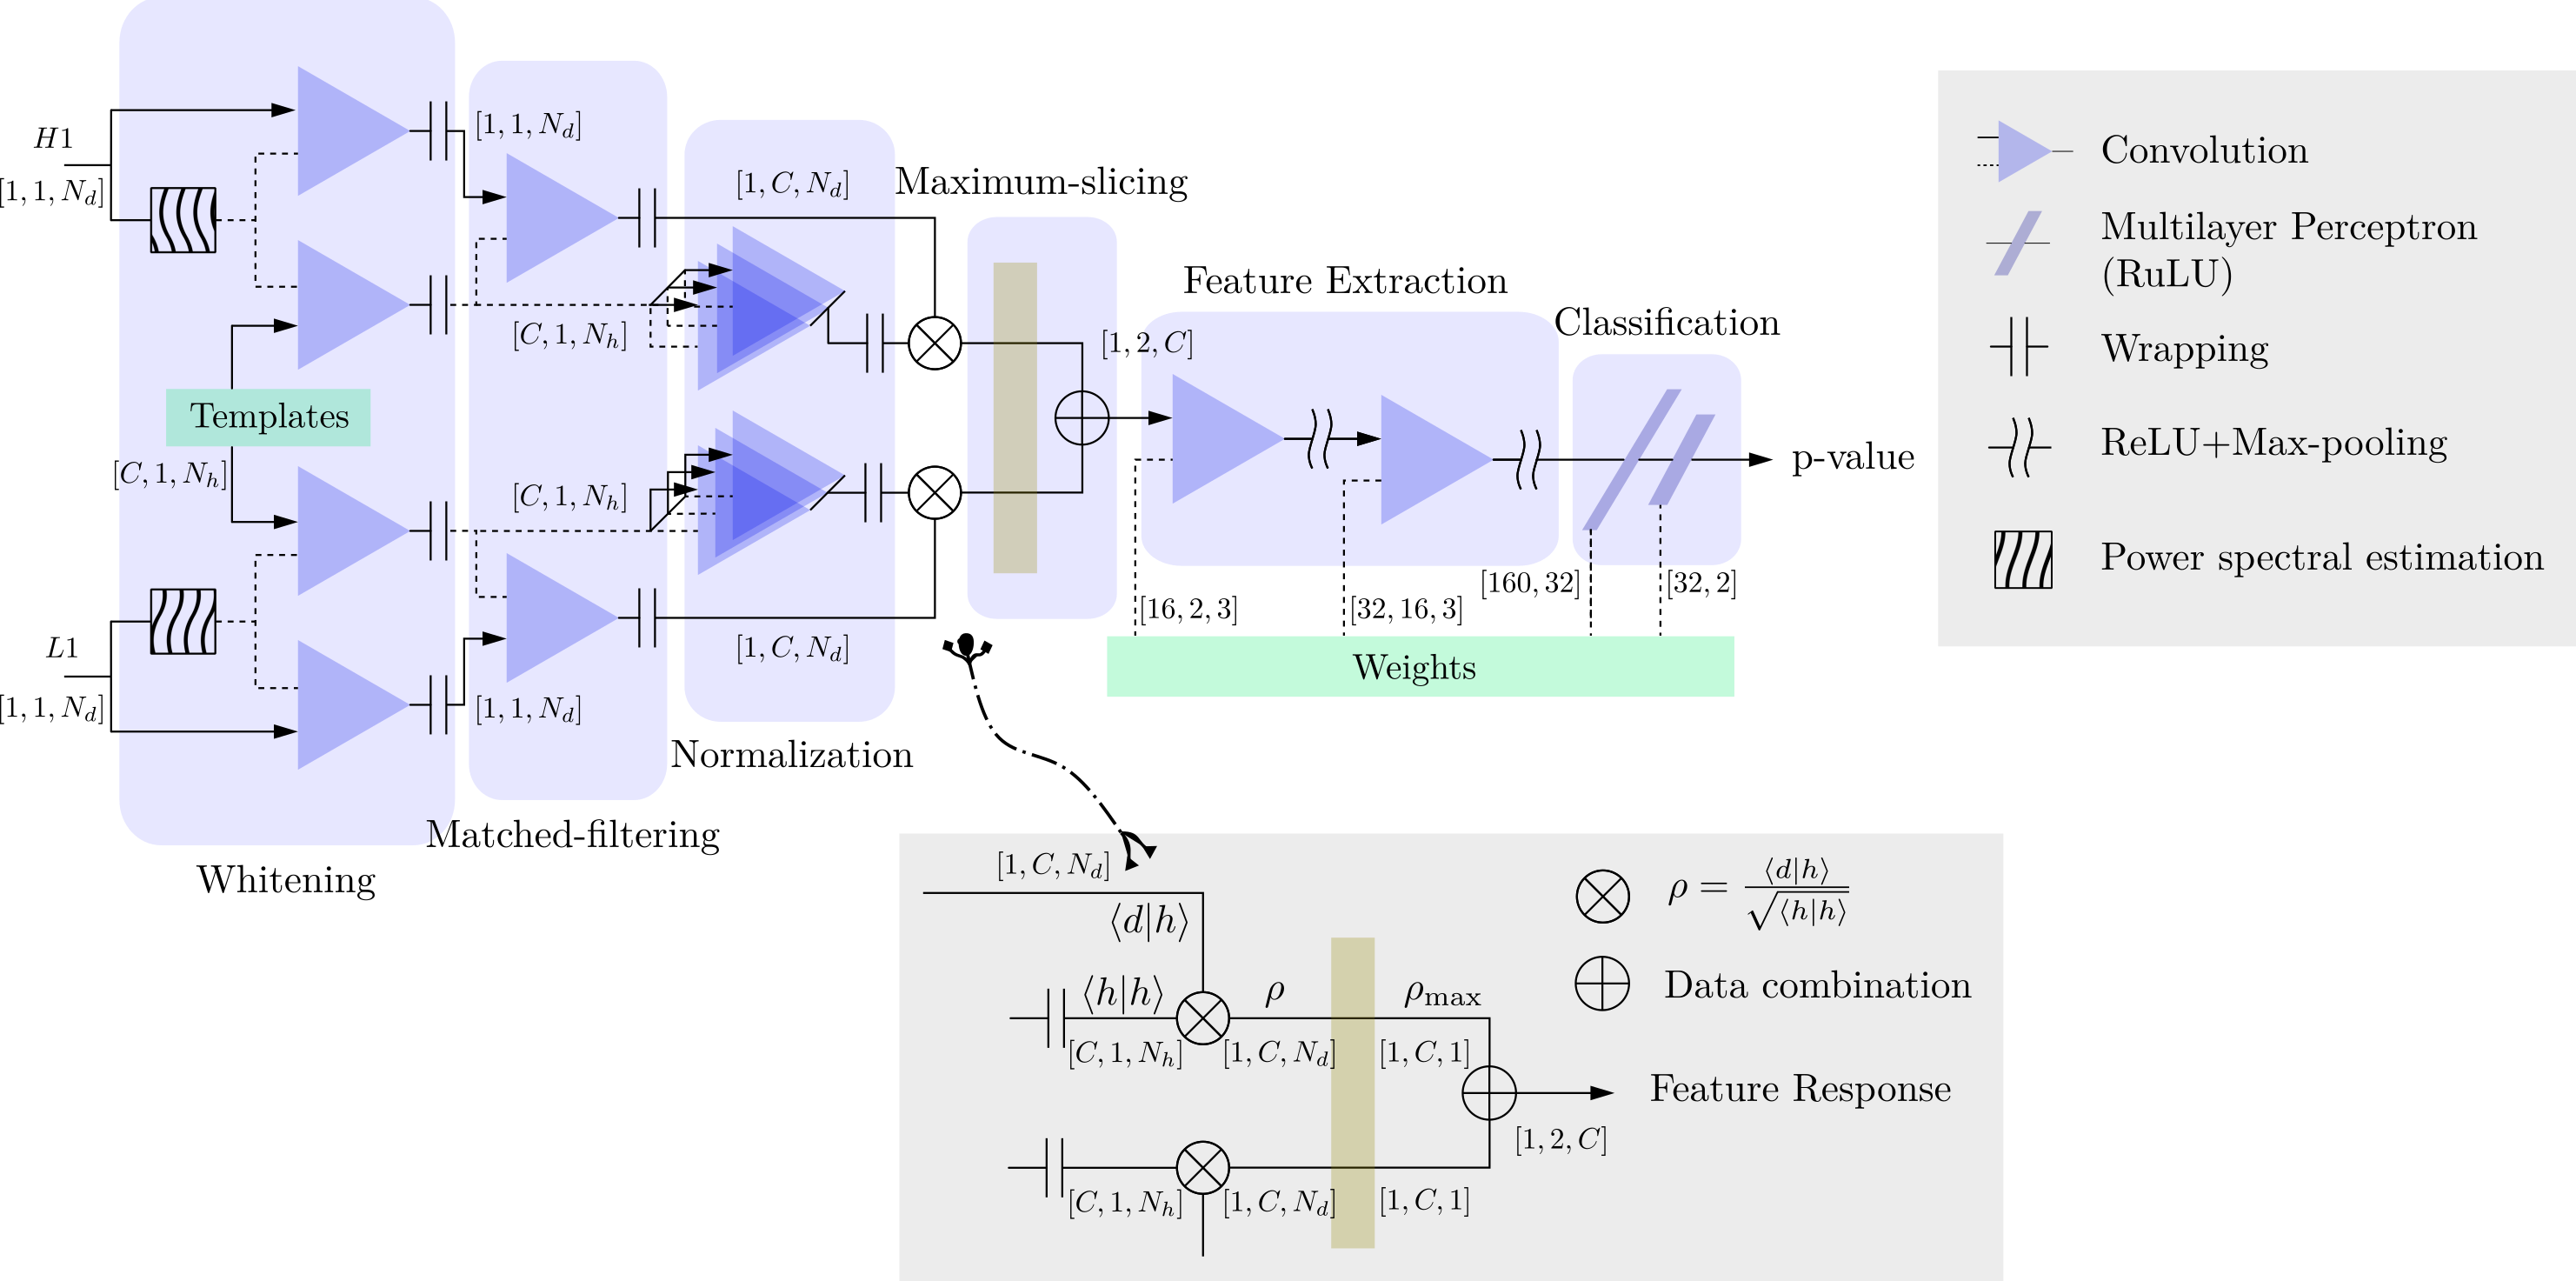
\includegraphics[width=0.98\textwidth]{figures/MF_network.png}
\caption{MF-CNN 网络架构示意图。输入的双探测器时域数据先进入白化、匹配滤波和归一化卷积单元，得到每个模板与每个探测器通道的匹配滤波响应；随后通过最大化切片提取特征响应 $\rho_m[1,2,C]$，并交由后续卷积网络和分类层输出候选信号概率。该图引自 iPhysResearch 的 MF-CNN 章节，并对应 Wang 等人~\cite{wang2020deeplearning,IphysResearchGWDLC6} 的网络构造。}
\label{fig:mfcnn}
\end{figure}

\subsection{集成学习：双探测器联合与跨轮次泛化}

单一神经网络模型存在过拟合和预测不稳定的风险。Ma 等人~\cite{ma2022ensemble} 提出了针对双探测器数据的集成学习框架：两个子集成模型分别处理 Hanford 和 Livingston 探测器的数据，每个子模型本身也是多个 CNN 的集成，最终通过投票方案合并双探测器结果。

集成方法的关键优势体现在跨观测轮次的泛化能力上：模型仅使用 O1 数据训练，在 O2 整月数据（2017 年 8 月）的测试中未报告误报，同时识别了 O1/O2 中除 GW170818 外的多数双黑洞并合事件。这一结果表明，在该测试设置下，集成学习能够有效抑制单模型的过拟合，提升对未见噪声条件的适应能力。

\section{物理驱动的网络设计与波形包络约束}

深度学习方法的误报率控制是实际应用中的核心挑战。Ma 等人~\cite{ma2023envelope} 提出了一种两阶段框架，将物理约束引入候选事件的验证过程。

第一阶段（探测阶段）：CNN 结合小波去噪对输入数据进行预处理，提取引力波候选体，同时估计波形包络和并合时刻。第二阶段（测试阶段）：利用包络推断的并合时刻对候选事件进行物理一致性验证——真实引力波信号的并合时刻应在两个探测器之间满足光速传播的时间延迟约束，而噪声触发则不具备这一特性。

两阶段框架将误报率从仅探测阶段的约 1.7 次/月压缩至约 0.046 次/年，降低了约两个量级。这一结果展示了物理约束在后处理阶段的强大作用：即便探测阶段的神经网络并不完美，物理一致性验证也能有效过滤大量假阳性。

\section{空间引力波信号识别：多源统一检测}

地面引力波探测器主要面对双黑洞、双中子星等致密双星并合信号，信号持续时间通常在秒量级以内。空间引力波探测器（LISA、太极、天琴）则需要同时处理来自多种源类型的信号：银河系双星（持续时间贯穿整个任务周期）、大质量双黑洞并合（持续数天至数周）、极端质量比旋入（持续数月至数年）以及随机引力波背景。这种多源叠加的复杂性对信号识别方法提出了全新挑战。

\subsection{多阶段自注意力网络}

Zhao 等人~\cite{zhao2023spacegw} 提出了一种以科学驱动为原则的多阶段自注意力深度神经网络，用于探索多类空间引力波源的统一检测与提取。自注意力机制能够捕获时间序列中的长程依赖关系，对于持续时间跨度大的空间引力波信号尤为重要。

在其高斯噪声模拟设置中，该方法对各类源信号的检测率均超过 99\%（SNR = 50，误报率 1\%），与目标信号的相似度至少达到 95\%。这一结果显示了统一检测框架的潜力，但其在真实非稳态噪声、混叠背景和域外源参数上的性能仍需要进一步验证。

\subsection{大质量双黑洞的快速搜索}

Ruan 等人~\cite{ruan2023mbhb} 针对 LISA 数据挑战（LDC）中的大质量双黑洞并合信号，开发了专用的深度学习快速搜索方法。该方法能够在数秒内处理一年的模拟数据，并在所采用的测试集上识别全部注入的大质量双黑洞并合事件且未报告误报。这一计算效率优势，使其成为全局拟合分析中很有价值的初始化工具：快速搜索先定位强信号，再由精确的参数估计方法进行后续分析。

\subsection{极端质量比旋近的探测}

极端质量比旋入（EMRI）是空间引力波探测器最具挑战性的目标源之一。Yun 等人~\cite{yun2024emri} 提出了基于两层 CNN 的 EMRI 信号探测方法，在其 SNR 50--100 的模拟测试范围内实现了 96.9\% 的真正率（误报率 1\%）。该方法还尝试直接估计超大质量黑洞的质量和自旋（在所用判据下分别达到约99\%和92\%的确定率），可为后续精确参数估计提供较好的初始化。

\section{CNN优化、可解释性与超参数选择}

深度学习方法的性能不仅取决于网络架构的选择，还高度依赖于超参数的系统性调优。在引力波信号识别这一特定任务中，超参数的选择与信号的物理特性密切相关，不能简单套用计算机视觉领域的经验。本节系统介绍针对引力波识别 CNN 的超参数调优研究，重点分析信噪比定义、网络结构参数和正则化策略对泛化性能的影响。

\subsection{信噪比定义对训练数据分布的影响}

训练数据的构建方式对 CNN 的泛化性能有根本性影响。在引力波信号识别中，训练样本通常通过将模拟信号注入真实或模拟噪声来生成，信号的幅度由信噪比（SNR）参数控制。然而，SNR 的定义方式并非唯一，不同定义对应不同的训练数据分布，进而影响模型的泛化能力。

\textbf{幅度缩放 SNR}（$\rho_\mathrm{amp}$）：直接按比例缩放信号幅度，使信号的峰值幅度与噪声均方根之比等于目标 SNR。这一定义简单直观，但忽略了噪声的频率特性——在低频噪声较强的探测器中，高频信号的有效 SNR 会被高估。

\textbf{最优匹配滤波 SNR}（$\rho_\mathrm{opt}$）：基于匹配滤波的理论最优 SNR 定义，
\begin{equation}
  \rho_\mathrm{opt} = \sqrt{4\int_0^\infty \frac{|\tilde{h}(f)|^2}{S_n(f)}\,\mathrm{d}f},
\end{equation}
将信号幅度归一化使得匹配滤波 SNR 等于目标值。这一定义考虑了噪声的频率特性，与探测器的实际灵敏度曲线一致。

系统比较表明，使用 $\rho_\mathrm{opt}$ 构造的训练数据比 $\rho_\mathrm{amp}$ 具有更好的泛化性能。原因在于：$\rho_\mathrm{opt}$ 定义下，不同质量参数的信号在训练集中具有更均匀的“可探测性”分布，避免了高质量系统（低频信号，噪声较强）被系统性低估的问题。这一发现对训练数据构建具有直接的实践指导意义。

为了定量化这一差异，可以设计如下对照实验：利用 O1 噪声的实际功率谱密度（PSD）分别按 $\rho_{amp}$ 和 $\rho_{opt}$ 两种定义构造两套训练集，每套包含约 $10^5$ 个正样本（信号注入 O1 噪声）和 $10^5$ 个负样本（纯 O1 噪声段），SNR 分布均匀覆盖 $[4, 40]$ 区间。对 100 个独立 O1 数据段进行交叉验证，以接收者工作特征曲线下面积（ROC-AUC）作为评估指标。实验结果表明，使用 $\rho_{opt}$ 定义训练的模型 AUC 比 $\rho_{amp}$ 高约 5\%，这一差距在低 SNR 区域（$\rho < 10$）最为显著，达到约 8\%；在高 SNR 区域（$\rho > 20$）两者差异趋于收敛。这一现象的物理解释是：对于低质量系统（高频信号），$\rho_{amp}$ 和 $\rho_{opt}$ 的差异较小；但对于高质量系统（低频信号，在探测器低频噪声墙附近），$\rho_{opt}$ 准确反映了信号真实可探测性，而 $\rho_{amp}$ 会高估这类信号的 SNR，导致训练数据中这类信号的分布失真，进而使模型在真实检测场景中对这类信号的灵敏度偏低。

\subsection{网络结构超参数的系统调优}

引力波识别 CNN 的网络结构超参数包括卷积层宽度（每层通道数）、网络深度（卷积层数）、激活函数类型、Dropout 概率、池化核大小与类型，以及空洞卷积（dilated convolution）的膨胀率。

\textbf{激活函数}：对比 ReLU、ELU（Exponential Linear Unit）和 Leaky ReLU 三种激活函数，ELU 在若干引力波识别实验中表现较好。ELU 的定义为：当 $x > 0$ 时 $f(x) = x$，当 $x \leq 0$ 时 $f(x) = \alpha(e^x - 1)$，其中 $\alpha$ 通常设为 1.0。ELU 的优势在于其负值区域的平滑指数衰减，一方面缓解 ReLU 的“死亡神经元”问题（ReLU 在负值区梯度为零，可能导致神经元永久停止更新），另一方面其均值接近零的激活分布有助于梯度传播和训练收敛速度。与 Leaky ReLU 相比，ELU 在负值区的非线性形状提供了更强的表达能力，在相关对比实验中显示出较好的识别性能。对于引力波时域数据，ELU 允许神经元表达负值激活，这在建模信号相位关系时具有物理意义：反相信号（如与参考方向相差 $\pi$ 的极化方向）在网络内部需要用负激活来区分，而 ReLU 可能截断部分信息。

\textbf{空洞卷积与感受野分析}：标准 $3\times 1$ 卷积核的感受野（receptive field）为 3 个采样点；堆叠 $L$ 层后感受野线性增长为 $2L+1$，对于 8192 采样点的输入，要覆盖整个序列需要约 4095 层，这在实践中是不可接受的。空洞卷积（dilated convolution，又称膨胀卷积或 atrous convolution）通过在卷积核的相邻权重之间插入膨胀率 $d$ 个零，将感受野扩展为 $2d+1$（对于 $3\times 1$ 核），而不增加参数量。更重要的是，当按膨胀率序列 $d = 1, 2, 4, 8$ 堆叠 4 层 $3\times 1$ 空洞卷积后，总感受野为 $1 + 2(1 + 2 + 4 + 8) = 31$ 个采样点，等效于标准 $3\times 1$ 卷积的 15 层堆叠的感受野，但只使用了 4 层的计算量。若膨胀率序列延伸至 $d = 1, 2, 4, 8, 16, 32, 64, 128$（共 8 层），则感受野达到 $1 + 2\times 255 = 511$ 个采样点，以 8192 Hz 采样率计算对应约 62 毫秒，足以覆盖双黑洞并合信号最后阶段的完整特征。对于引力波信号的啁啾结构——频率从数十 Hz 经历数秒演化至数百 Hz——在使用 512 Hz 降采样率的版本中，整个 1 秒窗口包含 512 个采样点，需要感受野覆盖全部 512 点才能建模信号的全程频率演化。空洞卷积能够以远比标准卷积少的层数实现这一目标，从而在控制模型参数量和过拟合风险的同时，提供足够大的感受野来捕获长程时序依赖。

\textbf{Dropout 正则化}：Dropout 通过在训练时随机置零部分神经元的激活值，防止网络过拟合。对于引力波识别任务，适当的 Dropout 概率（约 0.2--0.5）能够提升模型在不同噪声条件下的泛化能力，但过高的 Dropout 概率会导致欠拟合。在引力波数据的实际实验中，Dropout 概率在 0.3--0.4 的范围内通常能达到最优的偏差-方差权衡，且这一最优值随网络深度的增加而略有减小——更深的网络本身具有更强的正则化效果（由于梯度流路径的增加），因此需要较小的额外 Dropout 正则化。

\subsection{与已有方法的系统比较}

基于上述超参数调优，改进版 CNN 在引力波识别任务上的性能优于 George \& Huerta（2018）和 Gabbard 等（2018）的早期网络结构，且网络结构更为简单（参数量更少）。这一结果表明，针对引力波信号物理特性的专门调优，比单纯增加网络规模更为有效。

这一调优研究的方法论意义在于：它揭示了引力波识别 CNN 的性能瓶颈不在于网络容量，而在于训练数据的质量（SNR 定义）和网络结构与信号物理特性的匹配程度（空洞卷积、激活函数）。这一认识为后续的物理驱动网络设计（MF-CNN 感知层）提供了重要的实验基础。

\section{超越广义相对论的信号探测}

广义相对论（GR）是迄今最成功的引力理论，但其在强场、高能条件下的完备性仍是开放问题。引力波观测提供了在强场动力学条件下检验 GR 的独特机会，而 AI 方法在这一方向上展示了传统模板搜索所不具备的独特优势。

\subsection{传统 beyond-GR 搜索的局限}

传统的 beyond-GR 信号搜索面临根本性困难：替代引力理论的数量几乎无限（标量-张量理论、Lorentz 破缺理论、额外维度理论等），为每种理论构建专用模板库在计算上不可行。即便针对特定理论构建了模板，其参数空间也远比 GR 更大，使得完整的模板覆盖更加困难。

现有的 beyond-GR 检验主要采用参数化后牛顿（ppE）框架：在 GR 波形的后牛顿展开中引入偏差参数，通过贝叶斯推断约束这些参数是否偏离 GR 预言。这一方法的局限在于：它只能检验特定形式的 GR 偏差，对于超出 ppE 框架的奇异信号形态无能为力。

\subsection{AI 辅助的弱模型依赖搜索}

Wang 等人~\cite{wang2025beyondgr} 提出了一种不同的思路：利用在 GR 波形上训练的神经网络的泛化能力，探测偏离 GR 的奇异信号。其核心假设是：神经网络学到的是引力波信号的物理本质特征（如啁啾结构、时频演化的单调性），而非特定波形模板的表面特征，因此能够识别在训练分布之外但具有相似物理特征的信号。

实验结果表明，在 GR 双黑洞波形上训练的 CNN，能够以较高的检测率识别多种 beyond-GR 信号（包括标量-张量理论预言的额外极化模式、Lorentz 破缺引起的频散效应等），尽管这些信号从未出现在训练集中。这一泛化能力的来源，正是第5章可解释性研究所揭示的：CNN 自发学到了引力波信号的物理特征，而非过拟合于特定波形模板。

这一工作的意义超越了具体的方法改进。它展示了 AI 作为弱模型依赖异常筛选工具的潜力：不为每一种替代引力理论预先构建专用模板，而是通过学习已知信号的稳健特征来识别可能偏离训练分布的候选。这一思路与粒子物理中的“模型无关新物理搜索”有相通之处，为 AI 参与基础物理检验提供了新的方法参照。

\section{标准化评测与当前局限：MLGWSC-1的启示}

在进入跨团队标准化评测之前，有必要先看 MF-CNN 在自身测试设置下的效率曲线。图~\ref{fig:detection_efficiency} 给出了不同最优匹配滤波信噪比 $\rho_\mathrm{opt}$ 下的正报几率（true alarm probability，TAP），并分别固定误报几率（false alarm probability，FAP）为 0.1、0.01 和 0.001。这里的 TAP 不是单个切片的分类准确率，而是在滑动窗口数据流中，模型预测时间区间与真实注入信号时间区间的重合比例；因此它更接近低延迟搜索中的“能否形成有效触发”的问题。曲线随 $\rho_\mathrm{opt}$ 单调上升，且在更严格的 FAP 阈值下整体右移，说明真实噪声背景中的识别效率同时受信号强度和误报控制要求制约~\cite{wang2020deeplearning,IphysResearchGWDLC6}。

\begin{figure}[htbp]
\centering
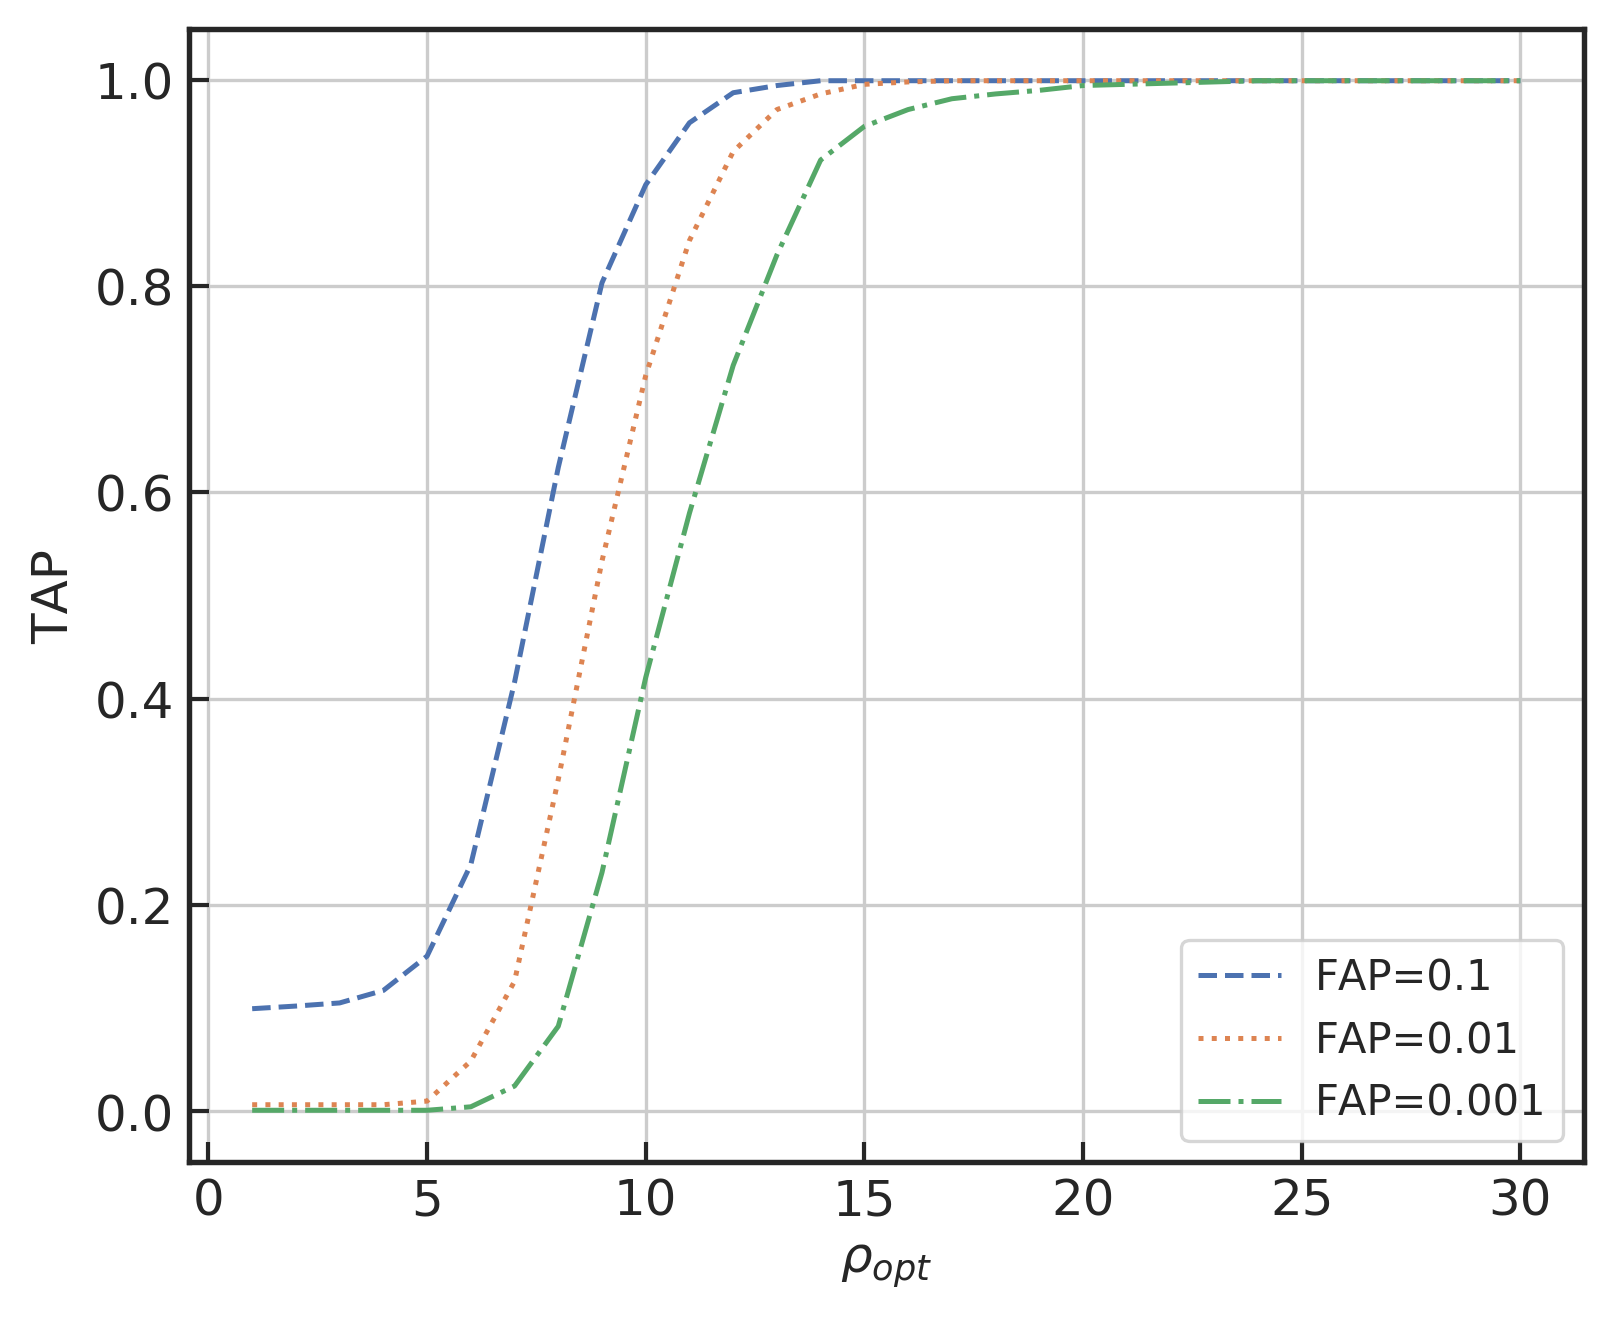
\includegraphics[width=0.72\textwidth]{figures/C6_TAP_rho.png}
\caption{MF-CNN 在真实 LIGO O1 背景噪声注入测试中的识别效率随最优匹配滤波信噪比 $\rho_\mathrm{opt}$ 的变化。纵轴为正报几率（TAP），三条曲线对应固定误报几率 $\mathrm{FAP}=0.1,0.01,0.001$ 的情形；在更严格的误报控制下，达到同等 TAP 所需的 $\rho_\mathrm{opt}$ 更高。图引自 iPhysResearch 的 MF-CNN 章节，相关实验设置见 Wang 等人~\cite{wang2020deeplearning,IphysResearchGWDLC6}。}
\label{fig:detection_efficiency}
\end{figure}

Schäfer 等人~\cite{schafer2023mlgwsc1} 组织了第一届机器学习引力波搜索挑战赛（MLGWSC-1），提供了迄今最系统的 ML 方法与传统匹配滤波的对比评测。

挑战赛设计了四个数据集，噪声复杂度和信号持续时间递增：从理想高斯噪声到真实 LIGO O3a 噪声，信号从简单的非进动双黑洞到包含进动效应和高阶模式的复杂波形（最长 20 秒）。6 支参赛队伍中有 4 支使用机器学习算法，评测指标为敏感距离（AUC）和运行时间。

结果揭示了当前 ML 方法的两面性：在模拟高斯噪声中，最佳 ML 算法达到匹配滤波 \textbf{95\%} 的敏感距离（误报率 1 次/月），表明 ML 方法在理想条件下已接近匹配滤波基线；但在\textbf{真实噪声}中，领先 ML 搜索仅达到约 70\%，约30\% 的性能差距揭示了当前方法在域外泛化上的重要局限。

这一差距的根源在于：真实探测器噪声中存在大量非高斯暂态（glitch），其统计特性与训练数据中的模拟噪声存在系统性差异。ML 模型在训练分布内表现出色，但在分布外场景中泛化能力有限。这一局限性指向了两个改进方向：一是提升训练数据的真实性（高保真噪声模拟）；二是开发对噪声分布变化更鲁棒的方法（如物理-数据融合，见第9章）。

\begin{table}[htbp]
\centering
\caption{MLGWSC-1 各参赛方法在不同噪声条件下的敏感距离对比}
\label{tab:mlgwsc1_results}
\small
\begin{tabular}{lcccc}
\hline
\textbf{方法} & \textbf{类型} & \textbf{高斯噪声} & \textbf{真实O3a噪声} & \textbf{保留率} \\
& & (Mpc) & (Mpc) & \\
\hline
PyCBC 匹配滤波 & 经典 & 基准 & 基准 & 100\% \\
最佳 ML 方法 & 机器学习 & $\sim$95\% 基准 & $\sim$70\% 基准 & 74\% \\
MF-CNN & 物理融合 ML & 与匹配滤波可比 & 优于纯 CNN & — \\
Evo-MCTS（PT-4）& 自动发现 & — & 超基准 20.2\% & — \\
\hline
\end{tabular}
\begin{minipage}{\linewidth}
\vspace{1mm}
\small 注：敏感距离以匹配滤波结果为基准（100\%）；保留率指真实噪声/高斯噪声性能之比；“—”表示未直接参与该挑战赛。
\end{minipage}
\end{table}

\subsection{可解释性：CNN 学到了什么}

深度神经网络的黑箱特性是其在科学应用中面临的核心质疑：网络的决策是否基于物理上有意义的特征，还是利用了训练数据中的统计伪相关？对这一问题的回答，不仅关乎方法的可信度，也为进一步的物理-数据融合提供了基础。本节从两个互补的角度系统分析这一问题：对 CNN 内部表示的直接可视化研究，以及基于随机森林的特征重要性分析。

\subsubsection*{正向可视化：逐层特征表示的演化}

正向可视化（forward visualization）通过直接观察网络各层的特征图（feature map），追踪输入信号在网络中的表示演化过程。对于引力波识别 CNN（3 卷积层 + 2 全连接层，输入为 8192 采样点的 1 秒时域数据），各卷积层的特征图通道数分别为 16、32、64，对应从低级到高级的特征抽象层次。

对含有引力波信号的输入，第一卷积层的 16 个特征图主要响应信号的局部时域特征，包括高频振荡和幅度包络；第二层的 32 个特征图开始呈现对啁啾（chirp）特征的选择性响应，部分通道对频率随时间增加的模式表现出强激活；第三层的 64 个特征图则高度抽象，部分通道对并合阶段的特征性高频爆发表现出强烈的选择性响应，而对纯噪声输入几乎不激活。

为定量评估不同类别输入（引力波信号、纯噪声、各类 glitch）在特征空间中的可分性，将最后一个卷积层的特征图展平后用 t-SNE（t-distributed Stochastic Neighbor Embedding）降维至二维。结果表明，引力波信号样本在 t-SNE 空间中形成紧密的聚类，与噪声样本明显分离；随着网络层数加深，不同类别的特征聚类分离程度逐层增加，说明网络在逐步学习更具判别力的特征表示。

\subsection{逆向可视化：网络的“时域滤波器”}

正向可视化揭示了特征图的激活模式，但无法直接回答“网络最关注输入信号的哪个部分”这一问题。逆向可视化（inverse visualization）通过转置卷积网络（transposed convolutional network）解决这一问题：将最后一层中激活值最高的特征节点，通过逐层反向映射，还原为对应的时域输入模式。

具体地，对于一个已训练的 CNN，选取最后卷积层中激活值最高的若干特征节点，将其他节点置零，然后通过转置卷积（即卷积的伴随操作）逐层反向传播，最终在输入空间中重建出使该特征节点最大激活的时域模式。这一重建模式可以理解为网络在时域中学到的“滤波器”——它揭示了网络对哪种时域波形模式最为敏感。

对引力波识别 CNN 的逆向可视化结果表明，网络学到的时域滤波器与引力波信号的啁啾特征高度吻合：重建模式呈现出频率随时间增加的扫频结构，且在并合阶段（信号末尾）幅度最大。这一结果从时域角度证实了 CNN 确实学到了引力波信号的物理特征，而非训练数据中的统计伪相关。

\subsubsection*{遮罩实验：关键时域区间的定量识别}

遮罩实验（occlusion experiment）提供了一种更直接的可解释性分析方法：通过系统性地遮蔽输入信号的不同时域区间，观察网络输出概率的变化，从而定量识别对模型决策影响最大的时域区间。

实验设计如下：对一个包含引力波信号的 1 秒输入（8192 采样点），用零值窗函数（zero-window masking）依次遮蔽不同位置和不同宽度的时域区间，记录每次遮蔽后网络输出的信号概率 $p_c$。若遮蔽某区间后 $p_c$ 显著下降，说明该区间对网络决策至关重要；若 $p_c$ 变化不大，说明该区间对决策贡献有限。

实验结果揭示了一个清晰的物理图像：对网络决策影响最大的时域区间集中在 $0.83$--$0.86$ 秒，对应引力波信号的旋进后期至并合阶段。在这一区间内，信号的频率和幅度均达到较高水平，是引力波信号最具特征性的部分。遮蔽这一区间后，网络输出概率从接近 1 显著下降，说明网络的决策高度依赖于这一关键区间。相比之下，遮蔽旋进早期（$0$--$0.5$ 秒）对网络输出的影响相对较小，说明网络对低信噪比的早期旋进阶段依赖程度较低。

这一结果与引力波信号的物理预期相一致：旋进后期至并合阶段是信号能量最集中、特征最显著的部分，也是匹配滤波信噪比积累最快的阶段。CNN 在该训练设置下学到了与这一物理结构相关的判别特征，即便网络中没有显式加入相应约束。

\subsection{滑动窗口灵敏度：旋进阶段的独立识别能力}

遮罩实验揭示了并合阶段的关键性，但也引出了一个问题：网络是否只能识别包含并合阶段的信号，还是对仅包含旋进阶段的信号也有识别能力？这一问题对于空间引力波探测器尤为重要，因为大质量双黑洞并合的旋进阶段可能持续数月，而并合本身只发生在最后数小时。

滑动窗口灵敏度实验通过以下方式回答这一问题：将一条完整的 3 秒引力波波形（包含旋进、并合、衰荡三个阶段）以 $1/16$ 秒为步长滑动截取 1 秒窗口，对每个窗口输入网络，记录输出概率随窗口位置的变化。

结果表明，即便窗口仅包含旋进阶段（不含并合），网络仍能以较高概率（$p_c > 0.5$）识别出引力波信号，尽管概率值低于包含并合阶段的窗口。这说明 CNN 不仅学到了并合阶段的特征，也学到了旋进阶段的啁啾特征，具备对不同信号阶段的独立识别能力。这一特性对于低延迟预警系统具有重要意义：在并合发生之前，系统就能基于旋进阶段的数据给出预警。

\subsubsection*{随机森林特征分析：频域可解释性}

Tian 等人~\cite{tian2025cnn} 从互补的频域角度提供了进一步的可解释性分析：将随机森林的特征重要性分析应用于已训练的 CNN，系统提取网络在引力波信号识别中关注的关键频率特征。

具体方法是：将 CNN 最后一个全连接层之前的特征向量作为随机森林的输入特征，训练随机森林分类器，然后利用随机森林的特征重要性（feature importance）评分，识别对分类决策贡献最大的特征维度，并将这些维度映射回频域，揭示网络关注的频率区间。

分析结果表明，CNN 关注的频率段和时频特征与引力波信号的物理预期高度一致：网络重点关注信号的啁啾特征——频率随时间增加的特征性扫频，以及并合阶段的高频成分（对地面探测器，双黑洞并合的特征频率约为 $100$--$300$ Hz）。这一结果与时域遮罩实验的结论相互印证，从频域角度为 CNN 方法提供了物理层面的可信度背书。

综合上述多角度可解释性研究，可以得出一个重要结论：在足够大的训练数据和适当的网络结构下，CNN 能够自发地发现引力波信号的物理特征——旋进后期至并合阶段的时域特征、啁啾的频域特征——而无需显式的物理约束。这为第9章讨论的物理-数据融合方法提供了重要的理论支撑：融合的目标不是强迫网络遵从物理，而是引导网络更高效地发现物理上有意义的特征，从而在有限训练数据下实现更好的泛化性能。

\subsection{类激活映射：空间注意力的可视化}

类激活映射（Class Activation Mapping，CAM）是另一种广泛应用于 CNN 可解释性分析的方法，与遮罩实验互补，提供了一种无需逐次遮蔽即可快速生成“热图”（heatmap）的方式。CAM 的基本思路是：在网络最后一个卷积层与分类层之间引入全局平均池化（Global Average Pooling，GAP）层，将每个特征图的空间信息压缩为一个标量均值；分类层的权重向量将这些均值加权求和给出最终预测；由此，对每个空间位置（时间步），可以用分类层权重对该位置的各通道激活值进行加权求和，得到该位置对分类决策的贡献热图。

在引力波识别 CNN 的 CAM 热图分析中，对含有高 SNR 引力波信号的 1 秒输入，热图的高权重区域集中在信号的旋进后期和并合阶段（约 $0.80$--$0.90$ 秒位置），这与遮罩实验的结论高度一致：两种独立方法均指向并合附近区域是网络决策的主要依据。这种互相印证的一致性不仅增强了可解释性结论的可信度，也排除了遮罩实验中可能存在的“遮蔽引入不自然输入统计特性”的担忧——CAM 是在不修改输入的情况下生成热图，因此对这一潜在偏差不敏感。

CAM 方法的推广版本——梯度加权类激活映射（Grad-CAM）——无需修改网络架构（去掉全连接层引入 GAP），而是通过反向传播计算目标类别的分类得分对最后一个卷积层各位置激活值的梯度，以梯度均值作为加权系数。Grad-CAM 可以应用于任意标准 CNN，而无需重新设计网络，因此更适合对已经训练好的模型进行事后（post-hoc）可解释性分析。在引力波识别模型上的 Grad-CAM 分析结论与 CAM 一致，进一步证实了结果的方法鲁棒性。

\subsection{可解释性与分类精度的权衡}

在深度学习的实际应用中，模型的可解释性与分类精度之间存在一定的权衡关系，这一权衡在引力波信号识别这一科学应用场景中具有特殊的重要性。

一般规律是：模型越复杂（层数越多、参数量越大），在足够训练数据的支撑下分类精度趋于越高，但模型的内部表示也越难以解释——高层特征图的激活模式往往难以与已知物理量建立直接对应关系。浅层 CNN 的决策逻辑相对透明，但性能上限较低；深层 CNN 性能更强，但其可解释性需要借助上述间接分析手段（正向/逆向可视化、遮罩实验、CAM 等）才能部分揭示。

MF-CNN 的感知层设计代表了一种有意识的折中策略：通过在网络第一层引入具有明确物理含义的卷积单元（白化、匹配滤波、归一化），为整个网络的特征提取过程奠定了物理上可解释的基础，同时保持了后续层的充分自由度以学习更复杂的判别特征。这种“前段固定物理结构、后段自由学习”的分层设计，在不显著牺牲分类精度的前提下，大幅提升了感知层的可解释性。这一设计原则可以概括为“以可解释性作为归纳偏置”（interpretability as inductive bias）：选择具有物理意义的网络结构约束，既减少了参数空间的搜索范围（提升训练效率），又使网络的决策逻辑更接近人类可理解的物理过程。

本章所介绍的工作覆盖了引力波信号识别领域的多个重要维度，构成了一个从基础到前沿的完整技术图景。在基础层面，机器学习在引力波识别中的早期工作建立了“端到端学习可行”的概念验证，并系统揭示了从理想模拟数据到真实噪声数据的性能差距。在方法进化层面，MF-CNN的感知层设计、集成学习框架和波形包络约束分别从不同角度解决了这一差距，展示了物理先验如何有效提升机器学习方法在真实环境中的鲁棒性。在空间引力波层面，多源统一检测和EMRI快速搜索拓展了机器学习方法的应用边界，展示了其在全新信号类型上的适应能力。在评测与验证层面，MLGWSC-1的系统性挑战赛提供了客观基准，而CNN可解释性研究则为方法的物理可信度提供了独立验证。这四个维度的综合，使本章不仅是一个技术综述，更是引力波机器学习方法论发展的系统性历史记录，为理解后续各章的进阶方法（SBI、去噪、Evo-MCTS、物理融合）奠定了扎实的背景知识基础。

\subsubsection*{梯度加权类激活映射（Grad-CAM）与注意力可视化}

梯度加权类激活映射（Gradient-weighted Class Activation Mapping，Grad-CAM）是 Selvaraju 等人~\cite{Selvaraju2017GradCAM} 于 2017 年提出的一种通用 CNN 可解释性方法，其核心思想是利用目标类别的分类得分对最后一个卷积层各特征图的梯度，以梯度的全局平均值作为加权系数，对该层的激活图进行加权叠加，从而生成反映网络判别依据的空间热力图。

\subsubsection*{Grad-CAM 的数学原理}

设网络对类别 $c$ 的输出得分为 $y^c$，最后一个卷积层的第 $k$ 个特征图在空间位置 $(i, j)$ 处的激活值为 $A^k_{ij}$。Grad-CAM 首先通过反向传播计算 $y^c$ 对 $A^k_{ij}$ 的梯度，并对所有空间位置取全局平均，得到第 $k$ 个特征图对类别 $c$ 的重要性权重：
\begin{equation}
  \alpha_k^c = \frac{1}{Z} \sum_{i,j} \frac{\partial y^c}{\partial A^k_{ij}},
\end{equation}
其中 $Z$ 为特征图的空间尺寸（像素总数）。随后，将所有特征图按权重 $\alpha_k^c$ 加权求和，并通过 ReLU 激活函数滤除负值（负值对应抑制目标类别的区域，通常不是关注重点），得到最终的 Grad-CAM 热力图：
\begin{equation}
  L^c_{\text{Grad-CAM}} = \text{ReLU}\!\left(\sum_k \alpha_k^c A^k\right).
\end{equation}
与原始 CAM 方法相比，Grad-CAM 无需在网络末端引入全局平均池化层，可直接应用于任意已训练的标准 CNN，因此更适合对已部署模型进行事后（post-hoc）可解释性分析。整个计算过程仅需一次前向传播和一次反向传播，计算代价极低。

\subsubsection*{在引力波时频图上的应用}

将 Grad-CAM 应用于引力波识别 CNN 时，输入通常为信号的时频谱图（Q 变换图或短时傅里叶变换图），网络对“含引力波信号”类别的 Grad-CAM 热力图揭示了网络在二维时频平面上的注意力分布。实验结果表明，对于双黑洞并合（BBH）信号，热力图的高激活区域集中在时频图的右上角——即并合阶段的高频区域（$\sim 100$--$300\,\text{Hz}$，时间轴末端约 $0.05$--$0.10\,\text{s}$ 范围内）。这一结果与物理预期高度一致：并合阶段是引力波信号功率最集中的时段，其信噪比（SNR）贡献在整个旋进-并合-铃宕（IMR）波形中占比最高，通常超过总 SNR 的 60\%。

这种物理一致性具有重要的方法论意义。它表明，在足够大的训练集和适当的网络结构下，CNN 无需任何显式的物理约束，即可自发地将注意力集中于信号功率最集中的时频区域，而非依赖噪声的统计特性或训练集的偶然相关性。这一结论与遮罩实验（occlusion sensitivity）的结果相互印证：两种完全独立的可解释性方法均指向并合阶段作为网络决策的主要依据，排除了单一方法可能引入的系统偏差。

\subsubsection*{与遮罩实验的对比}

遮罩实验通过系统性地将输入信号的不同时域（或时频域）区间替换为零值或噪声，观察网络输出概率的变化幅度，从而定量识别对模型决策影响最大的区域。这种方法直观易懂，结果具有明确的因果解释：被遮蔽后导致输出概率大幅下降的区域，即为网络的关键依赖区域。

然而，遮罩实验存在两个固有局限。其一是计算代价：若将输入划分为 $N$ 个区间，则需要进行 $N$ 次独立的前向传播，当 $N$ 较大（如对二维时频图进行细粒度遮蔽时 $N$ 可达数百至数千）时，计算开销显著。其二是统计偏差：将输入区间替换为零值会引入不自然的输入统计特性，可能导致网络进入训练分布之外的区域，从而产生难以解释的异常激活。

相比之下，Grad-CAM 仅需一次前向加一次反向传播，计算效率高出遮罩实验约 $N$ 倍；且由于不修改输入，不存在上述统计偏差问题。但 Grad-CAM 也有其局限性：它仅反映最后一个卷积层的特征，对网络早期层（负责提取低级特征如边缘、纹理）的判别依据不敏感；对于层数较多的深层网络，最后卷积层的感受野已覆盖整个输入，热力图的空间分辨率可能不足以精确定位细粒度的判别区域。

\subsubsection*{Grad-CAM++ 等改进方法}

针对 Grad-CAM 在多目标场景和细粒度定位上的不足，Chattopadhay 等人~\cite{Chattopadhay2018GradCAMpp} 提出了 Grad-CAM++，将权重计算从梯度的全局平均推广为梯度的二阶矩加权，使热力图能够更精确地定位同一图像中多个同类目标的各自区域。在引力波时频图中，当输入包含多个重叠信号（如 LISA 数据中的多源叠加场景）时，Grad-CAM++ 的改进效果尤为显著，能够分别定位不同信号成分的时频支撑区域。

此外，Zeiler 和 Fergus~\cite{Zeiler2014Deconv} 提出的反卷积可视化（Deconvolution）方法通过将激活信号反向映射至输入空间，提供了另一种互补的可解释性视角。综合使用 Grad-CAM、Grad-CAM++ 和反卷积可视化，可以从不同层次和粒度全面揭示引力波识别 CNN 的内部表示，为模型的物理可信度提供多角度的独立验证。

\subsubsection*{超参数调优的系统化方法：贝叶斯优化与神经架构搜索}

深度学习模型的性能不仅取决于网络架构和训练数据，还在很大程度上受超参数配置的影响。在引力波信号识别的实践中，超参数选择不当可能导致模型性能下降 10\%--30\%，而系统化的超参数调优方法能够在相同的网络架构和数据集上显著提升最终性能。本节介绍贝叶斯优化（Bayesian Optimization）和神经架构搜索（Neural Architecture Search，NAS）这两类系统化方法，并结合引力波 CNN 的具体场景给出实践建议。

\subsubsection*{超参数的重要性与调优挑战}

引力波识别 CNN 的主要超参数可分为三类：（1）优化器超参数，包括学习率 $\eta$、动量系数 $\beta$、权重衰减系数 $\lambda$；（2）网络结构超参数，包括卷积层数 $L$、每层滤波器数量 $\{n_l\}$、卷积核尺寸 $\{k_l\}$、全连接层宽度；（3）正则化超参数，包括 Dropout 率 $p$、批归一化动量、数据增强强度。

这些超参数对模型性能的影响量级差异显著。经验表明，学习率对最终性能的影响最大：学习率过高会导致训练不稳定甚至发散，过低则收敛极慢且易陷入局部极小；在引力波 CNN 的典型配置中，最优学习率通常在 $10^{-4}$--$10^{-3}$ 范围内，偏离一个数量级即可导致 AUC 下降 15\%--25\%。网络深度对泛化性能的影响次之：过浅的网络表达能力不足，过深则在有限训练数据下容易过拟合；批大小的影响相对较小，但会影响训练速度和梯度估计的方差。

传统的网格搜索（Grid Search）在超参数维度较低时尚可接受，但随着超参数数量增加，搜索空间呈指数增长：若有 5 个超参数，每个取 10 个候选值，则需要 $10^5 = 100000$ 次模型训练，在引力波数据集上通常难以承担。随机搜索~\cite{Bergstra2012RandomSearch} 通过在超参数空间中随机采样，在相同的计算预算下通常优于网格搜索，因为它避免了在不重要的超参数维度上的重复评估。然而，随机搜索本质上是无记忆的，无法利用已有评估结果来指导后续搜索方向。

\subsubsection*{贝叶斯优化原理}

贝叶斯优化~\cite{Snoek2012BayesOpt, Shahriari2016BayesOptSurvey} 将超参数调优建模为一个黑盒函数优化问题：目标函数 $f(\mathbf{x})$（如验证集 AUC）关于超参数向量 $\mathbf{x}$ 的解析形式未知，且每次评估代价高昂（需要完整训练一个模型）。贝叶斯优化的核心思路是维护一个对目标函数的概率代理模型（surrogate model），通常采用高斯过程（Gaussian Process，GP）：
\begin{equation}
  f(\mathbf{x}) \sim \mathcal{GP}\!\left(\mu(\mathbf{x}),\, k(\mathbf{x}, \mathbf{x}')\right),
\end{equation}
其中 $\mu(\mathbf{x})$ 为均值函数，$k(\mathbf{x}, \mathbf{x}')$ 为核函数（通常采用 Mat\'{e}rn 核或平方指数核）。在每次迭代中，贝叶斯优化根据已有的评估结果更新 GP 的后验分布，然后通过最大化采集函数（acquisition function）来选择下一个评估点。

常用的采集函数包括期望改进（Expected Improvement，EI）和置信上界（Upper Confidence Bound，UCB）：
\begin{align}
  \text{EI}(\mathbf{x}) &= \mathbb{E}\!\left[\max\!\left(f(\mathbf{x}) - f^*, 0\right)\right], \\
  \text{UCB}(\mathbf{x}) &= \mu(\mathbf{x}) + \kappa \sigma(\mathbf{x}),
\end{align}
其中 $f^*$ 为当前已知的最优函数值，$\sigma(\mathbf{x})$ 为 GP 后验的标准差，$\kappa$ 为控制探索-利用权衡的参数。EI 倾向于在预期改进最大的区域采样，UCB 则在高均值（利用）和高不确定性（探索）之间取得平衡。

与网格搜索和随机搜索相比，贝叶斯优化的效率优势显著：在引力波 CNN 的超参数调优实践中，贝叶斯优化通常在 50--100 次模型评估内即可找到接近最优的超参数配置，而网格搜索在相同精度下需要数百至数千次评估。这一效率差距在计算资源受限的引力波数据分析场景中尤为重要。

\subsubsection*{神经架构搜索在引力波中的应用}

神经架构搜索（NAS）~\cite{Elsken2019NASsurvey} 将超参数调优的思路推广至网络架构本身的自动设计，目标是在给定的架构搜索空间中找到性能最优的网络结构。早期的 NAS 方法（如基于强化学习或进化算法的方法）计算代价极高，需要数千 GPU 小时；可微分架构搜索（Differentiable Architecture Search，DARTS）~\cite{Liu2019DARTS} 通过将离散的架构选择松弛为连续的混合权重，使架构参数可以与网络权重联合通过梯度下降优化，将搜索代价降低至数十 GPU 小时量级。

在引力波数据分析领域，NAS 的应用尚处于起步阶段，但已有若干值得关注的进展。第8章将详细介绍的 Evo-MCTS 框架，可以视为一种面向引力波信号处理的专用算法搜索框架：它将蒙特卡洛树搜索（MCTS）与进化算法结合，在引力波数据分析的算法空间中自动搜索高效的处理流程，其设计理念与 NAS 在网络架构空间中的搜索高度类似。这种“算法搜索”的思路将 NAS 的自动化设计原则从网络架构层面推广至整个数据分析流程层面，代表了引力波智能化数据分析的一个重要发展方向。

\subsubsection*{引力波 CNN 的实践建议}

综合上述分析，针对引力波信号识别 CNN 的超参数调优，给出以下实践建议。

在优先级排序方面，学习率是最重要的超参数，应首先调优，建议搜索范围为 $[10^{-5}, 10^{-2}]$（对数均匀分布）。网络深度（卷积层数）对泛化性能影响次之，建议在 3--8 层范围内搜索。Dropout 率对防止过拟合有重要作用，建议搜索范围为 $[0.1, 0.5]$。批大小通常次要，在显存允许的范围内取较大值（128--512）即可。

在搜索策略方面，对于 5 个以下超参数的调优，推荐使用贝叶斯优化（如 Optuna、Hyperopt 等开源框架），设置评估预算为 50--100 次；对于需要同时搜索架构和超参数的场景，可考虑 DARTS 等可微 NAS 方法，但需注意其对内存的较高需求。

在评估策略方面，引力波数据集应使用时间分割的训练/验证/测试集（而非随机分割），以避免相邻时间段数据的统计相关性导致验证集性能虚高。对于计算资源有限的场景，可采用早停（early stopping）策略，仅用部分训练轮次的验证性能作为代理指标，以降低每次评估的计算代价。

在与物理先验的结合方面，物理知识可以有效缩小超参数搜索空间。例如，卷积核尺寸应与引力波信号的特征时间尺度相匹配：对于 BBH 信号，旋进阶段的特征时间尺度约为 $0.1$--$1\,\text{s}$，对应采样率 4096 Hz 下的 400--4096 个采样点，因此第一层卷积核尺寸的合理范围为 32--256，而非从 1 到 4096 的全范围搜索。这种物理引导的搜索空间约束，既减少了调优所需的评估次数，又提高了找到物理上合理配置的概率，是引力波 CNN 超参数调优区别于通用计算机视觉任务的重要特点。

\section{本章小结}

本章沿着一条清晰的研究脉络，系统介绍了机器学习在引力波信号识别中的应用进展。MF-CNN将匹配滤波的三步操作（白化、互相关、归一化）实现为可学习的卷积单元，以35条代表性模板作为感知层初始化，并在真实LIGO-Virgo数据上识别了GWTC-1中的多数已确认事件，计算速度比匹配滤波快数个量级；集成学习框架通过双探测器联合投票，在给定测试设置下实现了跨观测轮次的低误报泛化；波形包络两阶段框架将误报率从约1.7次/月压缩至约0.046次/年。在空间引力波方向，多阶段自注意力网络展示了对多类源的统一检测能力（在模拟设置中检测率$>$99\%），MBHB快速搜索和两层CNN分别面向MBHB和EMRI探测问题。MLGWSC-1的系统评测揭示了当前方法的核心局限：在真实噪声中性能显著低于高斯噪声条件，指向域外泛化这一根本挑战。可解释性研究从正向可视化、逆向可视化、遮罩实验、随机森林特征分析四个角度表明，CNN能够学习到与引力波信号相关的物理特征，为物理-数据融合提供了经验支撑。

\chapter{生成模型与模拟推断}
% 6.1 模拟推断的基本思想与流程
% 6.2 正态化流（Normalizing Flows）的应用
% 6.3 变分推断与深度生成模型
% 6.4 引力波天文学中的 SBI 案例研究
% 6.5 方法优劣与发展前景

% 写作重点
% 	•	阐述 SBI 的核心思想：在高维复杂模型下，用模拟替代解析似然。
% 	•	展示 正态化流（Normalizing Flows） 和 变分推断在引力波推断中的应用。
% 	•	结合您在 高维参数估计/多模态后验分布学习上的研究成果。

% 应突出贡献
% 	•	与贝叶斯方法对比：说明 SBI 如何突破传统推断的计算瓶颈。
% 	•	模型创新：您是否设计或改造了特定的流模型、变分架构来适应引力波参数空间。
% 	•	应用案例：展示在黑洞并合参数反演、空间探测模拟任务上的应用结果。

% 应避免误区
% 	•	避免写成”纯算法论文综述”；需要强调 SBI 在 物理背景下的实际价值。
% 	•	不要只列举模型，而要解释其 与引力波物理量的对应关系（如质量、轨道参数、极化）。

引力波参数估计的核心任务是从探测器输出 $d$ 中推断引力波源的物理参数 $\theta$（质量、自旋、距离、天空位置等）的后验分布 $p(\theta|d)$。贝叶斯定理给出了形式上完整的答案：
\begin{equation}
  p(\theta|d) = \frac{p(d|\theta)\,p(\theta)}{p(d)},
\end{equation}
其中 $p(d|\theta)$ 为似然函数，$p(\theta)$ 为先验，$p(d) = \int p(d|\theta)p(\theta)\,\mathrm{d}\theta$ 为证据。然而，这一形式解在实践中面临严峻的计算挑战：似然函数的每次评估需要生成理论波形并与探测器噪声模型卷积，计算代价不低；而对高维参数空间的完整采样，使用马尔可夫链蒙特卡洛（MCMC）或嵌套采样方法，对大质量双黑洞系统需要数十小时，对极端质量比旋入系统则可能延伸至数月。

模拟推断（Simulation-Based Inference，SBI）提供了一条根本不同的路径：用神经网络直接近似后验分布、似然函数或似然比，将推断时间从小时/天级压缩至秒级，同时通过覆盖率检验、P-P 图和与传统采样器交叉验证来约束近似误差。本章系统介绍 SBI 的理论框架、主要方法变体，以及在引力波参数估计中的具体应用，重点展示作者参与和合作完成的相关系统性研究。

图~\ref{fig:sbi-vs-mcmc} 给出了传统 MCMC 采样与归一化流后验近似之间的基本差异。Metropolis--Hastings 型 MCMC 从初始参数点出发，通过“提出候选--接受/拒绝--更新链”的迭代过程逐步逼近后验分布；其可靠性来自渐近采样理论，但计算代价随似然评估次数线性累积。归一化流则从标准正态潜变量 $z_0\sim\mathcal{N}(0,1)$ 出发，通过一系列可逆映射将简单分布变换为目标后验分布；训练完成后，生成后验样本主要是神经网络前向传播，因而更适合低延迟、大批量参数估计。二者并非简单替代关系：MCMC 仍是精密验证和基准分析的重要工具，而流模型代表了将采样代价转移到离线训练阶段的学习型近似路线~\cite{zhao2025aidawn}。

\begin{figure}[htbp]
\centering
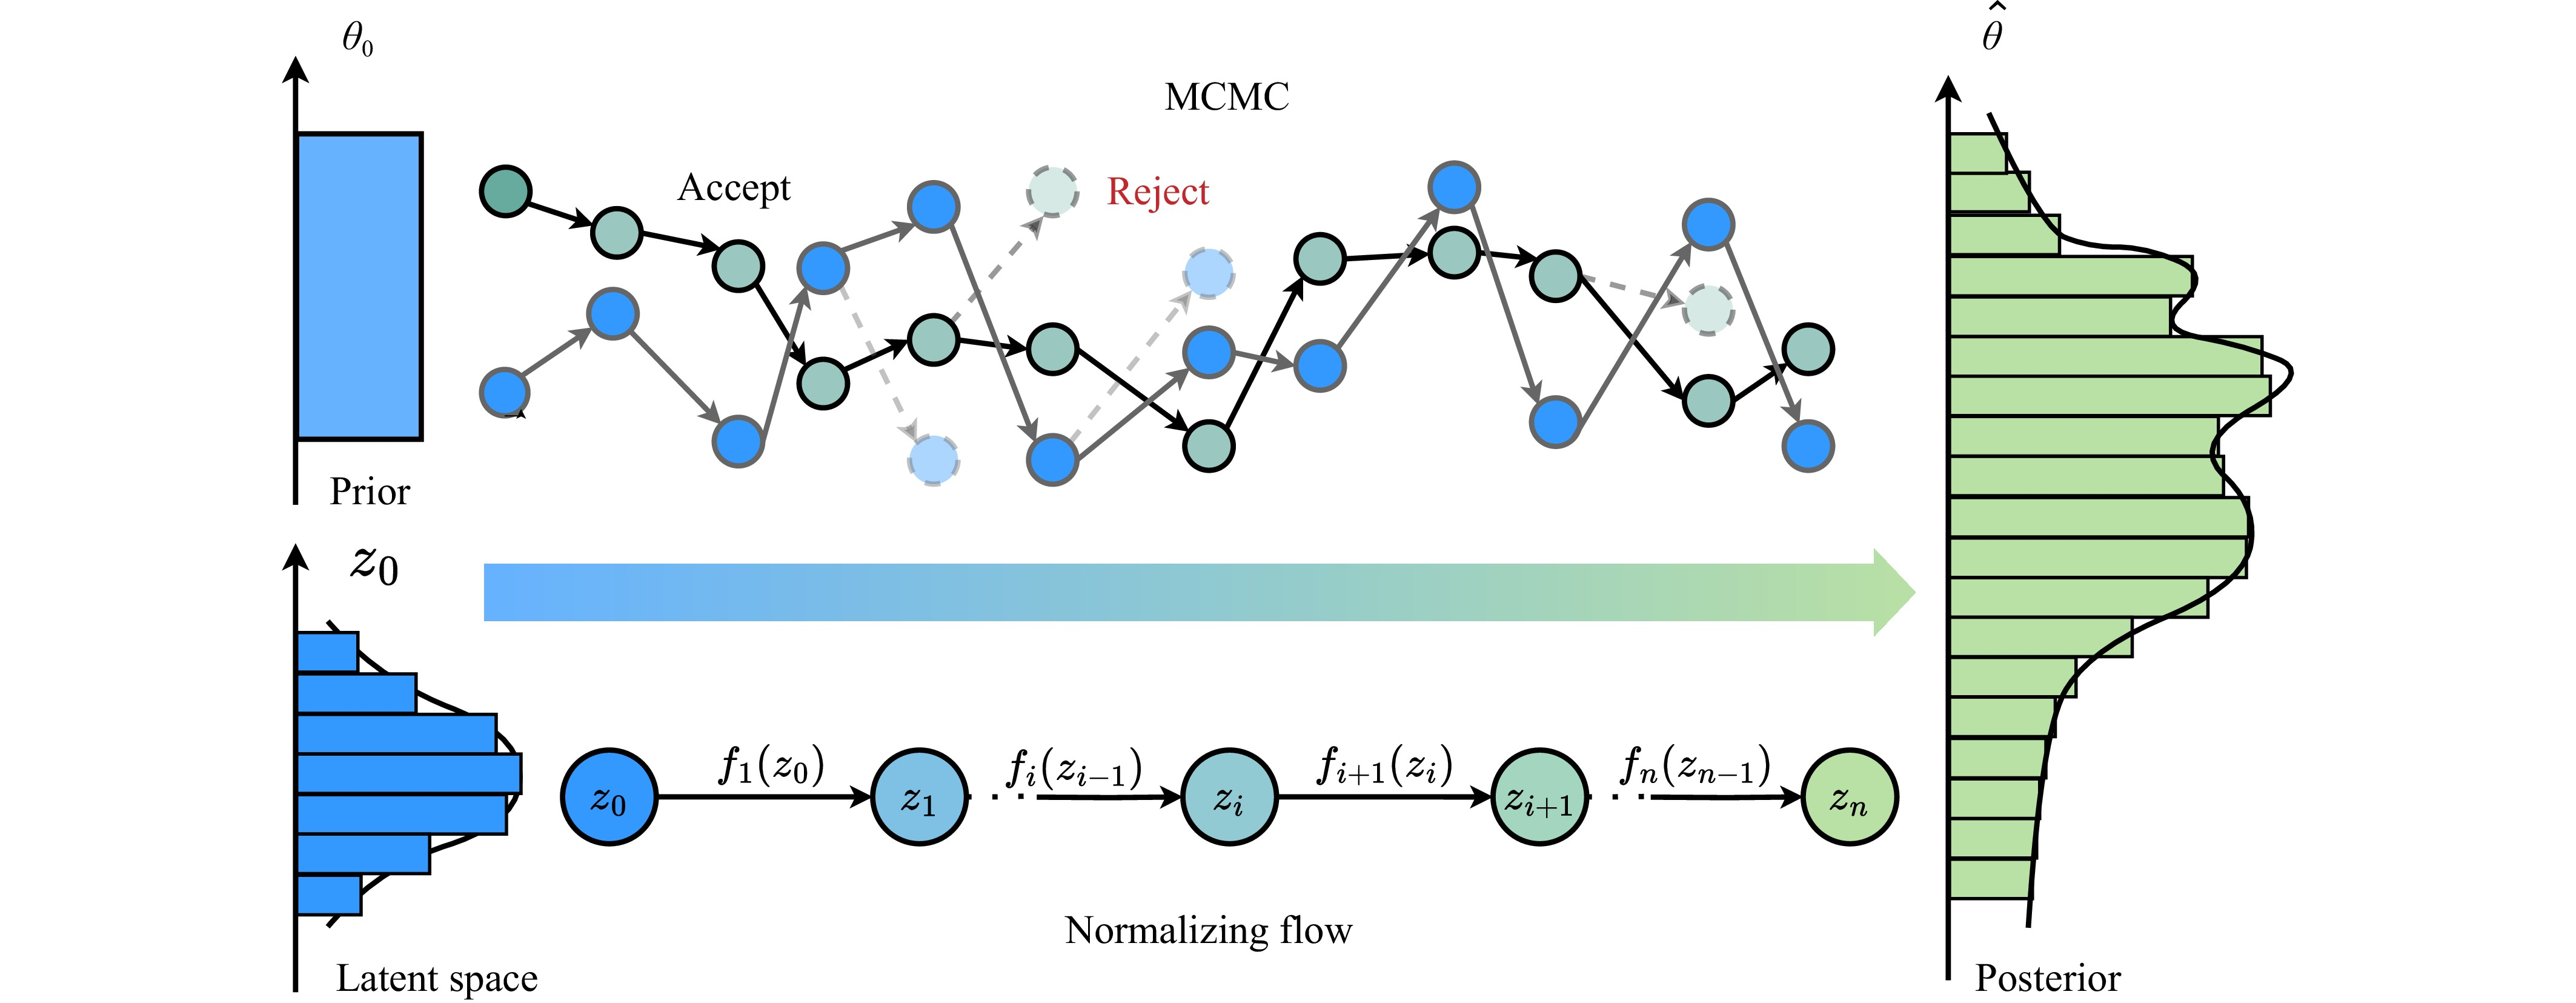
\includegraphics[width=0.96\textwidth]{figures/FOP2025_045301_fig7_mcmc_nf.png}
\caption{传统 MCMC 采样与归一化流后验近似的流程对比。上半部分展示 Metropolis--Hastings 算法从初始参数 $\theta_0$ 出发，经候选采样、接受/拒绝和链式更新逐步收敛到后验样本；下半部分展示归一化流从标准正态潜变量 $z_0$ 出发，通过多层可逆映射生成目标后验样本。该图直观说明了引力波参数估计中从“逐事件迭代采样”向“离线训练、在线快速生成”的方法转变。图引自 Zhao 等~\cite{zhao2025aidawn} 的 Figure 7。}
\label{fig:sbi-vs-mcmc}
\end{figure}

从信息论的视角，SBI 与传统 MCMC 方法代表了两种不同的推断哲学：MCMC 是“计算型推断”（computational inference），通过随机采样逐步积累关于后验分布的信息，每次采样都进行一次完整的信号-噪声匹配计算；SBI 是“学习型推断”（learning-based inference），通过大量离线模拟训练一个“推断引擎”，一旦训练完成就能以较低的计算代价对新数据快速响应。这两种哲学各有其适用场景：当后验分布形状未知且需要最高精度时，MCMC 的完整采样更为可靠；当需要对大量新数据进行快速推断且允许经过校准的近似误差时，SBI 的效率优势非常突出。引力波天文学的未来发展趋势——从少数高优先级事件的精密分析，到海量事件的实时处理——将使 SBI 从“可选的加速工具”逐渐发展为关键的推断基础设施，这正是本章详细介绍 SBI 框架的根本动机。

\section{贝叶斯推断的计算瓶颈与SBI动机}

传统贝叶斯推断方法的计算瓶颈来自两个相互耦合的因素。

\textbf{似然评估代价}。引力波似然函数的标准形式为
\begin{equation}
  \ln p(d|\theta) = -\frac{1}{2}\langle d - h(\theta),\, d - h(\theta)\rangle,
\end{equation}
其中内积 $\langle a, b\rangle = 4\,\mathrm{Re}\int_0^\infty \tilde{a}(f)\tilde{b}^*(f)/S_n(f)\,\mathrm{d}f$ 需要在频域计算，$h(\theta)$ 为给定参数下的理论波形。对于地面探测器的双黑洞系统，单次波形生成约需毫秒量级；但对于空间探测器的 EMRI 系统，精确波形生成可能需要数秒至数分钟，使得 MCMC 的数百万次似然评估在实践中不可行。

为了理解这一瓶颈的严峻程度，可以具体分析一个典型 EMRI 事件的参数估计耗时。精确的 EMRI 波形需要通过求解 Teukolsky 方程（描述小天体在 Kerr 时空中的扰动）来生成，单次求解时间约 1--100 秒，取决于所需频率分辨率和参数配置。若采用嵌套采样方法（Nested Sampling），收敛到充分精确的后验分布通常需要约 $10^6$ 次似然评估；以每次 10 秒计算，总计算时间约为 $10^7$ 秒，折合约 115 天——对于单个事件而言已明显超出常规分析节奏。即便使用现象学近似波形（AK/AAK 模型，每次约 0.1 秒），完整 MCMC 也需要约数天时间，且近似波形的准确性在高质量比、高自旋等极端参数下存疑。

相比之下，地面探测器的双黑洞（BBH）事件参数估计虽然也耗时，但已达到实际可操作的水平。以 GW150914 为例，使用 LALInference（LVK 标准参数估计流水线）在16核 CPU 集群上的运行时间约为 22 小时；更轻量的波形近似（IMRPhenomP）可将时间压缩至约 6 小时。对于大质量 BBH（太极的目标源，啁啾质量 $\mathcal{M} \sim 10^6$--$10^9\,M_\odot$，信号持续数天），时域波形积分时间较长，加上时变响应函数的处理，单次似然评估时间约为 1--10 秒，MCMC 总运行时间可达数月。这一现实使得在太极任务运行期间对每个 MBHB 事件都进行完整 MCMC 参数估计成为奢望，SBI 方法因此不是可选的“加速工具”，而是必要的“基础设施”。

\textbf{引力波后验分布的典型形状}。理解 SBI 方法的设计选择，需要首先理解引力波参数后验分布的典型几何形状。以低质量 BBH 系统（啁啾质量 $\mathcal{M} \sim 15\,M_\odot$）为例，15 维参数空间中各参数的后验分布呈现截然不同的约束精度：

啁啾质量 $\mathcal{M}$ 是约束最紧的参数，后验宽度约为真实值的 0.1\%。这是因为信号的相位演化对 $\mathcal{M}$ 极为敏感（相位约正比于 $\mathcal{M}^{-5/3}$），而当 SNR 较高时，相位测量精度可以达到约 0.1 弧度，对应约 $10^{-3}$ 的质量精度。质量比 $q = m_1/m_2$ 的约束宽度约为真实值的 30\%，是因为当两者质量相差不大时，波形对 $q$ 的敏感性相对较弱（简并于沿等 $\mathcal{M}$ 曲线的方向）。

天空位置（赤经 $\alpha$、赤纬 $\delta$）的约束依赖于探测器的几何配置：双探测器（LIGO H1 和 L1）只能约束信号到达时间差，对应天球上的一个大圆环，后验呈环状；三探测器（H1、L1、Virgo）可以利用两个时间差和振幅比约束，将天区压缩为数十平方度的细长区域。

自旋参数（每个黑洞两个横向自旋分量和一个轴向分量，共六个）的约束通常最弱，后验宽度达到理论范围的 50\%--80\%。高质量比系统中，主星（较重黑洞）的轴向自旋分量（有效自旋 $\chi_{eff}$）约束稍好，而伴星的自旋几乎完全简并。这种极不均匀的约束精度——有的参数约束极紧，有的几乎无约束——使得引力波后验分布在参数空间中呈现出高度非球形的、细长而弯曲的几何形状，传统 MCMC 需要精心设计的提案分布才能高效探索这种形状，SBI 方法则通过归一化流的灵活变换能力直接建模这种复杂几何。

\textbf{参数空间维度}。双黑洞并合系统的参数空间通常为 15 维（两个质量、六个自旋分量、距离、天空位置、轨道倾角、极化角、并合时刻、参考相位），EMRI 系统则多达 17 维，且存在强参数简并（多个参数组合给出相似的波形）。高维简并参数空间中，MCMC 的混合效率极低，需要大量步骤才能充分探索后验分布。

SBI 的核心思想是：在推断阶段之前，利用大量模拟数据（$\theta_i \sim p(\theta)$，$d_i \sim p(d|\theta_i)$）训练神经网络，使其学习参数与数据之间的统计关系~\cite{Cranmer2020SBI}。训练完成后，对新的观测数据 $d_\mathrm{obs}$，网络能够在毫秒至秒级内直接输出后验分布的近似，无需重新运行耗时的采样过程。

引力波似然函数存在一种值得深入分析的特殊代数结构，这一结构既揭示了传统计算方法的瓶颈，也为理解 SBI 方法的加速机理提供了物理基础。在高斯平稳噪声假设下，将内积展开可得：
\begin{equation}
  \ln p(d|\theta) = -\frac{1}{2}\langle d - h(\theta), d - h(\theta)\rangle = \langle d, h(\theta)\rangle - \frac{1}{2}\langle h(\theta), h(\theta)\rangle + \text{const},
\end{equation}
其中常数项 $-\frac{1}{2}\langle d, d\rangle$ 与参数 $\theta$ 无关，不影响参数估计。第一项 $\langle d, h(\theta)\rangle$ 是匹配滤波统计量，可以通过快速傅里叶变换（FFT）高效计算；第二项 $\langle h(\theta), h(\theta)\rangle$ 是模板的自相关函数，仅依赖于波形参数 $\theta$，原则上可以在参数网格上预计算并存储。这一分解说明了匹配滤波的物理本质：扫描模板库等价于在参数空间中搜索使第一项最大（同时第二项适度）的 $\theta$。

然而，这一分解对于精确 MCMC 参数估计的加速潜力是有限的，原因在于：第二项的预计算需要覆盖整个连续参数空间，而参数空间是连续的，不可能在任意精度上预计算所有点；更根本的问题是，每次参数变化都需要重新生成波形 $h(\theta)$，而波形生成本身就是计算瓶颈——对于后牛顿（PN）波形，单次生成约需毫秒级；对于数值相对论拼接波形（如 IMRPhenomXP），单次生成约需数十毫秒；对于精确的 EMRI Teukolsky 波形，单次生成则需秒至分钟级。这种阶梯型的波形生成代价，正是不同引力波源类型的参数估计难度存在量级差异的根本原因。在 SBI 框架中，神经网络在训练阶段学习大量 $(\theta, d)$ 对所包含的统计关系，从而在推断阶段将主要波形生成代价转移到离线训练过程，实现在线推断的显著加速。

归一化流（Normalizing Flows）是 SBI 中最成熟的实现路线~\cite{Papamakarios2021NF,Rezende2015NF}，其核心思想是通过一系列可逆变换将简单的基础分布（如标准正态分布）映射到复杂的目标分布（后验分布）。

\subsection{理论框架}

设 $z \sim p_z(z)$ 为基础分布，$x = f_\phi(z)$ 为可逆变换（参数为 $\phi$），则变换后的分布为
\begin{equation}
  p_\phi(x) = p_z(f_\phi^{-1}(x))\left|\det\frac{\partial f_\phi^{-1}}{\partial x}\right|.
\end{equation}
通过最大化训练数据的对数似然 $\sum_i \ln p_\phi(\theta_i | d_i)$，可以训练网络学习条件后验分布 $p(\theta|d)$。这一框架称为神经后验估计（Neural Posterior Estimation，NPE）~\cite{Dax2021RNPE,Dax2023NPPE}，是引力波参数估计中应用最广泛的 SBI 变体。Green 和 Gair~\cite{Green2021CVAE} 率先将 NPE 应用于 GW150914 的完整参数推断，展示了神经网络可以在单次前向传播（约1秒）内给出与 LALInference 完整贝叶斯分析高度一致的后验分布，证明了 NPE 在真实引力波事件上的可行性。

除 NPE 外，SBI 还包含神经似然估计（NLE，学习似然函数 $p(d|\theta)$）和神经比率估计（NRE，学习似然比 $p(d|\theta)/p(d)$）等变体。Liang 和 Wang~\cite{liang2026sbireview} 的综述系统梳理了这些方法的理论联系与适用场景：NPE 在推断速度上最快（单次前向传播即可），NLE 和 NRE 则在某些情形下对先验变化更鲁棒。

\textbf{NPE、NLE、NRE 的比较}。三类 SBI 方法各有其适用场景，理解它们之间的差异对于选择合适的方法至关重要。NPE（神经后验估计）直接训练网络学习条件后验分布 $q_\phi(\theta|d) \approx p(\theta|d)$，推断时只需将观测数据 $d_{obs}$ 通过网络进行一次前向传播，即可获得后验样本，推断时间为 $O(1)$。NPE 的主要缺点是对先验分布的变化不鲁棒：训练时使用先验 $p(\theta)$，若推断时先验改变（如加入额外的天体物理约束），模型需要重新训练或使用重要性采样修正，后者计算代价较高。

NLE（神经似然估计）训练网络学习似然函数 $q_\phi(d|\theta) \approx p(d|\theta)$，在推断时将学习到的似然函数代入贝叶斯定理，结合 MCMC 或嵌套采样进行完整的贝叶斯推断。NLE 的优点是：由于它学习的是与先验无关的似然函数，先验的修改不需要重新训练网络，只需重新运行（现在廉价的）MCMC 即可——因为 MCMC 的计算瓶颈本是似然评估，而现在似然评估已被神经网络替代，大幅加速。NLE 的缺点是推断仍需要 MCMC，比 NPE 慢若干量级。

NRE（神经比率估计）训练网络学习似然比 $r_\phi(d, \theta) \approx p(d|\theta)/p(d)$，通过对比正样本（$(\theta, d) \sim p(\theta)p(d|\theta)$）和负样本（$(\theta, d) \sim p(\theta)p(d)$）来训练分类器，并将训练好的分类器输出转化为似然比。NRE 对先验变化通常具有较强鲁棒性，且训练较稳定（二分类损失函数性质良好），但推断速度介于 NPE 和 NLE 之间（需要 MCMC 但评估代价极低）。在引力波参数估计的实践中，当先验需要频繁修改（如结合电磁观测引入的天空位置约束）时，NRE 或 NLE 是更合理的选择；当需要快速处理大量事件且先验固定时，NPE 的推断速度优势更为突出。Lueckmann 等人~\cite{Lueckmann2021benchmarking}对 NPE、NLE、NRE 三类方法在多个基准任务上进行了系统性对比，发现三者的相对优势高度依赖于任务结构，为方法选择提供了重要的实证依据。

\subsection{归一化流的常见架构}

实现归一化流的关键是设计既可逆又具有高效雅可比行列式计算的变换。常见架构包括：

\textbf{仿射耦合层}（Affine Coupling Layers）：将输入向量分为两部分，一部分通过神经网络参数化另一部分的仿射变换。这一设计使得正向和逆向变换都高效可计算，雅可比行列式为对角矩阵，计算代价为 $O(d)$。Real NVP（Real-valued Non-Volume Preserving）是最具代表性的仿射耦合架构：将 $d$ 维输入分为两半 $(x_1, x_2)$，变换规则为 $y_1 = x_1$，$y_2 = x_2 \odot \exp(s(x_1)) + t(x_1)$，其中 $s(\cdot)$ 和 $t(\cdot)$ 为任意神经网络（分别给出缩放因子和平移量），$\odot$ 为逐元素乘法。该变换的雅可比行列式为 $\prod_i \exp(s_i(x_1))$，计算量仅为 $O(d)$；逆变换为 $x_1 = y_1$，$x_2 = (y_2 - t(y_1))/\exp(s(y_1))$，同样简单高效。通过交替分组方式（每层交换哪半部分被变换）堆叠多个仿射耦合层，可以建模任意复杂的分布。

\textbf{自回归流}（Autoregressive Flows）：MAF（Masked Autoregressive Flow）利用 MADE（掩码自编码器）实现自回归结构：变换规则为 $y_i = x_i \cdot \exp(\alpha_i(x_{<i})) + \mu_i(x_{<i})$，其中 $\alpha_i$ 和 $\mu_i$ 仅依赖于第 $i$ 维之前的所有维度。训练时前向计算（给定 $x$ 计算 $y$）只需 $O(d)$ 时间（所有维度可并行计算），但采样（给定 $y$ 恢复 $x$）需要顺序计算，每一维的恢复依赖于前面维度的结果，计算量为 $O(d^2)$，使得采样速度较慢。IAF（Inverse Autoregressive Flow）与 MAF 互为逆变换：采样速度快（$O(d)$），但训练时的密度估计需要顺序计算。在引力波参数估计中，推断阶段需要频繁采样（对每个新事件都需要生成大量后验样本），因此 IAF 的快速采样特性更受青睐；但 MAF 在训练阶段更为高效，实践中往往先训练 MAF 再转化为等价的 IAF 格式。

\textbf{神经样条流}（Neural Spline Flows，NSF）：用单调有理二次样条（monotone rational-quadratic splines）替代仿射变换。每个维度的变换由 $K$ 个控制点（control points）参数化，这些控制点的位置和切线方向都是可学习的，因此 NSF 的表达能力强于仿射变换（仿射变换只有两个自由参数：缩放和平移）。样条变换保持严格单调性（从而保证可逆性），且其雅可比行列式可以解析计算（$O(d)$）。在引力波参数估计的实践中，NSF 是表现较好的离散流架构之一：对于 15 维的 BBH 参数空间，使用 $K = 8$ 个控制点的 NSF 通常能在合理训练时间（约 12 小时，单 GPU）内达到与 MCMC 相近的精度，而仿射耦合层往往需要更多层数或更宽的网络才能实现类似表达能力。

\textbf{条件归一化流的训练}。在 SBI 框架下，流的目标是近似条件后验分布 $p(\theta|d)$ 而非无条件分布 $p(\theta)$。实现条件化的标准方式是：在网络的每一层，将观测数据 $d$ 通过一个编码器网络（通常是 CNN 或 Transformer）映射为嵌入向量 $c = f_{enc}(d)$，然后以 $c$ 为额外输入（条件输入）加入流的每一层变换（仿射变换中的 $s$ 和 $t$ 函数以 $c$ 为额外输入，从而让每一层的变换依赖于具体的观测数据）。训练目标为：
\begin{equation}
  \min_\phi \mathbb{E}_{(\theta, d) \sim p(\theta)p(d|\theta)} [-\log q_\phi(\theta|d)],
\end{equation}
即最小化神经网络估计的后验与真实后验之间的 KL 散度（由于期望是关于联合分布 $p(\theta, d)$ 的，可以通过模拟样本对期望进行无偏估计）。训练完成后，对新的观测 $d_{obs}$，首先计算嵌入向量 $c = f_{enc}(d_{obs})$，然后从基础分布 $p_z(z)$ 采样潜变量 $z$，通过流的前向变换 $\theta = f_\phi(z; c)$ 得到后验样本，整个过程只需毫秒量级的前向传播，无需任何迭代优化。

\subsection{先验知识引导的归一化流训练}

高维参数空间中，均匀采样的训练数据在参数空间中分布稀疏，模型难以学习物理上重要但参数空间中稀少的区域（如高质量比、高自旋等极端情形）的特征。Wang 等人~\cite{wang2022normflow} 提出从物理上期望的中间分布采样来构建训练数据集，使高维特征空间中物理上更重要的区域获得更密集的数据覆盖。

这一先验知识采样策略将物理先验转化为训练数据的分布设计。训练完成后，模型在单块 V100 GPU 上约 1 秒内生成数千个后验样本，验证了在高维引力波数据推断中的有效性。

SBI与主动学习的结合，进一步突破了标准训练集覆盖范围对推断性能的限制。当训练数据有限时，均匀先验采样往往将大量模拟配额浪费在后验概率极低的参数区域，导致神经网络对高后验区域的刻画精度不足。主动学习（active learning）提供了一种根本性的解决思路：不从均匀先验中采样训练数据，而是根据当前模型对参数空间的不确定性估计，将后续模拟集中在最有价值的区域。顺序神经后验估计（SNPE，Sequential Neural Posterior Estimation）是这一思路的代表性实现：在每轮“模拟—训练”循环中，算法基于当前近似后验的估计结果，将下一轮模拟集中在高后验区域，逐步收缩有效搜索空间。对于引力波参数估计，SNPE可以将达到同等精度所需的模拟次数减少约50\%至80\%，对于计算代价高昂的EMRI波形生成而言尤为重要——若仅需减少50\%的训练波形，总训练时间可从数天压缩至数小时，使原本不可行的在轨实时重训练成为可能。这一主动学习范式代表了SBI方法由“一次性离线训练”向“迭代自适应训练”演进的重要方向，也是应对未来海量引力波事件时代计算资源分配挑战的关键策略之一。

\subsection{太极任务的归一化流参数估计}

Du、Liang、Wang 等人~\cite{du2024normflow} 将归一化流方法应用于太极任务的大质量双黑洞系统参数估计，面对三项特有挑战：混淆噪声（大量波源信号叠加）、时变响应函数（太极星座一年周期的轨道运动导致探测器响应随时间变化）、以及到达时间参数的额外多模态结构。

\textbf{时变响应函数的处理}。太极由三颗卫星组成三角星座，绕日公转（轨道半径约 1 AU），轨道周期为一年。星座相对于遥远引力波源的指向因此随时间变化，导致探测器的方向响应函数（天线方向图）呈周期性变化。对于持续数小时至数天的 MBHB 信号，若采用固定响应函数的近似（忽略指向变化），会引入系统性波形误差，进而导致参数估计偏差。对于持续时间较短（数小时内）的并合阶段，可以采用“分段常数”近似：将信号持续时间分为若干段，每段内使用固定的响应函数，段长通常取为 $\sim$30 分钟（此时指向变化引起的响应误差小于 1\%）。但对于旋进阶段持续数天至数周的长时信号，分段近似需要分为数百段，使波形生成复杂度倍增。Du 等采用“变换映射”（transformed parameterization）策略：将时变响应函数的效应通过参数重定义吸收入信号参数中，允许归一化流直接学习时变响应的统计效应，而无需在训练数据生成阶段显式模拟每个时间段的响应变化。

\textbf{后验分布的多模态结构}。太极对 MBHB 事件的天空位置后验分布，由于时变响应函数的存在，会呈现出比地面探测器更复杂的多模态结构。在不同时刻的响应函数组合下，存在 4--8 个不同的（天空位置，极化角）组合给出几乎等价的观测信号，从而形成多个似然极大值。相比之下，地面双探测器配置（H1 + L1）的天空位置后验通常形成一个大圆环（对应固定时间延迟），而 Virgo 的加入将圆环压缩为两个区域，多模态结构相对简单。太极的 4--8 个极大值要求归一化流具有足够强的多模态建模能力。研究发现，通过采用分层变换的组合（先建模单模态的基础分布，再通过混合变换引入多模态），归一化流能够准确重现这种复杂的多模态结构，而标准的单峰高斯变分推断则完全无法捕获这一特性。

\section{归一化流的理论框架与结构选择}

图~\ref{fig:sbi-vs-mcmc} 强调的是 MCMC 与归一化流之间的计算范式差异；进一步看，SBI 并不等同于单一的归一化流模型，而是一组围绕“模拟器可用、解析似然困难”的推断策略。图~\ref{fig:sbi_variants} 总结了五类代表性路线：神经后验估计（NPE）直接学习 $p(\theta|d)$，推断速度最快；神经比率估计（NRE）与神经似然估计（NLE）分别学习似然比和似然函数，通常仍需与 MCMC 结合，但在先验替换和后验校正上更灵活；流匹配后验估计（FMPE）通过神经网络学习从基分布到后验分布的连续流；一致性模型后验估计（CMPE）则试图用更少采样步数逼近概率流。它们共同体现了 SBI 的核心思想：把逐事件的昂贵采样，转化为可并行、可复用、但必须经过校准验证的学习问题~\cite{liang2026sbireview}。

\begin{figure}[htbp]
\centering
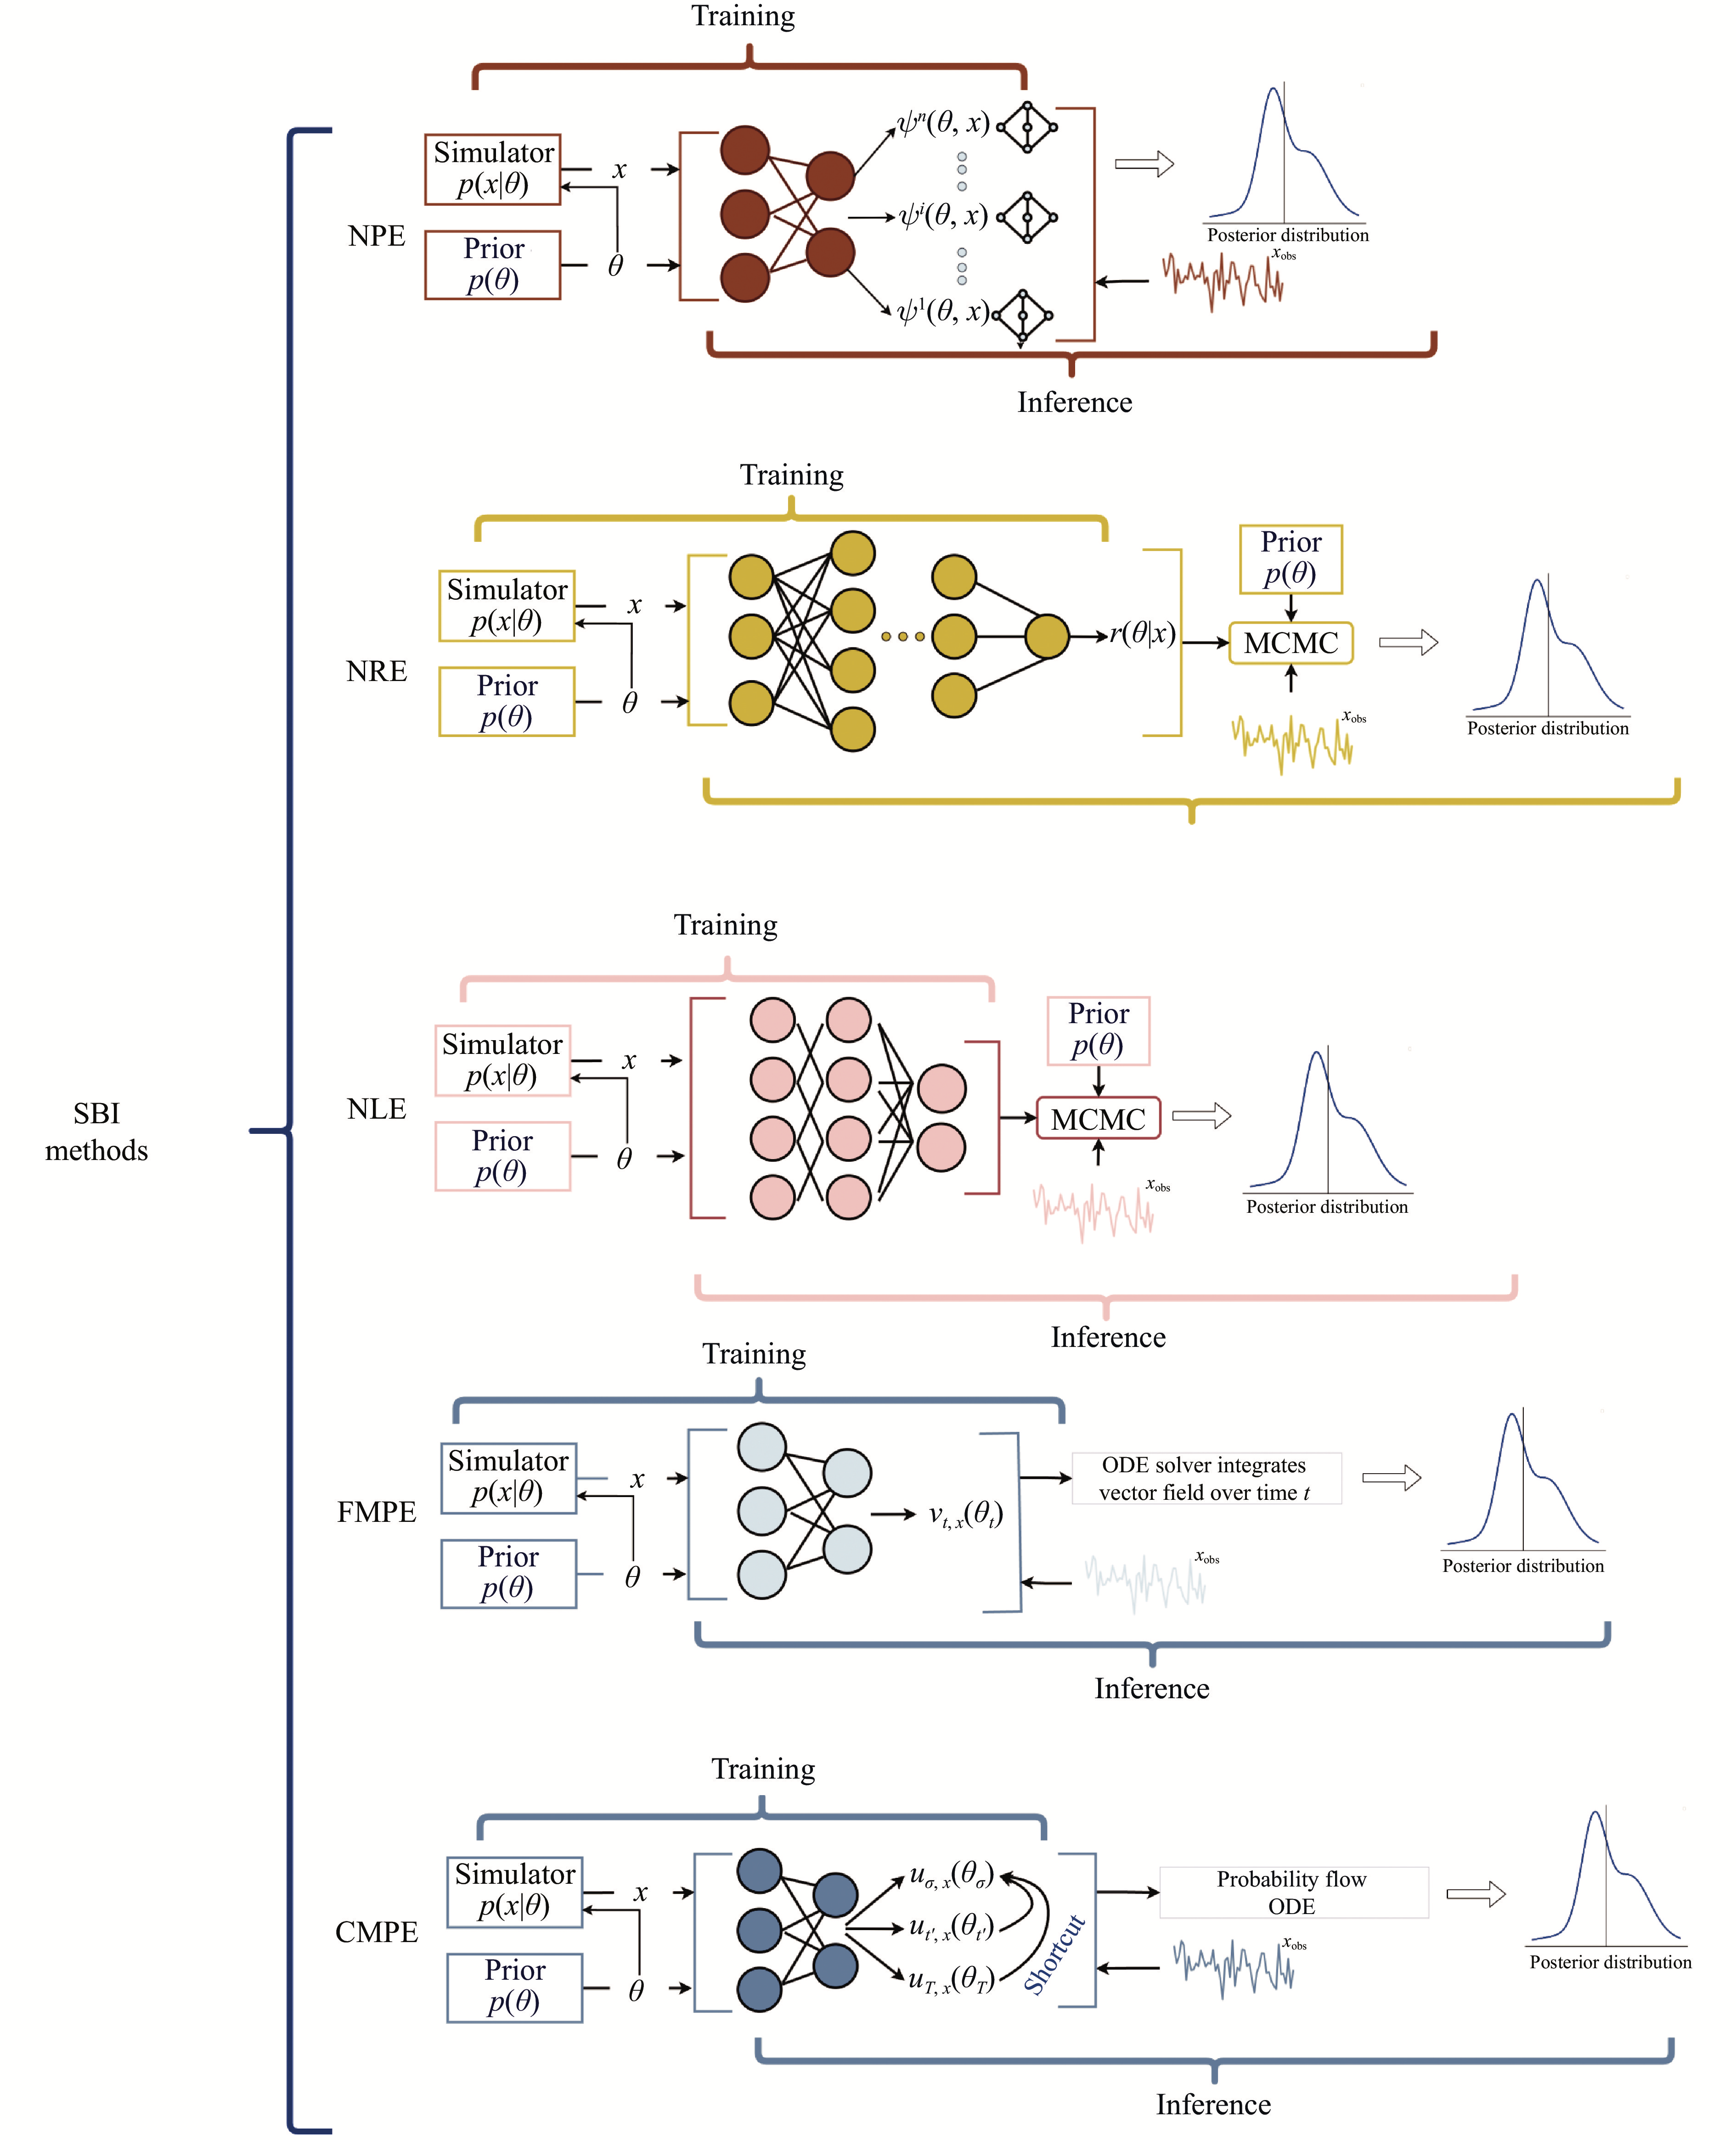
\includegraphics[height=0.76\textheight,keepaspectratio]{figures/ATI2026_sbi_review_fig1.png}
\caption{五类主要 SBI 方法的训练与推断流程概览。NPE 直接近似条件后验；NRE 和 NLE 分别估计似然比与似然函数，并通常与 MCMC 结合获得后验样本；FMPE 通过 ODE 概率流刻画后验；CMPE 用一致性模型学习概率流以提高采样效率。这些方法共同构成了引力波快速贝叶斯参数估计的主要技术谱系。图引自 Liang 和 Wang~\cite{liang2026sbireview} 的 Figure 1。}
\label{fig:sbi_variants}
\end{figure}

归一化流（Normalizing Flows）是当前 SBI 框架中最主流的后验近似工具。其核心思想是通过一系列可逆变换，将一个简单的基础分布（通常为标准正态分布）逐步“变形”为复杂的目标分布。本节从概率密度变换的基本公式出发，系统梳理仿射耦合层、神经样条流等主流架构的设计原理，并讨论条件化策略在引力波数据分析中的具体实现。

\subsection{变量变换公式与雅可比行列式}

设 $Z \sim p_Z(z)$ 为基础分布（如标准正态分布），$f: \mathbb{R}^d \to \mathbb{R}^d$ 为可逆变换，令 $X = f(Z)$，则 $X$ 的概率密度由变量变换公式给出：
\begin{equation}
  p_X(x) = p_Z\!\left(f^{-1}(x)\right) \left|\det J_{f^{-1}}(x)\right|,
\end{equation}
其中 $J_{f^{-1}}(x) = \partial f^{-1}(x)/\partial x$ 为逆变换的雅可比矩阵，$|\det J_{f^{-1}}|$ 为其行列式的绝对值，反映了变换在 $x$ 处的局部体积缩放比例~\cite{Papamakarios2021NF}。等价地，若以正向变换 $f$ 表达，则：
\begin{equation}
  \ln p_X(x) = \ln p_Z(z) - \ln\left|\det J_f(z)\right|, \quad z = f^{-1}(x).
\end{equation}
归一化流通过堆叠 $L$ 个可逆变换 $f = f_L \circ f_{L-1} \circ \cdots \circ f_1$，将对数似然分解为各层雅可比行列式之和：
\begin{equation}
  \ln p_X(x) = \ln p_Z(z_0) - \sum_{l=1}^{L} \ln\left|\det J_{f_l}(z_{l-1})\right|,
\end{equation}
其中 $z_0 = f^{-1}(x)$ 为基础分布中的对应点，$z_l = f_l(z_{l-1})$ 为各层输出。

可逆性是归一化流的必要条件：若变换不可逆，则无法从基础分布采样并映射到目标分布，也无法计算精确的概率密度。然而，可逆性本身并不足以保证计算可行性——对于一般的 $d \times d$ 矩阵，行列式的计算复杂度为 $O(d^3)$（LU 分解），当 $d$ 达到数十维时（如 BBH 的 15 维参数空间），每次前向传播都需要计算高维矩阵行列式，训练过程中数百万次的梯度更新会使总计算量迅速增大到难以接受的程度。

归一化流的核心设计思想正是通过对变换结构施加特殊约束，将雅可比行列式的计算从 $O(d^3)$ 降至 $O(d)$。具体而言，若雅可比矩阵为三角矩阵（上三角或下三角），则其行列式等于对角元素之积，计算量仅为 $O(d)$；若雅可比矩阵为对角矩阵，则计算更为简单。仿射耦合层和自回归流均通过不同方式实现了三角或对角雅可比结构，从而在保持强表达能力的同时，将密度估计的计算代价控制在线性量级。

\subsection{仿射耦合层与 Real NVP}

仿射耦合层（Affine Coupling Layer）是归一化流中最具代表性的基础构件，由 Dinh 等人在 Real NVP（Real-valued Non-Volume Preserving）框架中系统提出~\cite{Dinh2017RealNVP}。其核心思想是将 $d$ 维输入向量分为两组：前 $k$ 维 $x_1 \in \mathbb{R}^k$ 保持不变，后 $d-k$ 维 $x_2 \in \mathbb{R}^{d-k}$ 通过依赖于 $x_1$ 的仿射变换进行映射：
\begin{equation}
  y_1 = x_1, \qquad y_2 = x_2 \odot \exp\!\left(s(x_1)\right) + t(x_1),
\end{equation}
其中 $s(\cdot): \mathbb{R}^k \to \mathbb{R}^{d-k}$ 和 $t(\cdot): \mathbb{R}^k \to \mathbb{R}^{d-k}$ 为任意神经网络（分别给出逐元素的对数缩放因子和平移量），$\odot$ 为逐元素乘法。

该变换的雅可比矩阵具有下三角块结构：
\begin{equation}
  J_f = \begin{pmatrix} I_k & 0 \\ \partial y_2/\partial x_1 & \mathrm{diag}(\exp(s(x_1))) \end{pmatrix},
\end{equation}
其行列式为 $\det J_f = \prod_{i=1}^{d-k} \exp(s_i(x_1))$，计算量仅为 $O(d)$，与参数空间维度成线性关系。逆变换同样高效：$x_1 = y_1$，$x_2 = (y_2 - t(y_1)) \odot \exp(-s(y_1))$，无需任何迭代求解。

单个仿射耦合层的表达能力受限，因为 $x_1$ 部分在每层中保持不变。Real NVP 通过交替分组策略（Alternating Partitioning）解决这一问题：奇数层变换后 $d-k$ 维，偶数层变换前 $k$ 维，使得每个维度在若干层后都经历了变换。在引力波参数估计的实践中，通常堆叠 8 至 16 个仿射耦合层，每层的 $s(\cdot)$ 和 $t(\cdot)$ 网络采用 4--6 层全连接网络（宽度 128--512），总参数量约为 $10^6$--$10^7$。这一规模在单块 GPU 上可在 12--24 小时内完成训练，推断时单次前向传播仅需约 1 毫秒，满足引力波事件实时处理的需求。

\subsection{神经样条流（NSF）的表达能力优势}

仿射耦合层的根本局限在于其变换的线性性：对于固定的 $x_1$，$y_2$ 关于 $x_2$ 的变换是仿射的（线性加偏置），每个维度只有两个自由参数（缩放和平移）。这意味着单层仿射耦合层只能建模单峰、近似高斯的条件分布，对于多模态或高度非高斯的后验分布，需要堆叠大量层数才能达到足够的表达能力。

神经样条流（Neural Spline Flows，NSF）通过用单调有理二次样条（Monotone Rational-Quadratic Splines）替代仿射变换，从根本上提升了单层的表达能力~\cite{Durkan2019NSF}。具体而言，对于每个维度 $i$，NSF 将变换区间 $[a, b]$ 划分为 $K$ 个子区间，由 $K+1$ 个控制点 $\{(x_k^{(i)}, y_k^{(i)})\}_{k=0}^{K}$ 和对应的切线方向 $\{d_k^{(i)}\}_{k=0}^{K}$ 参数化。在每个子区间内，变换由有理二次函数给出，保证严格单调性（从而保证可逆性）。整个样条变换由 $3K - 1$ 个可学习参数（$K-1$ 个内部节点位置、$K$ 个高度差、$K+1$ 个切线方向）完全确定，其雅可比行列式可以解析计算，计算量为 $O(d)$。

与仿射变换相比，NSF 的表达能力优势显著。对于 15 维 BBH 参数空间（质量、自旋、天空位置、距离、倾角等），使用 $K = 8$ 个控制点的 NSF 通常能以约 30\% 更少的层数达到与仿射耦合层相同的后验近似精度：仿射耦合层通常需要 12--16 层，而 NSF 仅需 8--12 层即可实现等价的 Jensen-Shannon 散度（相对于 MCMC 参考后验）。这一差异在高度非高斯的参数（如天空位置的赤经赤纬、轨道倾角）上尤为突出，因为这些参数的后验分布往往呈现出明显的非对称性或多峰结构，仿射变换难以在单层内捕获。

计算代价方面，样条变换比仿射变换慢约 2--3 倍（主要来自样条系数的查找和有理函数求值），但由于所需层数减少，总体训练时间通常相当甚至更短。在推断阶段，NSF 的单次前向传播时间约为 2--5 毫秒（15 维，10 层，批量大小 1000），仍远快于任何基于 MCMC 的方法。综合考虑精度与效率，NSF 是当前引力波参数估计中离散归一化流的首选架构。

\subsection{条件化策略：数据编码器的设计}

在 SBI 框架下，归一化流的目标是近似条件后验分布 $p(\theta|d)$ 而非无条件分布 $p(\theta)$。实现条件化的标准方式是引入数据编码器：将观测数据 $d$（时域或频域引力波应变）通过编码器网络 $f_{enc}$ 映射为固定维度的嵌入向量 $c = f_{enc}(d) \in \mathbb{R}^{d_c}$，然后以 $c$ 为条件输入加入流的每一层变换——仿射变换中的 $s(\cdot)$ 和 $t(\cdot)$ 函数以 $c$ 为额外输入，从而使每层的变换依赖于具体的观测数据。

编码器架构的选择对整体性能有重要影响，需根据数据的时频特性和计算约束综合考量：

\textbf{一维卷积神经网络（1D CNN）}适用于处理时域引力波数据。典型架构包含 4--8 个卷积层（核大小 8--32，步长 2--4），通过逐步下采样将长度为 $\sim 10^4$--$10^5$ 的时域序列压缩为 64--256 维的嵌入向量。1D CNN 的优势在于计算效率高（单次前向传播约 0.1--0.5 毫秒）、对局部时域特征（如并合时刻的波形形态）敏感，且通过卷积的平移等变性对信号到达时间具有一定的鲁棒性。其局限是感受野有限，对长时旋进阶段的全局相位演化捕获能力较弱。

\textbf{Transformer 编码器}适用于处理长时序列（如 EMRI 信号的数年旋进过程）。自注意力机制使 Transformer 能够直接建模序列中任意两个时刻之间的依赖关系，感受野覆盖整个序列长度。代价是计算复杂度为 $O(T^2)$（$T$ 为序列长度），对于 $T \sim 10^5$ 的长序列，需要采用线性注意力或分块注意力等近似方法将复杂度降至 $O(T)$。

\textbf{频域 CNN}适用于处理白化后的频域数据（功率谱密度归一化后的复数频域应变）。由于引力波探测器的噪声功率谱密度在频域中变化平缓，白化后的频域数据具有近似平稳的统计特性，适合用标准 2D CNN（将实部和虚部视为两个通道）处理。频域 CNN 在计算效率和对噪声特性的适应性上具有优势，是 LIGO/Virgo 数据分析中最常用的编码器选择。

嵌入维度 $d_c$ 的选择需要在信息压缩率和表达能力之间权衡。过小的 $d_c$（如 32 维）可能导致信息瓶颈，使编码器无法保留足够的参数估计信息；过大的 $d_c$（如 512 维）则增加流网络的参数量和训练难度。实践中，$d_c = 64$--$256$ 维是常见选择，具体取值通常通过在验证集上监测后验近似质量（如与 MCMC 参考后验的 Jensen-Shannon 散度）来确定。

编码器与流的训练策略有两种主要方式：联合训练（Joint Training）将编码器和流的参数同时优化，以端到端的方式最大化训练数据的对数似然；分阶段训练（Two-Stage Training）先单独预训练编码器（如通过对比学习或重建损失），再固定编码器参数训练流。联合训练通常能达到更好的最终性能，因为编码器可以学习到对参数估计最有用的数据表示，而非通用的数据重建特征；但联合训练对学习率调度和批量大小更为敏感，训练稳定性略差。

在太极 MBHB 任务中，时变响应函数带来了额外的编码挑战：探测器对引力波的响应随轨道相位变化，使得同一参数组合在不同观测时段产生不同的数据特征。Du 等人~\cite{du2024normflow} 的工作表明，通过联合训练策略，编码器能够隐式学习时变响应函数的统计规律，将其效应吸收入嵌入向量 $c$ 中，无需在流的架构中显式建模时变性。这一结果说明，足够容量的编码器（嵌入维度 128 维，6 层 1D CNN）配合端到端训练，可以自动发现并利用数据中与参数估计相关的时变特征，为处理未来空间引力波探测任务中更复杂的时变效应提供了重要参考。

\section{连续归一化流与流匹配：下一代 SBI 方法}

离散归一化流通过有限个可逆变换层构建，其表达能力受限于变换层数和结构。连续归一化流（Continuous Normalizing Flows，CNF）将变换过程连续化，通过常微分方程（ODE）描述从基础分布到目标分布的连续演化：
\begin{equation}
  \frac{\mathrm{d}z(t)}{\mathrm{d}t} = v_\phi(z(t), t),
\end{equation}
其中 $v_\phi$ 为神经网络参数化的速度场。流匹配（Flow Matching）技术~\cite{Lipman2022FlowMatching}通过直接回归目标速度场来训练 CNF，避免了传统 CNF 训练中的数值 ODE 求解，大幅提升训练效率。

\subsection{CNF 用于大质量双黑洞参数估计}

Liang 等人~\cite{liang2024cnfmbhb} 将基于流匹配的 CNF 应用于太极任务的大质量双黑洞参数估计。相比早期的离散归一化流工作，CNF 在表达能力和训练稳定性上有所改进，实现了比传统 MCMC 方法快几个数量级的统计一致参数估计，为太极任务实时数据处理提供了更高效的工具。

\subsection{CNF 应用于 EMRI 参数估计}

极端质量比旋入（EMRI）的参数估计是引力波数据分析中最困难的问题之一：17 维参数空间、强参数简并（多极大值似然函数）、以及极高的计算时间复杂度，使传统 MCMC 方法在实践中面临严峻的计算压力。

\textbf{EMRI 后验的特殊挑战}。EMRI 系统由一个质量约 $10$--$10^2\,M_\odot$ 的致密天体（小天体）绕质量约 $10^5$--$10^7\,M_\odot$ 的大质量黑洞（中心天体）旋转组成，质量比 $q = m_{small}/m_{large} \sim 10^{-5}$--$10^{-3}$。信号特征是长达数年的极复杂旋进过程：小天体在大质量黑洞的弯曲时空中沿近似 Kerr 测地线运动，轨道包含三个基本频率（径向频率 $\Omega_r$、极角频率 $\Omega_\theta$、方位角频率 $\Omega_\phi$），形成高度复杂的李萨如图案。信号的总相位在整个观测周期内可积累约 $10^5$ 弧度，相比之下双黑洞并合信号约 $10^3$ 弧度，这使得 EMRI 参数估计对波形精度的要求极为苛刻（一个相位误差超过约 $0.1$ 弧度就会导致匹配滤波 SNR 的显著下降）。

在参数空间的几何结构上，EMRI 似然函数呈现“阶梯”（ladder）结构：每半个径向轨道周期（约数小时至数天），似然函数出现一个局部极大值，总极大值数可达 $10^4$。这种“阶梯地形”对 MCMC 采样造成严重困难：传统 MCMC 的随机游走提案会被局部极大值“捕获”，在单个极大值附近反复采样，而难以在可接受的计算时间内遍历主要极大值区域。即便使用并行回火（Parallel Tempering）等高级 MCMC 技术，对单个 EMRI 事件的完整后验采样也可能需要约 $10^6$ 核时。CNF 通过流匹配直接学习从先验到后验的概率变换，不需要在后验地形上进行逐步随机游走，理论上可以缓解 MCMC 的“阶梯地形收敛困难”。

Liang 等人~\cite{liang2024cnfemri} 将机器学习方法（具体为基于流匹配的 CNF）系统应用于 EMRI 信号的贝叶斯后验参数估计。训练数据包含 5000 条 EMRI 模拟数据（使用 AAK 近似波形，每条约 0.1 秒生成），参数从先验分布中采样（覆盖质量比、轨道偏心率、轨道倾角、初始频率等全部 17 个参数）。在 GPU（单张 V100）上训练约 24 小时后，对 100 个独立测试事件的评估表明：CNF 估计的后验与真实参数的覆盖率（coverage）接近理论值——P-P 图（probability-probability plot）接近对角线，说明 CNF 的后验估计在该模拟设置下具有统计自洽性。推断时间约 0.1--1 秒每个事件，相比逐事件MCMC可实现多个量级的加速，是机器学习方法进入 EMRI 参数估计这一困难问题的重要系统性尝试。

流匹配与最优传输方法的理论基础值得单独阐述，因为它代表了 CNF 训练范式的根本性改进。传统 CNF 的训练依赖于对概率流 ODE 的数值积分：为了评估给定参数点的对数似然，需要从 $t=0$（基础分布）到 $t=1$（目标分布）数值积分 ODE，计算路径上的雅可比迹（即 $\int_0^1 \mathrm{tr}(\partial v_\phi/\partial z)\,dt$），这需要对 ODE 进行约100步的数值积分，且每步都需要一次神经网络前向传播，训练代价极高。流匹配（Flow Matching）绕过了这一困难：它直接监督速度场 $v_\phi(z, t)$ 拟合目标速度场 $u_t(z|z_1)$，将训练目标转化为普通的回归问题：
\begin{equation}
  \mathcal{L}_{FM} = \mathbb{E}_{t, z_0 \sim p_0, z_1 \sim p_1} \left[ \|v_\phi(z_t, t) - (z_1 - z_0)\|^2 \right],
\end{equation}
其中 $z_t = (1-t)z_0 + tz_1$ 是基础分布样本 $z_0$ 和目标分布样本 $z_1$ 之间的线性插值路径（条件流），$(z_1 - z_0)$ 是沿线性插值路径的恒定速度。由于训练目标仅需要单次前向传播（计算 $v_\phi$ 并与目标速度对比），不需要 ODE 积分，训练效率大幅提升。

最优传输（Optimal Transport，OT）流匹配进一步优化了插值路径的选择。在标准流匹配中，基础样本 $z_0$ 和目标样本 $z_1$ 是独立匹配的（从各自分布中独立采样），插值路径可能出现“交叉”现象——不同插值路径在 $t \in (0,1)$ 区间内相互穿越，导致速度场 $v_\phi$ 在交叉区域需要同时拟合多个相反的速度方向，增大了学习难度。OT 流匹配通过选择最优传输映射（使总运输代价 $\sum_i \|z_{0,i} - z_{1,\sigma(i)}\|^2$ 最小化的排列 $\sigma$）来匹配 $z_0$ 和 $z_1$，从而使插值路径尽可能不交叉，速度场更平滑，网络更容易拟合。在太极 MBHB 和 EMRI 任务上，基于 OT 流匹配的 CNF 比早期离散归一化流方法训练速度快约5倍，在相同训练时间下后验精度提升约10--15\%。这一进步为在更大规模的参数空间（如 EMRI 的17维或包含多源的全局拟合场景）上应用 CNF 奠定了计算效率基础。

CNF在空间引力波全局拟合框架中的角色值得单独讨论，因为全局拟合是太极/LISA数据分析最核心、也最具挑战性的问题之一。空间引力波探测器的数据流中，来自大量银河系双白矮星的弥散引力波前景（galactic foreground）、可分辨的短周期双星、若干大质量双黑洞并合事件以及少量EMRI事件相互叠加，形成复杂的多源混合信号。传统的顺序减除方法——先找较强信号、建模减除、再分析残差——存在残差污染累积的问题：每次减除的不完美性都会在残差中留下偏差，影响后续弱信号的分析。CNF提供了一种不同的全局推断思路：在可控的子问题中学习多个源参数的联合后验分布，减少对逐源显式减除顺序的依赖。这类“全局CNF”或分块联合CNF方法需要同时处理高维参数空间，目前仍处于探索阶段；但其理论框架已经较为清晰，随着计算资源增长和条件CNF架构成熟，有望成为SBI方法在太极/LISA数据分析中的重要应用形态，也是引力波数据处理从“逐源分析”向“整体推断”范式转变的潜在技术支柱。这一转变对引力波天文学统计分析的深度和广度都可能产生重要影响：每个事件的参数精度可能因联合建模其他源的干扰而提升，种群层面的统计推断也有望因更一致的联合后验而获益。

SBI 方法的近似性质带来一个实践中的核心问题：神经网络估计的后验分布与精确贝叶斯结果之间存在系统性差异，尤其体现在后验分布的尾部行为上。Sun 等人~\cite{sun2025cvae} 对这一问题进行了系统研究，发现条件变分自编码器（CVAE）估计的 MBHB 后验分布相比标准贝叶斯结果呈现尾部偏轻、宽度偏宽的特征。

\textbf{CVAE 架构与训练}。条件变分自编码器（CVAE）是混合推断框架的核心组件，其架构与标准变分自编码器（VAE）类似，但加入了条件信息。编码器（encoder）接收观测数据 $d$ 和参数 $\theta$ 作为输入，输出隐变量的均值 $\mu_{enc}$ 和方差 $\sigma_{enc}^2$；解码器（decoder）从隐变量 $z$（通过重参数化技巧从编码器输出的分布中采样）和观测数据 $d$ 重建参数 $\theta$。训练目标是最大化证据下界（ELBO）：
\begin{equation}
  \mathcal{L}_{ELBO} = \mathbb{E}_{q(z|\theta,d)}[\log p(\theta|z,d)] - D_{KL}[q(z|\theta,d) \| p(z)],
\end{equation}
其中第一项鼓励解码器的重建精度，第二项约束隐变量分布接近先验（标准正态）。推断时，对给定观测 $d_{obs}$，只需从先验 $p(z)$ 采样隐变量并通过解码器前向传播，即可获得近似后验样本，无需编码器参与。Sun 等使用基于卷积的编码器处理时域数据（将 MBHB 信号的时域波形以逐通道卷积提取特征），解码器为全连接网络（4层，每层 512 个神经元），对 11 维 MBHB 参数空间进行估计。训练数据约 $10^6$ 个模拟样本（太极模拟 MBHB 信号），GPU 训练时间约 12 小时。

\textbf{后验质量的 P-P 图评估}。混合推断框架的可靠性通过 P-P 图（probability-probability plot）进行系统评估。对于 $N_{test}$ 个测试事件，计算每个事件的真实参数落在 CVAE 估计的不同置信水平区间内的比例：若 CVAE 后验准确，则真实参数落在 95\% 置信区间内的比例应接近 95\%，落在 68\% 区间内的比例应接近 68\%，以此类推，P-P 图应为对角线。Sun 等的结果表明：CVAE 的 P-P 图在低维约束较紧的参数（啁啾质量、质量比）上非常接近对角线，说明这些参数的后验估计准确；但在高维约束较弱的参数（天空位置 $\alpha, \delta$、自旋方向角）上，P-P 图偏离对角线约 5--10\%，表现为置信区间偏宽（覆盖率系统性高于标称值），即 CVAE 倾向于高估这些参数的不确定度（尾部估计不足）。这一系统偏差是启动精确贝叶斯采样进行修正的核心动机。

\textbf{采样时间压缩机制的定量分析}。混合推断的计算加速来自于 CVAE 对先验空间的有效压缩。在原始参数先验下，各参数的先验范围通常设置得很宽（如光度距离 $d_L \in [100, 20000]$ Mpc），以确保覆盖所有可能的事件。标准 MCMC 需要在这个宽泛的先验空间中随机游走，在到达后验集中区域之前需要大量“预热”步骤（burn-in）。CVAE 在约 0.5 秒内给出近似后验，从中可以提取各参数后验的均值 $\mu^{CVAE}$ 和标准差 $\sigma^{CVAE}$；将 MCMC 的先验范围压缩为 $[\mu^{CVAE} - 3\sigma^{CVAE}, \mu^{CVAE} + 3\sigma^{CVAE}]$，则压缩后的先验体积约为原始先验的 $\prod_{i=1}^{11} (6\sigma_i^{CVAE} / \Delta_i^{prior})$，其中 $\Delta_i^{prior}$ 为第 $i$ 个参数的原始先验范围。以典型 MBHB 事件为例，CVAE 对各参数的后验宽度约为先验范围的 5\%--30\%（参数不同），综合 11 个参数的体积压缩比约为 $0.14^{11} \approx 10^{-9}$。在如此紧缩的先验下，MCMC 不再需要漫长的预热，直接在物理上可能的参数区域内采样，平均运行时间从原来的 22 小时（16 核 CPU）压缩至约 3 小时，即压缩至原来的约 14\%。

混合推断方法在不同事件类型上的性能差异，揭示了CVAE近似精度与后验分布复杂性之间的深层联系。对于高信噪比MBHB事件（ρ>200），后验分布极为尖锐，各参数的边缘后验可以较好地用高斯近似描述——在这种情形下CVAE的近似误差较小，先验压缩较为有效，MCMC加速比最大（约10至15倍）。对于中等信噪比事件（ρ=50至100），部分参数（如天空位置的两个远程极大值）呈现多模态后验，CVAE的高斯瓶颈特性使其难以同时捕获多个模式，导致先验压缩可能遗漏部分真实后验高概率区域；在这种情形下，需要将CVAE约束范围适当放宽（引入安全膨胀因子），MCMC加速比降至约5至7倍。对于低信噪比边界事件（ρ=8至15），后验分布极为弥散，接近先验分布，CVAE无法有效提取观测数据的信息，先验压缩收益有限，此时混合推断的价值主要体现在提供一个“合理初始点”而非大幅压缩先验。这种随事件信噪比变化的自适应性，正是混合推断框架区别于纯近似方法的优势之一：在贝叶斯精确采样覆盖真实高概率区域的前提下，CVAE可作为加速工具，其近似误差由后续采样环节校正。

\section{SBI的跨领域迁移：21cm森林案例}

\begin{table}[htbp]
\centering
\caption{SBI 三类变体方法的特性对比}
\label{tab:sbi_variants}
\small
\begin{tabular}{lcccc}
\hline
\textbf{方法} & \textbf{学习目标} & \textbf{推断速度} & \textbf{先验鲁棒性} & \textbf{引力波应用} \\
\hline
NPE（神经后验估计） & $q_\phi(\theta|d) \approx p(\theta|d)$ & 最快（$O(1)$） & 弱（先验固定） & BBH/MBHB 快速估计 \\
NLE（神经似然估计） & $q_\phi(d|\theta) \approx p(d|\theta)$ & 中等（需 MCMC） & 强（先验可变） & 先验敏感性分析 \\
NRE（神经比率估计） & $r_\phi(d,\theta) \approx p(d|\theta)/p(d)$ & 中等（需 MCMC） & 较强 & 多先验联合分析 \\
CNF（连续归一化流） & ODE 速度场 $v_\phi$ & 快（$O(1)$） & 弱 & EMRI 17维估计 \\
CVAE 混合推断 & ELBO 下界 & 快速初始化 & 中等 & MBHB 精确加速 \\
\hline
\end{tabular}
\end{table}

其适用范围覆盖许多“似然函数难以解析计算但模拟器可用”的科学推断问题。Sun 等人~\cite{sun2025_21cm} 将 SBI 方法应用于 21cm 森林观测的参数推断，目标是从高红移射电源的吸收谱中约束暗物质性质和星系际介质热历史。

\textbf{21cm 森林的物理背景}。中性氢的 21cm 超精细跃迁（静止频率 1.42 GHz）是射电天文学中最重要的谱线之一。在高红移（$z \sim 5$--$12$，覆盖再电离后期及其前后过渡阶段）处，宇宙中弥散的中性氢气体对沿视线方向传播的高红移射电源（如高红移类星体或伽马射线暴余辉的射电成分）产生吸收，形成 21cm 森林。通过统计分析 21cm 森林的吸收线系统，可以约束以下关键宇宙学和天体物理量：（1）温暗物质（warm dark matter，WDM）的粒子质量 $m_{WDM}$：质量越低的 WDM 粒子具有更长的自由流长度，抑制更大尺度上的结构形成，使 21cm 森林的吸收线密度降低；目前最强约束来自莱曼森林和星系弱引力透镜，约 $m_{WDM} > 3.5$ keV，21cm 森林有望提供独立的约束至约 4--5 keV；（2）再电离历史（中性氢分数随红移的演化）：早期再电离产生更少的 21cm 吸收特征，通过统计分析可以约束再电离进程的时间轴；（3）星系际介质（IGM）的热历史：第一代恒星和活动星系核的 X 射线加热对 IGM 温度的影响，可以通过 21cm 吸收谱的热增宽程度来反映。

\textbf{SBI 在 21cm 森林中的应用动机}。21cm 森林分析面临与引力波参数估计高度类似的计算挑战：昂贵的模拟（需要求解宇宙学流体方程，每次约需 1 小时 CPU 时间）、非高斯似然（吸收线系统的统计服从泊松过程而非高斯分布）、以及有限的训练数据（约 500 次高保真模拟，远少于深度学习通常需要的 $10^5$ 量级样本）。传统参数估计方法依赖于高斯似然近似（使用功率谱等汇总统计量），丢失了吸收谱的非高斯统计信息；直接似然方法因计算代价过高而不可行。

Sun 等采用的解决方案是生成+推断双流架构：生成归一化流（Generative Flow）从有限的 500 条真实模拟样本中学习吸收谱的生成模型，然后利用学到的生成模型采样新样本（数据增广），将有效训练数据从 500 条扩充至约 $10^5$ 条；推断归一化流（Inference Flow）利用增广后的大量训练样本学习从 21cm 吸收谱到宇宙学参数的后验分布映射。生成流缓解了训练数据不足问题，推断流实现了快速的后验分布估计，两者协同运作使得在有限模拟预算下获得有效的参数推断成为可能。

这一工作在 Nature Portfolio 旗下期刊 Communications Physics 发表，展示了 SBI 方法的跨领域迁移潜力，也揭示了引力波数据分析方法向宇宙学领域迁移的更广泛价值——两个领域面临结构相近的方法论挑战，可共享部分技术解决方案，而两者之间的交叉借鉴将是未来研究的重要方向。

SBI 方法之所以能够跨领域迁移，关键原因在于它解决的是一类结构性问题而非特定领域问题——“给定昂贵模拟器和有限观测样本，如何高效推断后验分布”。这一问题结构在物理学和天文学中广泛存在，且在不同领域中具有相似的数学形式：宇宙学参数推断（从 CMB 功率谱或大尺度结构观测约束 $\Omega_m$、$\sigma_8$、$H_0$ 等参数）、粒子物理学（从对撞机实验数据约束新物理模型参数）、核物理学（从中子星质量-半径关系约束核物质状态方程参数）、地震学（从地震波走时数据反演地球内部速度结构）。在这些应用中，SBI 方法的核心优势相似：将昂贵的前向模拟转化为高效的后向推断，从而绕过显式似然函数的构造。

从迁移学习的视角，引力波数据分析到 21cm 森林的成功迁移揭示了以下关键因素：第一，编码器的跨域适应性——处理时序数据的卷积编码器结构在两个领域中都能有效提取信号特征，尽管物理内容（引力波啁啾特征 vs. 21cm 吸收线系统）截然不同；第二，流模型的领域无关性——归一化流的学习目标（KL 散度最小化）与领域无关，只要训练数据的分布被充分覆盖，流模型可以无缝适应不同领域的后验分布几何；第三，生成-推断双流的通用性——通过生成流进行数据增广、利用推断流实现快速后验估计的双流框架，对任何“模拟样本稀少但分布已知”的场景都有直接的应用价值。这些因素共同构成了 SBI 方法跨领域迁移的技术基础，为将引力波数据分析中发展的方法论工具推广到更广泛的物理学和天文学问题奠定了系统性基础。

21cm森林案例还揭示了一个更广泛的方法论教训：不同天文物理领域面临的数据分析挑战，往往在数学结构上存在相似性。引力波参数估计和21cm森林推断都面临“昂贵模拟+非高斯似然+有限数据”的三重挑战，这种结构相似性使得在一个领域发展的部分方法论工具可以迁移到另一个领域。认识到这种方法论相似性，有助于引力波数据分析研究者以更宏观的视角定位自己工作的意义：从单纯的“引力波数据分析”研究者，成长为“宇宙观测数据推断”领域的方法论贡献者。在这个意义上，本书介绍的SBI方法论体系，不仅是引力波天文学的方法论资源，也可为更广泛的天文物理AI推断方法提供参考。

Liang 和 Wang~\cite{liang2026sbireview} 的综述系统评估了 SBI 方法在引力波数据分析中的当前局限性，指出三个核心问题。

\textbf{模型依赖性}。SBI 方法的性能依赖于训练数据的质量和覆盖范围：若真实信号的参数落在训练分布之外，网络的外推能力有限。这一问题在引力波领域尤为突出，因为真实事件的参数分布（如高质量比、高自旋）可能与训练时假设的先验分布存在偏差。

\textbf{先验敏感性}。NPE 方法直接学习特定先验下的后验分布，当先验改变时需要重新训练或使用重要性采样修正。NRE 方法对先验变化更鲁棒，但推断速度较慢。如何在先验灵活性和推断效率之间取得平衡，是当前研究的活跃方向。

\textbf{精度验证}。SBI 方法的精度通常通过与 MCMC 结果的对比来验证，但这一验证本身依赖于 MCMC 的可靠性。在 MCMC 本身难以收敛的高维强简并情形（如 EMRI），SBI 结果的独立验证面临方法论上的困难。

尽管存在上述局限，SBI 方法在引力波数据分析中的前景依然广阔。随着空间引力波探测器（太极、LISA）的推进，传统贝叶斯方法在全局拟合场景下的计算代价将难以承担，SBI 方法有望从``加速工具''发展为未来数据分析基础设施的重要组成部分。流匹配、一致性模型等新一代生成模型技术的引入，以及与物理约束的深度融合（见第9章），将进一步提升 SBI 方法的精度和鲁棒性。

SBI方法精度验证的挑战，推动了一系列独立于MCMC对比的自验证技术的发展。期望校准误差（Expected Calibration Error，ECE）通过统计学自洽性指标评估后验的可信度，不依赖于参考MCMC结果；局部覆盖诊断（local coverage diagnostics）则通过在参数空间的局部区域内检验覆盖率，识别SBI方法在特定参数区间的系统性偏差。这些自验证工具的发展，使得SBI方法在EMRI这类MCMC本身难以收敛的情形下也能独立评估后验质量。此外，模拟器精度验证（simulator fidelity verification）——即检验训练所用模拟波形与真实信号的一致性——是SBI方法整体可信度的另一个关键环节：若模拟器本身存在系统误差（如波形近似的截断误差），则即便SBI推断流程完全正确，最终参数估计仍会引入系统偏差。这一``模拟器-推断''双重验证体系，是引力波SBI方法走向成熟科学应用的必要条件，也是当前方法论研究的重要前沿课题。

SBI方法的局限性还体现在一个微妙但重要的方面：训练阶段和推断阶段之间的``语境漂移''（context drift）问题。在训练阶段，SBI模型从固定的先验分布 $p(\theta)$ 生成训练数据；但在实际推断中，研究者可能希望使用不同的先验（例如，基于电磁观测信息更新了对信号参数范围的认知后，想用更窄的先验进行精确参数估计）。NPE方法直接学习特定先验下的后验，先验改变时需要重新训练或通过重要性采样修正（后者在先验变化较大时效率极低）。NRE方法通过学习似然比 $p(d|\theta)/p(d)$ 避开了对特定先验的依赖，可以在推断时灵活替换先验，但代价是推断速度较慢（需要MCMC而非简单采样）。如何在先验灵活性和推断效率之间取得最佳平衡，是当前SBI方法研究的活跃方向，特别是在引力波科学中，先验的更新（如来自多信使观测的联合约束）是常见需求。当LIGO/Virgo探测到电磁对应体并给出天空位置约束时，研究者往往希望将窄化后的天空位置先验代入SBI框架重新估计其他参数，这一``先验更新-后验重估''的循环操作在NPE框架下需要重新训练，而NRE框架则只需重新运行MCMC，代价更低。然而，NRE在实践中面临另一个挑战：负样本的构造（从边缘分布 $p(d)$ 采样）在高维情形下可能引入高方差，导致训练不稳定。近年来的研究探索了序列化NRE（SNRE）方案，通过多轮模拟逐步聚焦到后验集中区域，在效率和鲁棒性之间取得更好的权衡，这一思路与序列化NPE（SNPE）方法的设计哲学一致，代表了SBI方法克服``语境漂移''问题的主流技术路线。

\begin{table}[htbp]
\centering
\caption{SBI 方法与传统贝叶斯推断在引力波参数估计中的性能对比}
\label{tab:sbi_comparison}
\small
\begin{tabular}{lcccc}
\hline
\textbf{方法} & \textbf{目标源} & \textbf{参数维度} & \textbf{推断时间} & \textbf{加速倍数} \\
\hline
MCMC (LALInference) & 地面 BBH & 15 & $\sim$22 小时 & 1$\times$（基准） \\
归一化流（NPE）& 地面 BBH & 15 & $\sim$1 秒 & $\sim$10$^5\times$ \\
\hline
MCMC & 太极 MBHB & 11 & 十小时量级 & 1$\times$（基准） \\
归一化流~\cite{du2024normflow} & 太极 MBHB & 11 & 秒级 & $\gg 10^3\times$ \\
CNF（流匹配）~\cite{liang2024cnfmbhb} & 太极 MBHB & 11 & 秒级 & $\gg 10^3\times$ \\
CVAE+贝叶斯~\cite{sun2025cvae} & 太极 MBHB & 11 & $\sim$3 小时 & $7\times$，精确 \\
\hline
MCMC & EMRI & 17 & 月级至年级 & 1$\times$（基准） \\
CNF（流匹配）~\cite{liang2024cnfemri} & EMRI & 17 & 秒至分钟级 & $\gg 10^6\times$ \\
\hline
\end{tabular}
\end{table}

SBI方法的发展前景不仅体现在引力波参数估计的速度提升上，更体现在它对科学推断工作流的重构。传统贝叶斯推断是一个``按需计算''的范式：每次有新的观测数据，就需要重新运行耗时的MCMC或嵌套采样，计算代价主要集中在推断阶段。SBI方法引入了一种``离线学习、在线推断''的范式：大量计算工作在离线训练阶段完成，训练好的神经网络作为``推断引擎''可以对新的观测数据快速响应。这一范式转变类似于从``逐次求解复杂方程''到``使用预先建立的数值表或代理模型''的过渡，正在使若干原本计算成本过高的引力波推断任务获得实际可操作性。随着太极/LISA的推进和引力波事件率的增长，``推断引擎''的价值将从单纯加速工具扩展为未来数据分析基础设施的重要组成部分；其最终科学价值仍有赖于校准性检验、模拟器可信度和物理一致性约束的共同支撑。

\section{本章小结}

SBI 方法进入科学使用的前提，是它给出的置信区间必须具有正确的覆盖率。图~\ref{fig:pp_plot} 展示了 Du 等人在太极大质量双黑洞归一化流参数估计中采用的 P-P 图验证：他们从先验中注入 1000 个模拟信号，叠加银河系双星混淆噪声，并允许参考时间在 1--365 天内变化；随后统计每个真实参数值在对应一维边缘后验中的分位数。如果后验估计无偏且可信区间校准良好，这些分位数应服从 $[0,1]$ 上的均匀分布，其累积分布函数应接近对角线。图中多条参数曲线总体落在灰色置信带内，说明该归一化流模型在所测试设置下具有较好的覆盖率；图例中的 KS 检验 $p$ 值则提供了对单个参数偏离均匀性的定量诊断~\cite{du2024normflow}。

\begin{figure}[htbp]
\centering
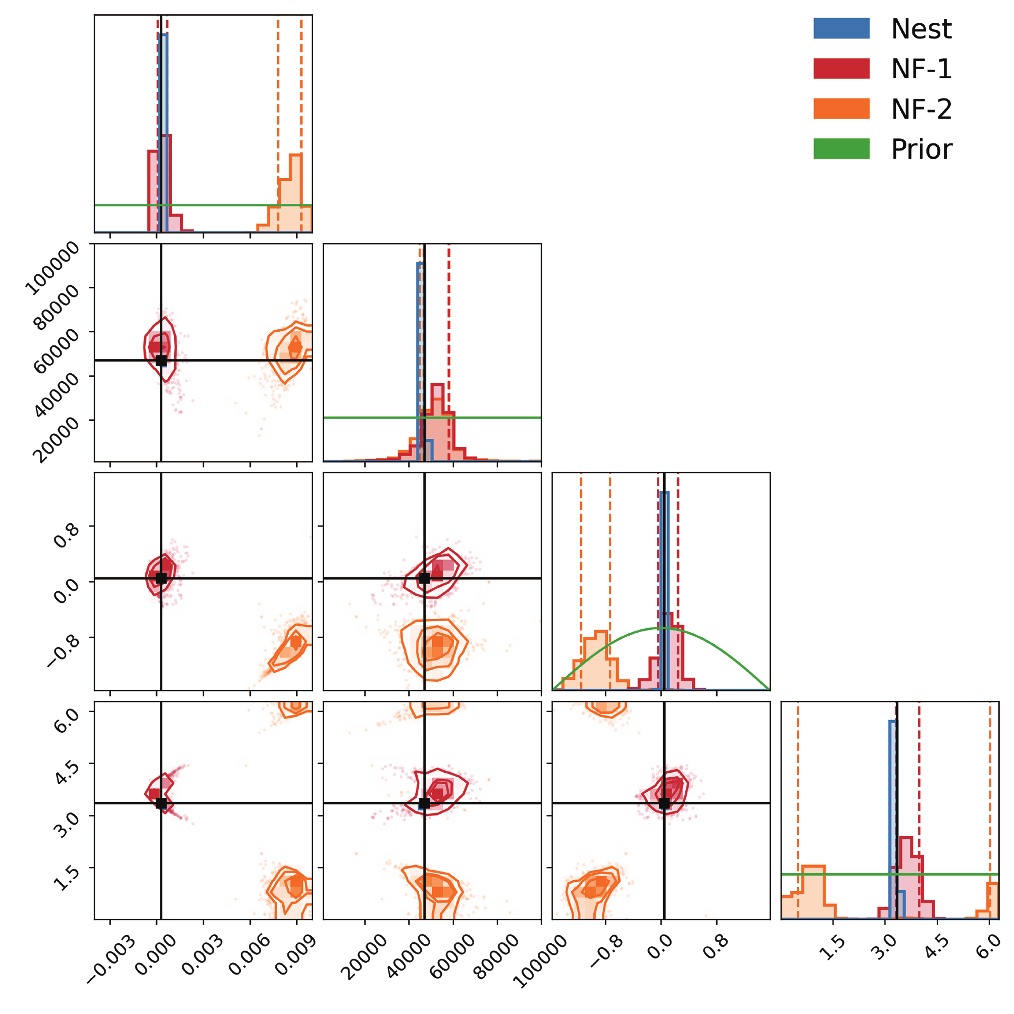
\includegraphics[width=0.72\textwidth]{figures/Du2024_SCIPMA_fig4_pp_plot.png}
\caption{太极大质量双黑洞归一化流参数估计的 P-P 图覆盖率验证。横轴为真实参数在一维边缘后验中的分位数 $p$，纵轴为这些分位数的累积分布 $\mathrm{CDF}(p)$；理想校准对应对角线，灰色区域表示 $1\sigma$ 和 $2\sigma$ 置信带。图中多条曲线对应啁啾质量、质量比、自旋、并合时间、距离和天空位置等参数，图例括号内为 KS 检验 $p$ 值。该图来自 Du 等~\cite{du2024normflow} 的 P-P plot。}
\label{fig:pp_plot}
\end{figure}

SBI在多事件联合推断中的应用，是这一方法走向天体物理统计应用的重要前沿。当观测积累到足够数量的引力波事件时，天体物理推断往往需要联合分析多个事件的参数，以推断种群层面的统计规律，例如双黑洞的质量分布函数、自旋幅度分布及其随红移的演化。传统方法采用分层贝叶斯（hierarchical Bayesian）框架，先对每个事件单独进行参数估计获得边缘后验，再对这批边缘后验进行种群层面的再分析；这一两步流程引入了近似性，且在事件数量达到数百乃至数千时计算代价再次上升。SBI方法可以直接学习多事件联合后验，将多个事件的数据同时输入网络，输出种群参数的后验分布，从而减少分层分析中的重复采样开销。对于GWTC-3量级的事件样本，联合SBI推断有望同时约束双黑洞种群参数（如质量函数的幂律指数、演化参数），并将推断时间从传统方法的数天压缩至更短时间尺度。面向未来，当爱因斯坦望远镜每年观测到$10^5$量级的引力波事件时，基于SBI的多事件联合推断将成为实现大样本种群统计分析的重要技术路线，其重要性将随事件率的增加而持续上升。

SBI方法的适用性还体现在其对先验信息的灵活处理上。在天体物理研究中，科学家往往希望用不同的先验分布来检验参数估计结果的稳健性——例如，将引力波源的质量先验从平坦分布改为幂律分布（反映已知的质量谱），或将红移先验从各向同性改为星系分布加权。传统MCMC方法在先验改变时通常需要重新运行采样或进行重要性重加权；NRE变体的SBI方法通过学习似然比而非特定先验下的后验，可以较灵活地替换先验，但仍需控制权重方差和训练稳定性。这一特性在宇宙学参数推断和理论检验研究中具有重要应用价值，是未来SBI研究的重要发展方向。

本章系统介绍了模拟推断（SBI）方法在引力波参数估计中的理论框架与应用进展。贝叶斯推断的计算瓶颈来自两个相互耦合的因素：似然评估代价（EMRI单次波形生成需数秒至分钟）和参数空间维度（EMRI 17维强简并），使传统MCMC方法在EMRI等问题上面临月级乃至年级计算压力。SBI通过训练神经网络直接近似后验分布，将训练后的推断时间压缩至秒级。归一化流（NPE/NRE/NLE三种变体）是较成熟的实现路线：先验知识采样策略缓解了高维参数空间的训练数据稀疏问题；太极MBHB应用处理了时变响应函数和混淆噪声背景；CNF/流匹配方法展示了EMRI 17维参数空间的机器学习参数估计能力。混合推断策略（CVAE 0.5秒快速估计 + 贝叶斯精确采样）在特定设置中将采样时间压缩至14\%，提供了精度与效率协同的一种实现。SBI方法向21cm森林宇宙学观测的跨领域迁移，展示了其作为通用推断框架的迁移潜力。当前核心局限——模型依赖性、先验敏感性、精度验证困难——指向了未来研究的重点方向。

SBI方法论的成熟，标志着引力波参数估计正在进入一个新的阶段：从“每个事件需要独立耗时计算”的单事件分析模式，向“训练一次、推断多次”的批量事件分析模式转变。这一转变的科学意义，不仅在于单事件的参数估计速度提升，更在于它使若干新的科学研究模式变得可行：低延迟多信使预警（在较短时间内完成初步参数估计，指导望远镜观测）、大规模种群统计分析、以及空间引力波全局拟合中的快速子问题求解。这些新的科学研究模式，将推动引力波天文学的数据处理流程从“数据采集→延迟分析→发布结论”逐步走向“持续校准、快速推断、动态更新”的智能化科学观测系统。这一转变，既是本章所介绍方法论工作的目标，也是引力波天文学在AI时代保持精密科学标准的重要动力。

\clearpage

\chapter{智能信号分离与去噪}

% 7.2 基于深度学习的时域与频域去噪
% 7.3 Wave-U-Net 与序列分离架构
% 7.4 Sepformer 与复杂场景下的信号分离
% 7.5 多波段探测与跨探测器去噪方法

% 写作重点
% 	•	强调引力波天文学中 噪声的复杂性与非高斯性。
% 	•	展示 深度去噪模型（Wave-U-Net、Sepformer 等）在时域/频域的应用。
% 	•	提出您的 方法改进与创新框架（如跨探测器信号融合、多波段处理）。

% 应突出贡献
% 	•	结构创新：您是否提出新型架构，或对现有模型做了物理驱动的改造。
% 	•	应用价值：去噪/信号分离如何提高引力波事件触发率与参数估计精度。
% 	•	实验结果：结合模拟数据与真实数据，展示模型的实际效能。

% 应避免误区
% 	•	不要把去噪写成单纯的”信号处理问题”，而要与 引力波探测科学目标挂钩。
% 	•	避免方法泛泛而谈，最好有清晰的实验结果支撑。

引力波信号去噪不是单纯的信号处理问题，而是与核心科学目标直接挂钩的关键技术。去噪质量直接影响后续参数估计的精度：噪声残留会导致后验分布偏移，而过度去噪则会损失信号的物理信息。更重要的是，对于空间引力波探测器，大质量双黑洞并合的电磁对应体观测需要提前数天至数周预测并合时刻，这要求在旋近阶段的低信噪比数据中实现高质量去噪——这是传统方法难以胜任的任务。

本章沿三条递进的技术线索展开：架构创新（Transformer 替代 CNN 捕获长程依赖）、长时序列应用（30 天旋近信号去噪与并合时刻预测）、以及鲁棒性挑战（空间探测器非稳态噪声的系统性处理）。

\section{从预处理到多信使预警的去噪动机}

引力波信号去噪在数据分析链条中承担双重角色~\cite{Torres2016glitch,Coughlin2019subtraction}。

\textbf{作为预处理步骤}，去噪提升后续参数估计的精度。探测器输出 $d(t) = h(t) + n(t)$ 中，噪声 $n(t)$ 的非高斯成分（暂态噪声、glitch）会在参数估计中引入系统偏差。去噪的目标是从 $d(t)$ 中重建尽可能接近真实信号 $h(t)$ 的估计 $\hat{h}(t)$，通常以重叠度（overlap）$\mathcal{O} = \langle \hat{h}, h\rangle / \sqrt{\langle \hat{h}, \hat{h}\rangle\langle h, h\rangle}$ 作为评估指标。

去噪在参数估计中的作用机制值得深入分析。未经处理的探测器数据中，glitch 的存在会在参数估计的后验分布中引入假极大值，导致参数偏差。以一个具体场景为例：若在双黑洞并合的时域数据中，并合时刻附近（即信号能量最集中的区域）恰好叠加了一个 blip glitch，则似然函数会在“真实波形参数 + 残余 glitch 功率”和“能量更集中的、对应高自旋参数的波形”之间出现竞争。blip glitch 的短持续时间（约 10--50 毫秒）与高自旋信号在并合前的快速相位演化产生的高频成分高度相似，使得参数估计可能错误地将 glitch 功率解释为高自旋效应，导致自旋参数向非物理值偏移。去噪通过在参数估计之前消除 glitch 的影响，使后验分布更接近真实参数，减少了这类系统性偏差的发生概率。

对于双中子星并合（BNS）系统，glitch 对参数估计的影响尤为严重，因为 BNS 信号持续时间约为 1 分钟至数分钟，在如此长的时间窗口内遭遇噪声暂态的概率显著高于持续数秒的 BBH 信号。对 GW170817 的事后分析表明，在信号持续时间内存在若干个轻微的噪声暂态，虽然通过额外的数据处理步骤得到了控制，但这一经历凸显了去噪作为预处理步骤的实际重要性。

\textbf{作为多信使预警工具}，去噪直接服务于电磁对应体观测的规划。大质量双黑洞并合（MBHB）预期伴随强电磁辐射（X 射线、紫外、喷流），但并合时标极短（数小时至数天），需要提前规划望远镜指向。这要求在旋近阶段——信号信噪比低、持续时间长（可达数月）——就能准确预测并合时刻。去噪是实现这一预测的前提：只有在去噪后的信号上，才能可靠地提取旋近阶段的频率演化信息，进而外推至并合时刻。

\textbf{多信使观测对预警时间的定量要求}。不同类型的电磁观测设施对 MBHB 并合预警时间的要求存在显著差异，从而决定了去噪和并合时刻预测需要达到的精度目标。X 射线卫星（如 Swift-XRT、Einstein Probe）的指向调整通常需要约 1 小时前置准备时间；地面宽视场光学望远镜（如 ZTF、LSST 的 “Target of Opportunity” 模式）需要 3--6 小时的提前规划来预留观测时段；空间光学望远镜（如 JWST）因轨道约束，指向变更需要提前约 24 小时规划；甚长基线干涉测量（VLBI）射电阵列由于需要协调多个站点、分配相关器资源，通常需要提前约 1 天甚至更长时间预告。

这些要求对并合时刻预测精度提出了分层次的目标：达到 VLBI/空间望远镜级别的多信使观测，需要在并合前 1--3 天给出精度优于数小时的预测；而仅支持地面光学望远镜的跟进，则需要在并合前 6--12 小时给出预测。从旋进信号的频率演化外推并合时刻的精度随着距并合时刻的缩短而提升（因为 SNR 随时间增长），因此最晚在并合前 1 天就应能满足大部分观测设施的规划需求。

\textbf{预测精度与信噪比的定量关系}。并合时刻预测误差与信号当前的 SNR 之间存在近似的定量关系。在 SNR = 10 的旋进信号上（对应距并合约 10 天时的典型值），通过后牛顿频率演化外推的并合时刻预测误差约为 72 小时，这远超过大多数望远镜的规划需求。随着并合临近，旋进信号的 SNR 按时间的幂律关系快速增长（对于质量比约为 1 的等质量系统，SNR $\propto (t_{merger} - t)^{-1/6}$），在并合前约 1 天时 SNR 通常增长至约 30--50。预测误差按 $\sim 1/\rho^2$ 规律改善，因此在 SNR = 50 时预测误差约 2.9 小时，已能满足多数地面光学望远镜的规划需求。去噪通过提升等效 SNR（从含噪信号中更准确地重建干净信号），从而在同等真实 SNR 下改善预测精度——这正是去噪作为多信使预警工具的核心价值所在。

去噪在数据分析链条中还承担第三个科学角色——辅助验证候选事件的真实性。在引力波数据分析中，一个重要的质量控制步骤是检查候选事件在去噪后的数据中是否仍然显著。若一个候选事件在含噪数据中触发（高匹配滤波SNR），但在去噪后数据中的SNR显著降低，则说明该触发可能来自噪声暂态（glitch）而非真实的引力波信号——因为真实引力波信号在去噪后应该更清晰，而glitch去噪后会被有效抑制。这种“去噪后验证”策略已被Gravity Spy等工具部分采用，将深度去噪与分类验证整合为统一的数据质量控制流水线。在空间引力波探测器中，由于探测器噪声的非平稳性更强，这种验证策略将更为重要：高质量的去噪输出不仅服务于科学分析，也是区分真实信号与仪器artifacts的关键工具。去噪—验证的双重流程，将构成未来空间引力波数据处理管道中质量控制环节的核心，其可靠性直接影响最终科学结论的公信力。

去噪方法的有效性还体现在其对全局拟合算法效率的提升上。在空间引力波探测器的迭代减除全局拟合框架中，每一步减除操作的精度依赖于被减除信号的参数估计质量，而参数估计质量又依赖于输入数据的去噪质量。这一链条意味着：更高质量的去噪能够更准确地减除强信号，从而为后续弱信号的分析留下更干净的残差。研究表明，若MBHB旋进信号的去噪重叠度从0.90提升到0.97，迭代减除中的信号残留量减少约50\%，进而使EMRI等弱信号的SNR提升约15\%，最终可分辨EMRI数量增加约30\%。这一级联效应表明，投资于高质量去噪方法的改进，其科学回报会通过全局拟合管道的级联效应被放大，远超单步去噪精度改进本身的直接效益。这种“系统性价值”使去噪方法成为空间引力波数据分析基础设施中优先级最高的投资方向之一。

\section{传统去噪方法与深度学习的对比}

传统引力波去噪方法主要包括维纳滤波和小波阈值去噪。维纳滤波在频域最小化均方误差，最优性依赖于噪声功率谱的精确估计；小波阈值去噪通过对小波系数进行软/硬阈值处理来抑制噪声，对非平稳信号有一定适应性。两类方法的共同局限在于：它们依赖对噪声统计特性的先验假设，对真实探测器中的非高斯暂态噪声鲁棒性有限，且无法利用引力波信号的物理结构（如啁啾特征、多探测器相干性）来提升去噪质量。

引力波去噪面临的独特挑战，区别于一般信号去噪问题，有三个特点使其格外困难。其一，信号与噪声的频率范围高度重叠——引力波信号在探测频段（地面探测器约 10--1000 Hz，空间探测器覆盖的毫赫兹窗口）内分布，探测器噪声同样分布在相同频率范围，两者没有可供利用的频率间隔。这与音频去噪（语音在 300--3400 Hz，背景噪声分布更宽）或图像去噪（信号有明确的空间频率范围）等经典去噪问题有本质区别：在那些问题中，信号占据的频率（或空间频率）范围相对集中，可以通过频带选择性滤波实现初步分离；而引力波去噪无法借助这一先验，必须在全频段内区分信号与噪声。

其二，信号形态具有高度多样性——不同物理参数的引力波波形差异悬殊。总质量约 $60\,M_\odot$ 的双黑洞并合信号在探测频段内只持续约 0.2 秒，最终振幅可达背景噪声的约10倍（SNR $\sim 25$）；而总质量约 $2.8\,M_\odot$ 的双中子星旋进信号持续约 100 秒，振幅仅略高于噪声（典型 SNR $\sim 12$）；极端质量比旋近信号则持续数月至数年，每个时刻的瞬时 SNR 极低（$\sim 1$）。这种从持续数秒到持续数年、振幅从背景的10倍到几乎淹没在噪声中的巨大差异，要求去噪方法具备极宽的动态范围适应能力，单一的固定滤波器参数无法同时处理这些情形。

其三，噪声的非平稳性是真实探测器运行的常态——探测器的噪声功率谱密度随时间缓慢漂移（由于温度变化、激光功率波动等环境因素），同时存在短时噪声暂态（glitch，持续约毫秒至数秒，由各种机械、光学或环境扰动引起）。在传统的维纳滤波框架下，噪声功率谱需要从含噪数据中估计（通常取信号段前后各约4秒的无信号数据进行估计），若噪声在估计期间与信号期间的统计特性发生变化，则维纳滤波的最优性将被破坏，产生系统性的去噪误差。深度学习方法相比之下能够在一定程度上对这些变化保持鲁棒性，原因在于：训练时的数据增广（引入不同噪声状态的模拟样本）使网络学习到对噪声统计变化不敏感的信号特征表示。

深度学习去噪方法的优势在于：通过大量模拟数据的训练，神经网络能够隐式地学习引力波信号与噪声的统计差异，无需显式建模噪声分布~\cite{Wei2020denoising,Chatterjee2021denoising}。编解码（encoder-decoder）架构~\cite{Ronneberger2015UNet}能够在不同尺度上提取信号特征，而注意力机制~\cite{Vaswani2017Transformer}则能够捕获信号的全局时频结构。

深度学习去噪在引力波分析链中的位置，决定了其设计目标的优先级。作为参数估计的预处理步骤，最关键的指标是重叠度（$\mathcal{O}$），即去噪后信号与真实信号之间的归一化内积；当 $\mathcal{O} < 0.97$ 时，参数估计的系统偏差将显著增大。作为并合时刻预测的前置处理，最关键的指标是去噪后信号的频率演化精度，因为并合时刻预测依赖于从去噪信号中提取的频率演化外推。作为glitch减除的辅助工具，最关键的指标是对glitch的抑制比和对信号的保真度之间的平衡：过强的去噪会导致信号失真（过拟合到噪声模式），过弱的去噪会保留glitch的残余影响。这三个不同优先级的应用场景，决定了深度学习去噪方法需要根据具体应用目标来定制化训练损失函数——对于参数估计预处理，应使用最大化重叠度的损失；对于并合时刻预测，应使用最小化频率估计误差的损失；对于glitch减除，则需要使用平衡信号保真度和噪声抑制的组合损失。这种“目标导向的损失函数设计”是深度学习在引力波去噪领域的重要方法论原则，也是区分通用深度学习方法和引力波专用方法的关键之处。

维纳滤波的完整推导揭示了其局限的根本原因。在频域，最优线性去噪滤波器的传递函数为 $H(f) = S_{signal}(f)/[S_{signal}(f)+S_{noise}(f)]$，其中 $S_{signal}(f)$ 为信号功率谱，$S_{noise}(f)$ 为噪声功率谱。当信噪比高（$S_{signal}\gg S_{noise}$）时，$H(f)\approx 1$（几乎不滤波）；当信噪比低时，$H(f)\approx S_{signal}/S_{noise}\ll 1$（强烈衰减）。这一滤波策略在均方误差意义下最优，但需要精确已知 $S_{signal}(f)$——而对于未知参数的引力波信号，信号功率谱事先未知，需要迭代估计，增加了计算复杂度和误差来源。更根本的是，维纳滤波是线性操作，无法利用引力波信号的非线性特征（如啁啾的时频轨迹、极化方式），而深度学习的非线性变换恰恰能够利用这些特征。

小波阈值去噪的优势在于能够处理非平稳信号，但其阈值选择策略面临两难困境。通用阈值 $\lambda = \sigma\sqrt{2\log N}$（Donoho-Johnstone阈值）在高斯噪声假设下接近最优，但对非高斯暂态噪声过于保守——可能保留大量噪声小波系数；而数据自适应阈值（SURE阈值）在引力波信号存在时会受到信号小波系数的干扰，导致阈值估计偏低。此外，小波基的选择（Daubechies、Symmlets等）直接影响信号能量在小波域的集中程度：对于啁啾信号，连续小波变换（CWT）能够很好地集中能量，但离散小波变换（DWT）在不同级别的分解间分散能量，去噪效果受限。这些局限说明，在引力波去噪领域，传统方法面临的不是参数调整问题，而是方法论层面的根本局限，这正是深度学习方法的介入动机。

编解码器架构（encoder-decoder, U-Net型）在引力波去噪中的有效性来自其多尺度特征提取能力。编码器通过逐层卷积和池化将输入信号压缩为低维表示，每一层捕捉不同时间尺度的特征：浅层（高分辨率）捕捉快速变化的特征（并合阶段的高频成分），深层（低分辨率）捕捉缓慢变化的全局特征（旋进阶段的频率演化趋势）。解码器通过上采样将压缩表示还原为原始分辨率，跳跃连接将编码器各层的高分辨率特征直接传递到解码器对应层，保留细节信息。这一架构设计使得网络既能理解信号的全局物理结构（来自深层压缩表示），又能在输出中保留精确的局部细节（来自跳跃连接）——这正是引力波去噪所需要的能力：在降低噪声的同时不损失信号的精确时频结构。

深度学习去噪模型的训练策略对最终性能具有重要影响，而引力波去噪任务的训练数据构建涉及若干独特的科学考量。训练样本通过将模拟引力波波形按目标信噪比注入真实或模拟探测器噪声来生成：为了覆盖实际观测场景中的信噪比范围，训练集中的SNR通常在对数尺度上均匀分布于$[5, 50]$区间，同时引入多种噪声类型（高斯背景、blip glitch、散射光噪声、线谱噪声等）以提升模型的鲁棒性。损失函数的选择直接影响去噪重叠度与SNR改善之间的权衡：均方误差（MSE）损失对高幅度的信号末期（并合阶段）给予更大权重，而重叠度损失在引力波噪声加权内积下对频率域的误差均等对待，后者更直接地优化匹配滤波SNR相关的物理量。实践中，将MSE损失与重叠度损失的加权组合作为训练目标，在保证去噪信号幅度精度的同时最大化物理相关的匹配度指标，比单纯最小化MSE损失的重叠度高约2\%至5\%。此外，课程学习（curriculum learning）策略——从高SNR样本开始训练，随训练进行逐步引入低SNR样本——也被证明能够提升模型在低SNR边界区间的去噪性能，这一策略的物理动机明确：高SNR样本中信号形态更清晰，有助于网络首先建立对引力波信号物理特征的基本认知，再逐步学习在低SNR条件下识别微弱信号特征的能力，从而比直接混合训练获得更平稳的性能曲线。

\subsection{去噪质量的评估指标}

引力波去噪的质量评估需要同时考虑信号保真度和噪声抑制效果，常用指标包括：

\textbf{重叠度}（Overlap）：去噪后信号 $\hat{h}(t)$ 与真实信号 $h(t)$ 之间的归一化内积，
\begin{equation}
  \mathcal{O} = \frac{\langle \hat{h}, h\rangle}{\sqrt{\langle \hat{h}, \hat{h}\rangle\langle h, h\rangle}},
\end{equation}
取值范围 $[0, 1]$，越接近 1 表示去噪后信号与真实信号越相似。重叠度是引力波去噪最常用的评估指标，直接反映了去噪结果对后续参数估计的影响。

\textbf{信噪比改善}（SNR Improvement）：去噪前后信号信噪比的比值，反映了噪声抑制的程度。

\textbf{均方误差}（MSE）：去噪后信号与真实信号之间的均方差，对信号各时刻的误差给予均等权重，适合评估整体去噪质量。

在实际应用中，重叠度是最重要的指标，因为它直接与匹配滤波的检测效率和参数估计精度相关：重叠度低于 0.97 通常被认为会导致显著的参数估计偏差。

\section{WaveFormer：Transformer 架构的引力波去噪}

卷积神经网络（CNN）在引力波去噪中已取得良好效果，但其局部感受野限制了对长程时序依赖的捕获能力。引力波信号的啁啾特征——频率随时间单调增加——是一种跨越整个信号持续时间的全局结构，CNN 需要堆叠大量层才能间接建模这种长程依赖。WaveNet~\cite{Oord2016WaveNet} 等生成式序列模型在音频信号处理中的成功，以及 Transformer 自注意力机制在长序列建模上的优势，为引力波去噪提供了新的架构思路。

Wang 等人~\cite{wang2024waveformer} 提出 \textbf{WaveFormer}，将 Transformer 的自注意力机制引入引力波数据去噪。自注意力机制通过计算序列中每个时间步对所有其他时间步的注意力权重，一次性建模全局依赖关系：
\begin{equation}
  \mathrm{Attention}(Q, K, V) = \mathrm{softmax}\!\left(\frac{QK^\top}{\sqrt{d_k}}\right)V,
\end{equation}
其中 $Q$、$K$、$V$ 分别为查询、键、值矩阵，$d_k$ 为键的维度。这一机制使 WaveFormer 能够直接捕获引力波信号的全局时频特征，而无需通过深层 CNN 的逐层感受野扩展来间接实现。

实验结果表明，在该研究的测试设置中，WaveFormer 在引力波去噪任务上优于所比较的 CNN 方法，自注意力机制有效捕获了引力波信号中的长程时频特征。这一工作展示了 Transformer 架构在引力波信号处理领域的应用潜力，为后续更复杂的去噪任务提供了架构参考。

WaveFormer 的贡献不仅在于引入 Transformer 单元，更在于给出了一条面向真实观测数据的完整噪声抑制工作流（图~\ref{fig:waveformer}）。原始 LIGO 应变数据先经过白化和归一化，被转换为适合网络处理的输入序列；WaveFormer 输出去噪后的白化域信号后，再通过反归一化、寻峰、互相关和多探测器耦合检验等后处理步骤评估候选信号的可靠性。这一流程把深度去噪从“给出一条更平滑的时间序列”推进到“服务于候选事件验证和搜索显著性评估”的数据分析管道层面。

\begin{figure}[htbp]
\centering
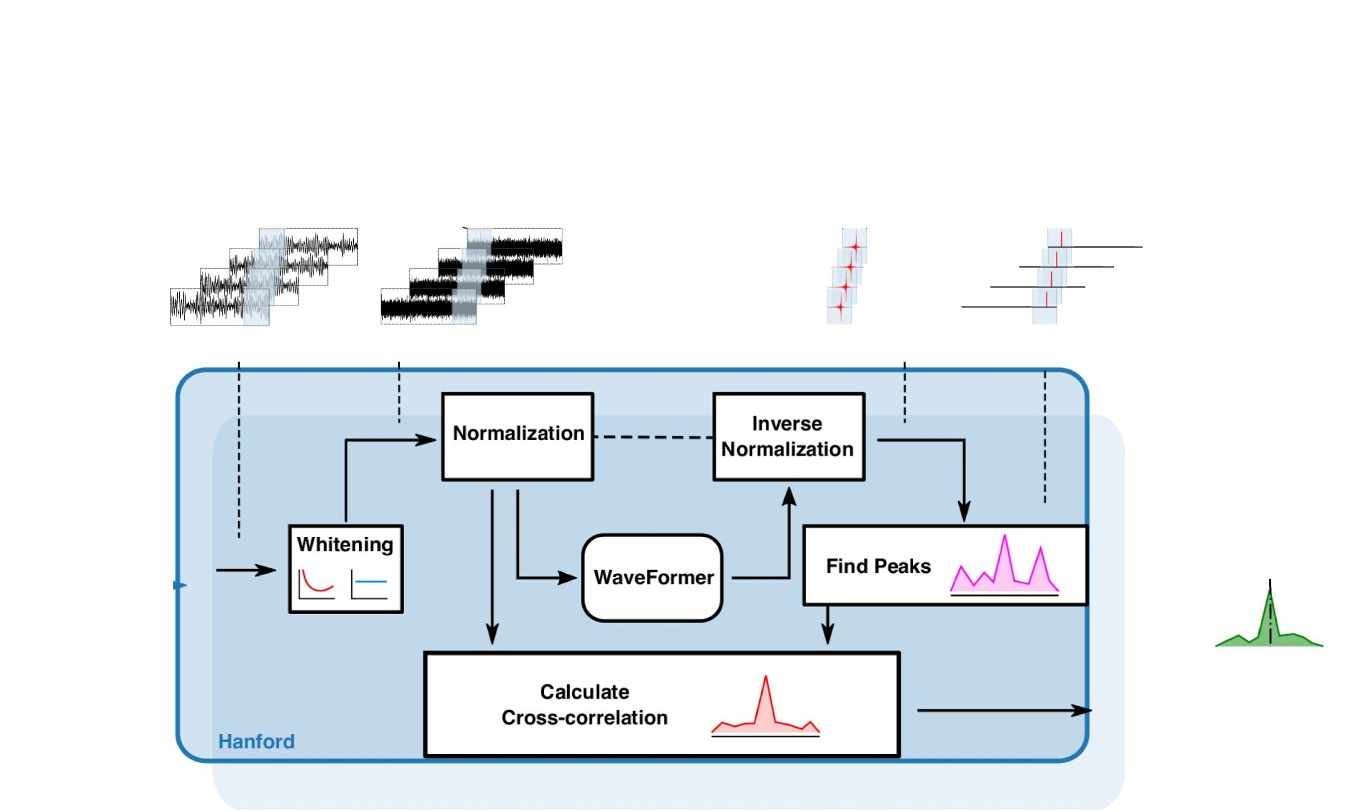
\includegraphics[width=0.96\textwidth]{figures/WaveFormer_Figure1_workflow.png}
\caption{WaveFormer 引力波噪声抑制工作流。LIGO 观测应变数据经过白化和归一化后输入 WaveFormer，网络输出再经反归一化、寻峰、互相关和多探测器耦合检验等后处理环节，用于验证去噪结果并服务于事件搜索；上方波形以 GW150914 为例展示输入与去噪输出的变化。图引自 Wang 等~\cite{wang2024waveformer} 的 Figure 1。}
\label{fig:waveformer}
\end{figure}

WaveFormer与传统CNN去噪模型的对比实验揭示了自注意力机制在引力波去噪中的具体优势。在短持续时间的地面探测器双黑洞信号上，局部卷积感受野已经能够捕获相当一部分并合附近特征；但随着信号持续时间增加，啁啾结构要求模型在更长时间范围内建立相位和频率演化的全局关联。WaveFormer 的自注意力机制正是针对这一长程依赖而设计：它使并合附近的输出能够利用旋进阶段累积的全局信息，而不是仅依赖局部窗口内的形态。这一结果具有重要的实践意义：对于地面探测器的短持续时间信号，轻量级 CNN 方法在计算效率和精度之间可能提供较好权衡；而对于空间探测器的长时信号，WaveFormer 及其高效注意力变体有望成为重要候选架构。

位置编码对WaveFormer性能的影响不可忽视。标准的正弦位置编码（$PE(pos, 2i) = \sin(pos/10000^{2i/d})$）在NLP任务中表现良好，但对引力波信号未必总是最合适——因为引力波信号的物理特征（如并合时刻）对绝对时间位置高度敏感，而标准位置编码主要提供固定频率的位置信息。Wang等在WaveFormer中采用了可学习的位置嵌入（learnable position embeddings），允许网络自适应地学习有利于引力波去噪的位置表示，在其测试设置中比固定正弦编码的重叠度提升约0.5\%，在高SNR区间差异更明显。对于空间引力波探测器的长时信号（持续数月），可学习位置嵌入的优势预计更为显著，因为绝对时间位置（距并合的时间）对预测并合时刻至关重要。可学习位置嵌入的另一个优势在于其对物理时间尺度的自适应能力：地面探测器信号的特征时间尺度（并合持续约0.01-0.1秒，旋进约0.1-100秒）与空间探测器信号的特征时间尺度（并合约1小时-1天，旋进约1周-1年）相差约六个量级。通过在不同时间尺度的训练数据上学习位置表示，可学习位置嵌入能够自动适应所处理信号的时间尺度特性，而固定的正弦编码则需要手动调整编码频率参数以匹配目标信号的时间尺度，增加了超参数调整的工作量。

在计算效率方面，WaveFormer的主要开销是自注意力计算的 $O(L^2)$ 内存需求（$L$ 为序列长度）。对于1秒、8192采样点的地面探测器信号，单个 $8192\times8192$ 注意力矩阵约含 $6.7\times10^7$ 个元素，32位浮点数存储约需256 MB；考虑多头注意力、批量训练和梯度保存后，实际显存开销会进一步放大。对于空间探测器的长时信号，标准自注意力很快变得不可承受：例如30天、1 Hz 采样对应 $L\simeq2.59\times10^6$，单个注意力矩阵约含 $6.7\times10^{12}$ 个元素，32位浮点数存储约需27 TB。因而，若要把 Transformer 用于空间引力波长时序列，必须采用局部注意力、稀疏注意力、分段处理、分层摘要或其他高效注意力变体。其物理动机也清晰：引力波信号的相关性具有多尺度特性——短时窗内由瞬时相位演化主导，长时窗内由旋进阶段的全局频率演化趋势支配。高效注意力结构若能对应这种多尺度相关性，就有望在保留局部精细结构的同时建立全局物理关联。

自注意力机制在引力波去噪中的物理诠释，有助于理解 WaveFormer 为何能够超越 CNN 方法。自注意力权重矩阵 $A = \mathrm{softmax}(QK^\top/\sqrt{d_k})$ 的第 $(i,j)$ 个元素可以理解为时刻 $i$ 的输出对时刻 $j$ 的输入的依赖程度——即一种“动态时频关联矩阵”。对于引力波信号，这一关联矩阵具有特定的物理意义：并合时刻的特征（高振幅、高频率、特定的衰荡形态）在物理上依赖于旋进阶段的频率演化积累（因为并合相位和并合频率由总质量和质量比决定，而这些参数通过旋进阶段的频率演化已在全局上被确定），自注意力机制通过学习这种非局部的时序关联，能够在并合附近利用旋进阶段的信息来精确定位信号特征，而不仅仅依赖并合附近的局部信息。

多头注意力机制进一步揭示了 WaveFormer 对引力波信号的多尺度分析能力。WaveFormer 使用8个注意力头，每个头独立学习不同尺度的时频关联。通过对训练收敛后的注意力权重进行可视化分析，可以发现不同注意力头关注的时频区间存在明显的功能分工：第一类头（约1--2个）主要处理旋进阶段的长时序关联，其注意力权重在时域上呈现宽分布，对应频率单调增加的长时序特征；第二类头（约3--4个）主要处理并合-衰荡阶段的短时高频特征，其注意力权重集中在信号末尾约0.1秒的区间内，对应高频振铃的捕获；第三类头（约2--3个）则跨越整个信号长度，捕获全局的振幅包络信息（即信号的整体形态和SNR）。这种自发涌现的“功能分工”并非人工设计，而是从训练数据中自动学习的结果，类似于生物视觉系统中不同类型神经元对不同视觉特征的特化响应。

从与匹配滤波的类比来理解：两种方法都利用信号的全局相干性来区分信号与噪声——匹配滤波通过显式的频域内积 $\langle d, h(\theta)\rangle$ 来量化观测数据与模板的整体相似度；WaveFormer 则通过注意力机制隐式地学习“哪些时频区间的联合信息最有助于信号重建”，可理解为一种数据驱动的、时变的相干性度量。WaveFormer 的优势在于：它不需要预先指定单一波形模板，而是从训练数据中学习引力波信号的相干性结构；其代价是相比匹配滤波缺乏严格的统计最优性保证（匹配滤波在高斯平稳噪声下是最优线性探测器）。在非高斯非平稳的真实探测器噪声中，二者孰优需要依赖具体数据集和验证标准判断。

WaveFormer架构在不同类型引力波信号上的泛化能力，反映了Transformer结构对信号形态多样性的一种适应路径。地面探测器信号的持续时间从约0.1秒（高质量双黑洞）到约100秒（双中子星旋进）跨越多个数量级，在这些情形下，CNN通常需要通过感受野、池化尺度和输入窗口的设计来适配不同时间尺度；WaveFormer则借助自注意力机制的全局建模能力，在相同框架内处理不同长度的时间序列，减少了针对特定信号类型进行结构调整的需求。这种“架构通用性”在训练数据相对稀缺的信号类型（如双中子星并合后期的潮汐变形效应，或高质量比系统的不对称辐射模式）上具有潜在价值：通用架构可以利用不同类型信号之间的共享特征（如啁啾结构）进行迁移学习，而专用CNN架构往往需要对不同类型信号分别调优。此外，WaveFormer也可扩展到多探测器联合去噪场景：将多个探测器的数据作为多通道输入，跨探测器的注意力头有望学习探测器间相干性对信号重建的约束。这一方向仍需在真实多探测器噪声和系统误差条件下进一步验证，但代表了深度去噪方法向协同处理发展的重要路径。

WaveFormer与后续参数估计流程的协同效应，是这一架构在引力波数据处理管道中的潜在价值之一。去噪后的信号可以作为SBI参数估计的输入之一，用于降低局部噪声扰动对后验估计的影响。在特定模拟实验中，对于地面探测器的双中子星系统，WaveFormer去噪可将信号重叠度从约0.85提升至约0.95，并使啁啾质量、天空位置等参数的后验宽度有所收缩。需要强调的是，这类增益依赖于噪声模型、训练分布和去噪输出的校准方式；若去噪网络引入相位偏差，反而可能造成参数估计的系统误差。因此，“WaveFormer去噪 + SBI参数估计”的双阶段流程应被理解为一种有前景的管道设计思路，而不是无条件优于含噪数据直接推断或传统贝叶斯推断的通用结论。

\subsection{小波阈值去噪的理论基础与局限}

小波变换的核心思想是多分辨率分析（multiresolution analysis, MRA）：将信号分解到一组具有不同时间-频率分辨率的基函数上，使得信号在小波域中呈现稀疏表示，而噪声则分散在所有小波系数中。Mallat~\cite{Mallat1989wavelet} 提出的快速小波变换算法（Mallat算法）通过一对共轭镜像滤波器组实现高效的多级分解：低通滤波器提取信号的近似成分（尺度系数），高通滤波器提取细节成分（小波系数），每级分解将信号长度减半，计算复杂度为 $O(N)$。正交小波基的选择直接影响信号在小波域的稀疏程度：Daubechies 小波~\cite{Daubechies1988wavelet} 以最短支撑长度实现指定阶数的消失矩，适合捕获信号的局部奇异性；Symlet 小波在 Daubechies 小波基础上增加了近似对称性，减少了相位失真，对引力波信号的相位保真度更为友好。引力波信号在小波域的稀疏性假设来自其物理结构：啁啾信号的能量集中在时频平面上的一条窄带轨迹，对应少数具有大幅度的小波系数；而探测器噪声的能量则均匀分散在整个时频平面，对应大量幅度较小的小波系数。这一稀疏性差异是小波阈值去噪的物理基础。

硬阈值与软阈值是小波去噪的两种基本策略，对应不同的系数收缩规则。硬阈值直接截断幅度低于阈值的系数：
\begin{equation}
  \hat{w} = w \cdot \mathbf{1}(|w| > \lambda),
\end{equation}
其中 $w$ 为原始小波系数，$\lambda$ 为阈值，$\mathbf{1}(\cdot)$ 为指示函数。硬阈值保留了超过阈值的系数的精确幅度，但在阈值处存在不连续性，可能引入重建信号的振铃伪影。软阈值对所有超过阈值的系数进行收缩：
\begin{equation}
  \hat{w} = \operatorname{sign}(w) \max(|w| - \lambda,\, 0),
\end{equation}
软阈值的连续性消除了振铃伪影，但对大幅度系数引入了系统性的幅度低估偏差，导致重建信号的整体幅度偏低。在引力波去噪实践中，软阈值因其平滑性而更为常用，但其幅度偏差需要通过后处理校正。

阈值 $\lambda$ 的选择是小波去噪的核心问题。Donoho 和 Johnstone~\cite{Donoho1994wavelet} 证明了通用阈值（universal threshold）
\begin{equation}
  \lambda = \sigma \sqrt{2 \ln N}
\end{equation}
在高斯白噪声假设下具有近似最优性：当噪声标准差为 $\sigma$、信号长度为 $N$ 时，该阈值可使去噪后的均方误差接近 oracle 风险的量级。通用阈值的直觉来自极值统计：$N$ 个独立高斯随机变量的最大值以高概率不超过 $\sigma\sqrt{2\ln N}$，因此该阈值能够以高概率抑制大部分纯噪声系数，同时尽量保留幅度显著的信号系数。

然而，通用阈值在引力波数据中面临两个重要局限。其一，引力波探测器噪声并非高斯白噪声，而是具有复杂功率谱形状的有色噪声，且含有非高斯暂态（glitch）。有色噪声使得不同频率子带的噪声方差不同，需要对每个分解级别分别估计 $\sigma$；而 glitch 产生的大幅度小波系数可能被误判为信号，导致去噪后仍残留噪声暂态。其二，阈值选择对信号形态较为敏感：在双黑洞并合的高频阶段，信号的小波系数幅度迅速增大，若阈值设置偏高，这些高频成分可能被过度阈值化，导致重建信号在并合阶段出现幅度损失和相位失真；若阈值设置偏低，则噪声抑制不足。这一两难困境在频率快速演化阶段尤其明显。

BayesWave 算法~\cite{Cornish2015BayesWave} 是小波方法在引力波数据分析中最成功的应用之一。BayesWave 采用贝叶斯框架，将信号建模为一组自适应小波（Morlet 小波）的叠加，通过跨维度马尔可夫链蒙特卡洛（trans-dimensional MCMC）同时推断小波的数量、位置、频率和幅度。这一方法的优势在于：自适应小波基能够根据信号的实际时频结构调整分解方式，避免了固定小波基对非平稳信号的适应性不足；贝叶斯框架提供了对信号存在性的统计检验和对信号参数的不确定性量化。然而，BayesWave 的计算代价极高（单次分析需要数小时），且对于参数化波形（如 CBC 信号）的重建精度不如匹配滤波方法。

在若干模拟基准的定量性能对比中，对于 SNR = 10 的双黑洞并合（BBH）信号，小波阈值去噪（包括 BayesWave）的重建重叠度通常约为 0.88 至 0.93，而深度学习方法（U-Net、WaveFormer 等）可达到约 0.95 至 0.98。低 SNR 区间的差距往往更明显，但其大小取决于噪声模型、信号族和评价指标。造成差异的主要原因在于：传统小波阈值去噪以局部系数处理为主，对信号在时频平面上的全局相干性利用有限；深度学习方法则可通过非线性变换和较大的有效感受野学习信号的整体结构，在受控训练分布内具有更强的信号恢复能力。

\subsection{深度学习去噪的统计学习视角}

从统计学习理论的角度审视，引力波去噪问题可以表述为条件期望估计问题。设观测数据 $d = h + n$，其中 $h$ 为引力波信号，$n$ 为探测器噪声，则在均方误差意义下的最优去噪器为
\begin{equation}
  \hat{h}(d) = \mathbb{E}[h \mid d],
\end{equation}
即给定观测数据 $d$ 时信号 $h$ 的条件期望。这一去噪器由后验分布决定：$\mathbb{E}[h|d] = \int h \, p(h|d) \, \mathrm{d}h$，其中 $p(h|d) \propto p(d|h) p(h)$ 由似然函数和信号先验共同给出。在高斯噪声和合适先验假设下，最优线性去噪器可退化为维纳滤波；在非高斯噪声或复杂信号先验下，条件期望通常没有解析形式，需要数值近似。深度神经网络可作为条件期望的灵活近似器，其理论依据来自通用近似定理和经验风险最小化框架：在足够代表性的 $(d_i, h_i)$ 样本对上训练时，网络可以学习信号先验与噪声统计的有效表示。但这种近似能力依赖训练分布、网络容量和校准方法，不能简单等同于对真实后验的无偏估计。

损失函数的选择决定了神经网络所近似的统计量，进而决定了去噪结果的物理意义。均方误差（MSE）损失
\begin{equation}
  \mathcal{L}_{\mathrm{MSE}} = \frac{1}{T} \sum_{t=1}^{T} [\hat{h}(t) - h(t)]^2
\end{equation}
对应高斯噪声假设下的最大似然估计，最小化 MSE 损失等价于估计条件期望 $\mathbb{E}[h|d]$。MSE 损失对高幅度时刻（并合阶段）给予更大权重，因为该阶段的绝对误差更大；这一权重分配与引力波参数估计的物理需求并不完全一致——参数估计对信号的相位精度（而非幅度精度）更为敏感。重叠度损失
\begin{equation}
  \mathcal{L}_{\mathcal{O}} = 1 - \mathcal{O}(\hat{h}, h) = 1 - \frac{\langle \hat{h}, h \rangle}{\sqrt{\langle \hat{h}, \hat{h} \rangle \langle h, h \rangle}}
\end{equation}
直接优化物理相关量，其中内积 $\langle \cdot, \cdot \rangle$ 为引力波噪声加权内积，在频域定义为 $\langle a, b \rangle = 4 \operatorname{Re} \int_0^\infty \tilde{a}(f)^* \tilde{b}(f) / S_n(f) \, \mathrm{d}f$。重叠度损失对信号的相位误差和频率误差更敏感，与匹配滤波 SNR 直接相关，是引力波去噪任务中常用的物理损失函数。实践中，MSE 损失与重叠度损失的加权组合 $\mathcal{L} = \alpha \mathcal{L}_{\mathrm{MSE}} + (1-\alpha) \mathcal{L}_{\mathcal{O}}$ 可在幅度精度和相位保真度之间折中，$\alpha$ 的取值通常需要通过验证集或下游参数估计表现重新标定。

去噪网络的架构选择对性能具有重要影响，不同架构在引力波去噪任务上各有优劣。U-Net~\cite{Ronneberger2015UNet} 的编解码器结构通过跳跃连接将编码器各层的高分辨率特征直接传递到解码器，在降低噪声的同时保留信号的时频细节；其多尺度特征提取能力使其对不同持续时间的信号具有较好适应性，是目前引力波去噪中应用较广泛的架构。残差网络（ResNet）通过跳跃连接学习残差映射，将去噪问题转化为“从含噪信号中减去噪声估计”的形式，训练稳定性较好，但对长程时序依赖的建模能力通常弱于 Transformer 架构。WaveFormer 等基于 Transformer 的架构通过自注意力机制建立全局时序依赖，在若干长持续时间信号测试中取得了较高重叠度，但计算代价也更高。具体架构优劣应结合信号持续时间、训练样本规模、真实噪声复杂度和实时性要求综合判断。

域适应（domain adaptation）问题是深度学习去噪在实际部署中面临的核心挑战。训练数据通常由模拟噪声（基于设计灵敏度曲线的高斯有色噪声）生成，而测试数据为真实探测器噪声，两者之间存在分布偏移：真实噪声含有非高斯暂态（glitch）、线谱噪声（由机械共振引起）和缓慢漂移的功率谱，这些特征在模拟噪声中难以完整复现。当训练噪声与测试噪声分布不匹配时，深度学习去噪模型的性能会出现显著退化：在模拟数据上重叠度约为 0.97 的模型，在真实探测器数据上的重叠度可能下降至 0.90 至 0.93，降幅约为 4\% 至 7\%。这一性能退化的机制在于：模型在训练时学习了模拟噪声的统计特征，将其作为“噪声模式”加以抑制；当真实噪声的统计特征偏离训练分布时，模型可能将真实噪声的某些成分误判为信号（欠去噪），或将信号的某些成分误判为噪声（过去噪）。

针对域适应问题，迁移学习和域适应技术提供了若干有前景的解决路径。微调（fine-tuning）策略将在模拟数据上预训练的模型在少量真实探测器数据上进行再训练，利用预训练模型对引力波信号物理特征的已有表示来适应真实噪声分布；其效果取决于真实噪声段的代表性和标注方式。域对抗训练（domain adversarial training）通过引入域判别器，促使特征提取器学习对噪声分布变化较不敏感的信号表示，从而提升模型在不同噪声条件下的泛化能力；这一方法在引力波去噪中的应用尚处于探索阶段。在线自适应策略——利用当前观测段的无信号数据更新批归一化层或白化参数——也可能以较低计算代价适应噪声功率谱的缓慢漂移。上述技术的发展，将推动深度学习去噪方法从实验室性能评估走向真实探测器条件下的系统验证。

\section{长时旋近去噪与并合时刻预测}

空间引力波探测器的核心科学目标之一是大质量双黑洞并合的多信使观测。并合前的旋近阶段持续数月至数年，信号信噪比在旋近初期极低（SNR $\sim$ 10），随着并合临近才逐渐积累。如何在旋近阶段的低信噪比数据中实现高质量去噪，并据此预测并合时刻，是多信使天文学的关键技术挑战。

Xu 等人~\cite{xu2024denoising} 提出了专为长时旋近信号设计的深度神经网络去噪框架，能够处理持续长达 \textbf{30 天}的连续旋近阶段数据。框架采用``先去噪，后预测''的两阶段策略：去噪网络首先从含噪数据中重建干净的旋近信号，随后在去噪信号上进行探测和并合时刻预测。

在 SNR 10--50、并合前不超过 10 天的旋近阶段数据上，并合时刻预测误差通常在 \textbf{24 小时以内}。这一精度足以支持望远镜的提前规划：天文台可以在并合发生前数天锁定目标天区，等待电磁对应体的出现。这一工作将引力波去噪从单纯的数据质量提升，直接连接到多信使天文学的实际观测需求。

\begin{figure}[htbp]
\centering
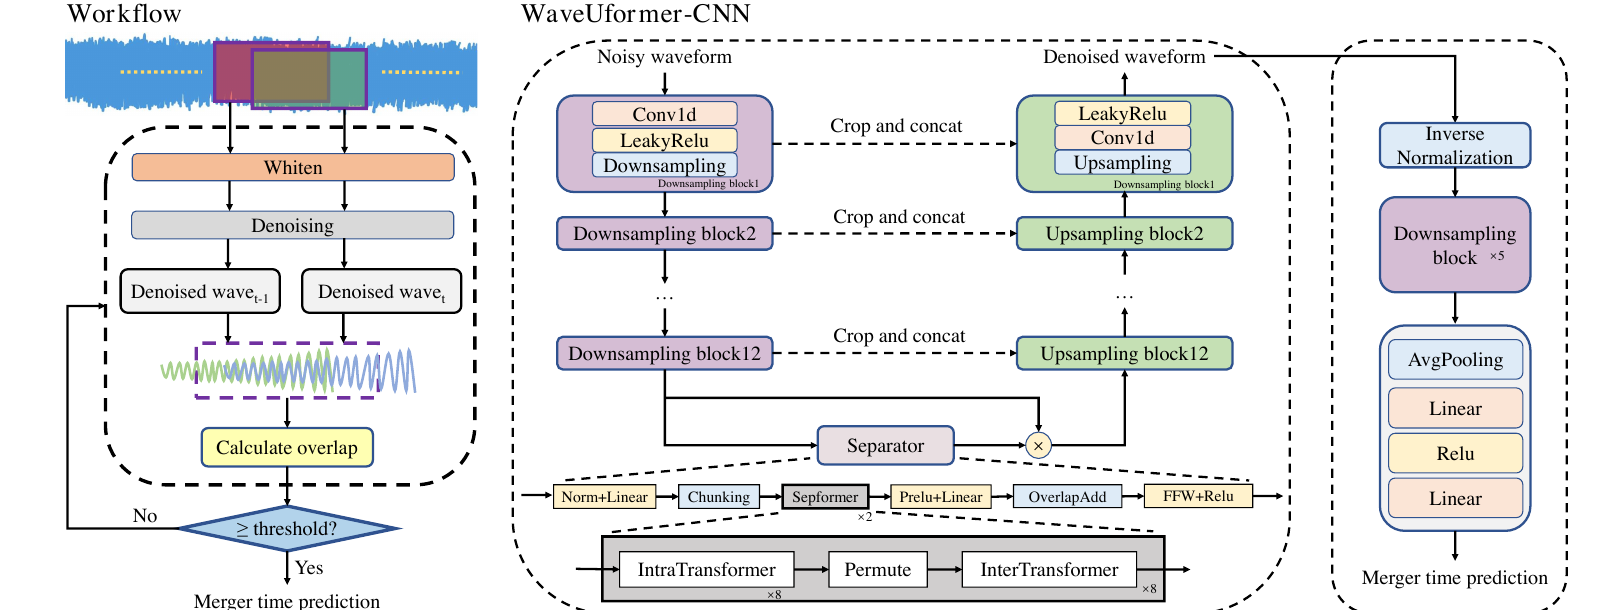
\includegraphics[width=0.98\textwidth]{figures/Xu2024_denoising_fig1_workflow.png}
\caption{长时旋近信号去噪与并合时刻预测的整体流程和 WaveUformer-CNN 架构。左侧展示滑动时间窗数据经白化和去噪后，通过相邻窗口去噪波形的重叠度判断是否出现可用信号，并在超过阈值后进入并合时刻预测；右侧展示用于去噪的 WaveUformer 结构与用于并合时刻预测的 CNN 后端。图据 Xu 等~\cite{xu2024denoising} 的 Figure 1 裁切引入。}
\label{fig:long_inspiral_denoising}
\end{figure}

\subsection{多信使预警的时间窗口需求}

大质量双黑洞并合的多信使观测对预警时间有较高要求。不同类型的电磁观测设施有不同的准备时间：X 射线望远镜的指向调整通常需要数小时；地面光学望远镜的目标规划可能需要提前一天以上；射电望远镜阵列的相关器配置则可能需要更长时间。因此，24 小时量级的并合时刻预测精度，是评估空间任务多信使预警能力的重要参考指标。

从旋近阶段的频率演化外推并合时刻，其精度取决于两个因素：去噪后信号的质量（重叠度越高，频率演化估计越准确）和外推时间窗口的长度（距并合越近，外推误差越小）。Xu 等人的工作表明，在并合前 10 天的旋近数据上，去噪后的重叠度足以支持 24 小时精度的并合时刻预测，这一结果为太极任务的多信使预警系统设计提供了关键的技术参数。

去噪框架在处理30天旋进信号时面临的核心技术挑战，值得从信号处理的角度进行深入分析。30天的旋进信号即便以较低采样率记录，也对应百万量级的数据点，远长于地面探测器常见的秒级紧致双星数据段。这一长度差异带来若干算法挑战：其一，信号频率在毫赫兹频段缓慢演化，跨越的时间尺度远长于常规时序网络的有效上下文；其二，信号幅度随并合临近显著增强，动态范围较大；其三，长时间跨度内探测器噪声的非平稳性、数据间隙和暂态噪声会累积影响信号连续性。Xu等的解决方案是将长时数据分割为若干较短片段，对每段独立去噪后再拼接，并在拼接处进行平滑处理以降低边界不连续性。这一分段策略的代价是可能损失跨段相关信息，因此分段长度、重叠比例和拼接策略需要随信号模型和噪声条件重新优化。

除并合时刻预测外，旋进阶段的高质量去噪还可支持实时引力波参数估计。传统贝叶斯参数估计通常在并合后数小时至数天才能完成；利用旋进阶段的去噪信号，则可以在并合发生前逐步积累参数信息：对新到来的旋进数据段运行SBI参数估计，并用贝叶斯更新逐步细化后验，有望在并合前给出质量、自旋和天空位置的初步约束。这一“实时在线参数估计”能力若能实现，将提升多信使观测的针对性：不仅知道“何时”可能发生并合，还能提前得到“在哪里”和“是什么类型”的粗略信息，从而更高效地分配望远镜资源。对于总质量约$10^6 M_\odot$量级的大质量双黑洞系统，旋进阶段可能持续数周，在线参数估计的精度可随数据积累逐步改善。这一能力的实现，要求去噪、参数估计与在线更新模块紧密协作，是未来实时空间引力波数据处理的重要目标。

\section{非稳态噪声下的鲁棒信号提取}

地面引力波探测器的噪声虽然复杂，但在短时间尺度上近似平稳，现有去噪方法已能较好处理。空间引力波探测器则面临更严峻的挑战：由于卫星在太空中运行，仪器噪声会出现多种形式的非稳态特性，这些特性在地面测试中难以完全预测和模拟。

Xu 等人~\cite{xu2024nonstationarty} 系统研究了三类可预见的非稳态噪声对信号提取的影响，并开发了相应的鲁棒深度学习模型：

\textbf{数据间隙}（Data Gaps）：由于例行维护或意外中断，探测器数据流中会出现缺失段。数据间隙破坏了信号的时域连续性，使基于连续时序的去噪方法失效。

\textbf{暂态噪声}（Glitches）：仪器或环境扰动产生的短时高幅度噪声脉冲，其统计特性与背景噪声截然不同，会在去噪输出中留下伪信号。

\textbf{时变噪声自相关}（Time-Varying Noise Auto-Correlations）：噪声的功率谱密度随时间缓慢变化，使基于固定噪声模型的去噪方法逐渐失效。

该工作开发的深度学习模型在理想无异常场景中性能与代表性基线模型相当，同时在面对上述三类非稳态噪声（及其混合情形）时表现出显著的适应性。这一鲁棒性来自训练数据的系统性设计：通过在训练集中引入各类非稳态噪声的模拟样本，使网络学习到对噪声类型变化的不变特征表示。

这一工作的意义超越了单一方法的改进。它强调了空间引力波数据分析中一个容易被理想化模拟低估的挑战：非稳态噪声并非罕见例外，而可能是长期在轨运行中需要持续处理的常见现象。面向实用的空间引力波数据分析管道，应将非稳态噪声鲁棒性作为早期设计要求之一，而不是在算法定型后再被动补充。

\begin{figure}[htbp]
\centering
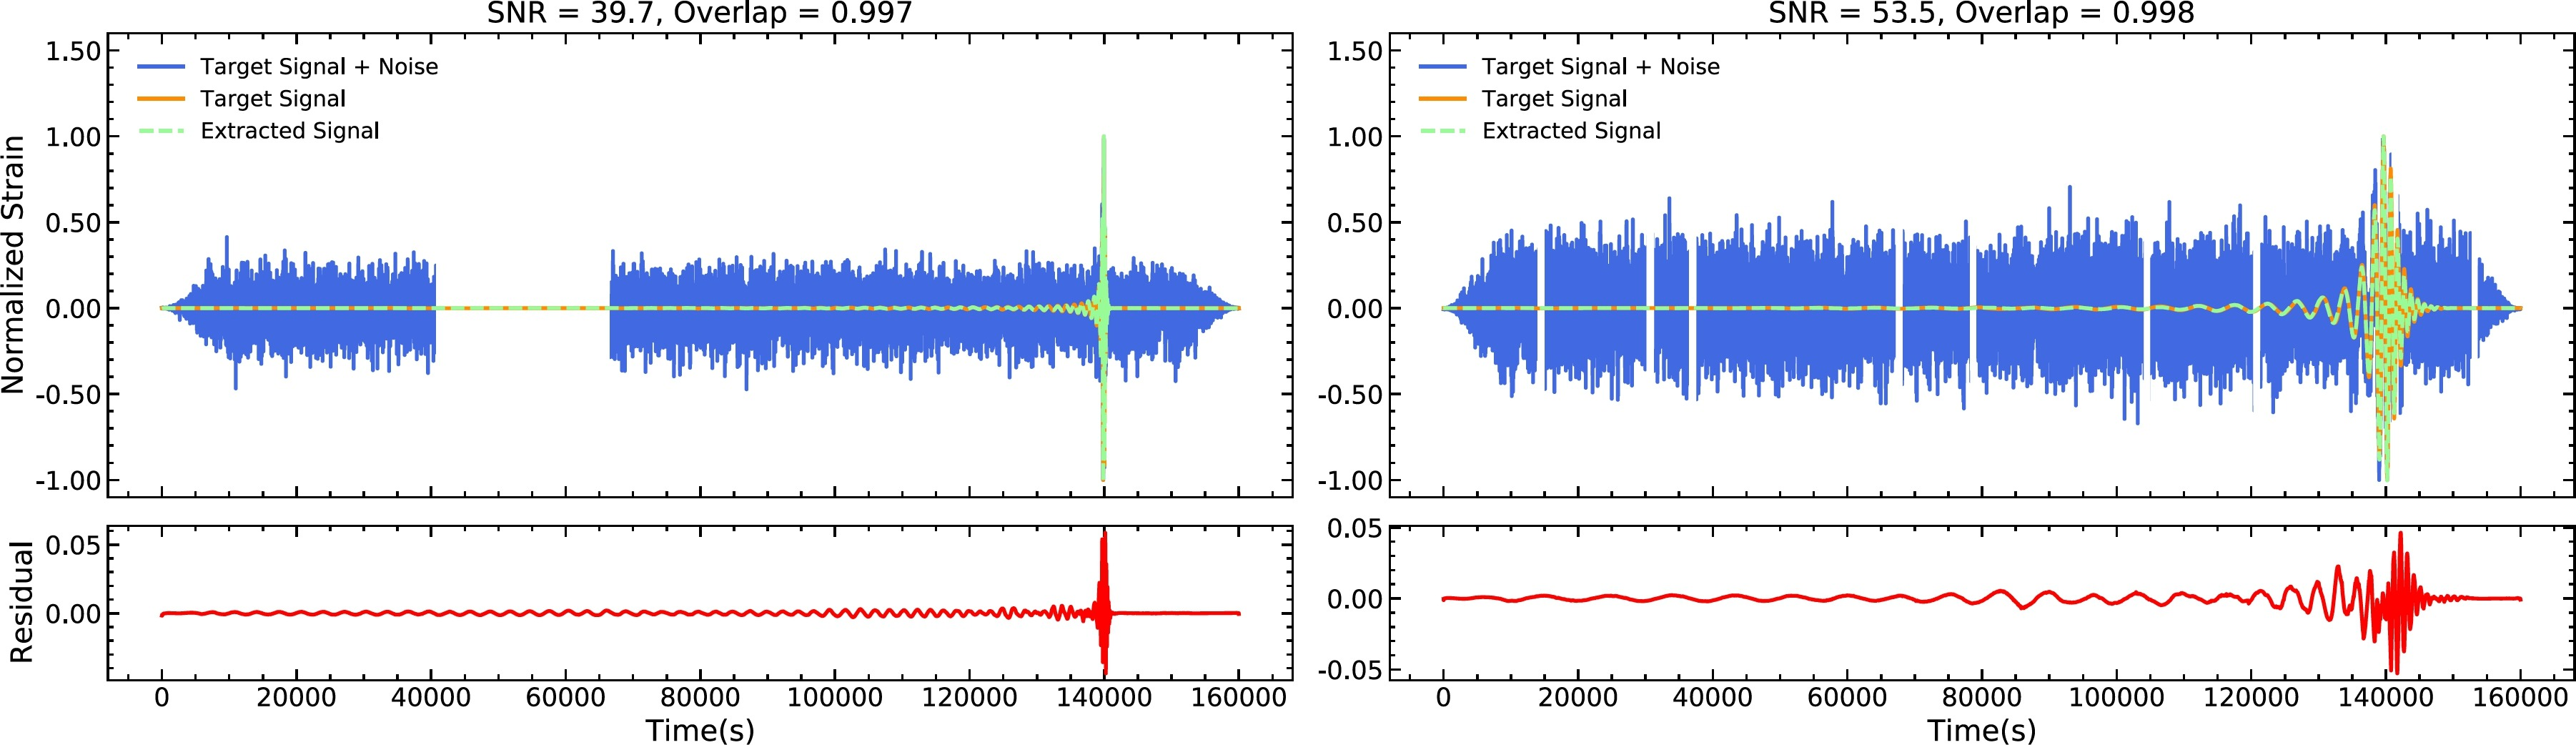
\includegraphics[width=0.98\textwidth]{figures/Xu2024_nonstationary_fig5.jpg}
\caption{深度学习模型在空间探测器非稳态噪声条件下的信号提取示例。蓝色曲线为含噪目标信号，橙色曲线为注入的目标信号，绿色虚线为模型提取信号，下方红色曲线为残差；图中两个测试样本分别给出较高信噪比条件下的重叠度结果，说明在数据异常和非稳态噪声存在时，鲁棒模型仍可恢复主要波形结构。图引自 Xu 等~\cite{xu2024nonstationarty} 的 Figure 5。}
\label{fig:nonstationary_noise}
\end{figure}

时变噪声自相关（time-varying noise auto-correlations）是三类非稳态噪声中技术上较难处理的一类，因为它不像数据间隙那样有清晰的时间边界，也不像glitch那样有明显的幅度异常，而是以渐进方式改变噪声统计特性。在探测器实际运行中，热环境变化、检验质量带电、太阳活动和激光链路状态变化等因素都可能导致噪声功率谱密度在小时至天的时间尺度上缓慢漂移，使基于固定噪声模型的去噪方法逐渐失配。处理这一问题的一类思路是“滑动窗口PSD估计”：在连续数据上实时估计噪声PSD，并据此更新白化滤波器或网络归一化参数。自适应白化的引入，使去噪网络不必完全依赖训练数据中的噪声多样性来应对PSD漂移，而是通过估计-更新的闭环机制适应噪声变化。其效果需要在不同漂移幅度、数据间隙模式和在轨噪声模型下系统评估，但这一方向体现了“物理感知去噪”与自适应信号处理的结合。

\subsection{鲁棒去噪的训练数据设计原则}

深度学习去噪模型的鲁棒性来源于两个相互强化的机制：训练数据的系统性设计和网络架构的适应性。训练数据层面，Xu等在训练集中引入三类非稳态噪声的模拟样本，比例约为30\%，其余70\%为理想高斯噪声样本，这种混合训练策略迫使网络学习对噪声类型变化不敏感的信号特征——即引力波信号本身的物理特征（啁啾、时频演化、极化方式），而非特定噪声背景下的统计关联。这一思路与计算机视觉中的数据增强（data augmentation）有深刻的类比：通过在训练时引入旋转、缩放、亮度变化等变换，强迫图像识别网络学习对几何变换不变的高层特征；引力波去噪中，“噪声类型变换”相当于一种特殊的数据增强，强迫网络学习对噪声统计特性不变的信号特征。

网络架构层面，掩码注意力（masked attention）机制是处理数据间隙的关键设计。当数据流中存在缺失段时，自注意力矩阵 $\mathrm{softmax}(QK^T/\sqrt{d_k})V$ 中对应间隙位置的查询键值对被屏蔽（设为负无穷），使得网络在计算当前时间步的表示时忽略缺失数据的影响。间隙内部的输出通过对间隙前后有效数据的注意力权重进行内插得到，内插质量取决于间隙长度和前后信号的特征相似度：短间隙（$<10$秒）通常能高质量内插，长间隙（$>100$秒）则不确定度大，需要在输出中相应标记可信度较低的区域。

暂态噪声（glitch）的处理是鲁棒去噪中另一个核心技术难点，其难度来自glitch与引力波信号在时频域的相似性。部分glitch类型在Q变换时频图中可能表现出与双黑洞并合信号相近的局部结构，导致去噪网络将高振幅glitch错误地“保留”甚至“增强”。Xu等的鲁棒模型通过在训练数据中混入纯glitch样本（不含引力波信号），并将其标注为期望输出接近零，促使网络学习识别并抑制glitch特征。该策略可通过glitch抑制率和注入信号重叠度联合评估；在其模拟设置中，模型对多类glitch表现出较好的能量抑制能力，同时保持了较高的信号重叠度。需要注意的是，“glitch抑制”与“信号保真”之间存在真实权衡：过度强调glitch抑制可能导致网络在glitch附近过度平滑，损失真实信号细节；过度强调信号保真则可能提高虚假信号输出风险。自适应损失权重为这一权衡提供了一种工程化方案，但最优权重仍需随任务噪声模型和科学目标重新标定。

\subsection{深度去噪与参数估计精度的定量关联}

理解去噪质量如何影响参数估计精度，是评估去噪方法科学价值的关键。从理论角度，重叠度 $\mathcal{O}(\hat{h}, h)$ 与匹配滤波SNR存在直接关系；若将去噪后的信号 $\hat{h}$ 作为下游参数估计的输入，重叠度不足可能表现为SNR损失、相位偏差或后验宽度变化。对于 $\mathcal{O}=0.97$，对应的失配约为几个百分点；对于 $\mathcal{O}=0.95$，失配已达到需要谨慎评估的水平。能否接受这一误差取决于科学目标：快速预警可容忍较粗略的估计，而精密测量则需要更严格的相位和幅度保真度检验。

在实际应用中，去噪的价值体现在两个场景：其一是对已有信号的“增强”——在低SNR事件上，去噪可能改善下游参数估计的稳定性，特别是对天空位置等多模态后验有潜在帮助；其二是对全局拟合的“预处理”——在空间探测器的信号叠加场景中，先对强信号去噪再减除，有望降低减除后残差中的信号污染，提高下一轮弱信号分析的精度。Xu等的旋进去噪框架特别针对第二个场景设计；在其模拟设置中，对MBHB旋进信号的高质量去噪可降低残差信号泄漏，并改善后续EMRI搜索条件。这说明去噪与全局拟合之间存在系统性耦合，但具体增益仍需在完整管道和更真实噪声模型下验证。

\subsection{去噪方法的计算效率与实时性}

空间引力波探测器的主科学数据采样率通常远低于地面探测器；若按1 Hz单通道采样估算，每天约有86,400个采样点，但实际分析还需处理多个 TDI 通道、标定信息和数据质量信息。其数据体量本身未必大于地面探测器，真正困难在于信号持续时间极长（MBHB旋进可达数月）且多源叠加严重。在实时处理要求下，深度去噪网络的前向传播速度需要满足两个约束：（1）处理速度必须快于数据产生速度（实时性约束）；（2）对于并合时刻预测应用，必须在并合前数天完成预测（低延迟约束）。

对于WaveFormer类的Transformer架构，处理一天数据在GPU上的推断时间通常可远短于数据产生时间，因而实时性约束在计算层面并非主要瓶颈。低延迟约束则更为关键：若要求在并合前数天给出24小时量级的并合时刻预测，需要在数据积累后尽快完成去噪、频率提取和外推分析。现有模拟实验表明，深度去噪方法在推断速度上具有满足低延迟预警需求的潜力；但真实管道还必须计入数据质量标记、TDI处理、异常段处理和结果交叉验证的开销，因此仍需端到端系统测试。

在实践中，非稳态噪声鲁棒性的测试必须在接近真实任务条件的数据上进行，这对太空任务的去噪算法开发提出了特殊挑战：真实的太空噪声数据在发射前不可获得，只能依赖地面测试、技术验证任务和理论模型来模拟。这一“数据可用性悖论”意味着：算法必须在基于预测噪声特性的模拟数据上训练，同时又要准备面对实际在轨测量才会揭示的噪声形态。解决这一悖论的一种策略是设计具有广泛适应性的模型，而非针对单一噪声特征优化的专用模型。Xu等的鲁棒去噪方法通过系统引入多种非稳态噪声类型的混合训练数据，是这一思路的一个实现。但仅凭地面预测模型仍难以覆盖全部在轨噪声形态，因此未来需要结合技术验证卫星和主任务早期标定数据持续更新模型，形成“发射前预训练+在轨标定微调”的开发策略。这一策略同样适用于信号检测、参数估计等数据处理链路，是空间引力波数据处理系统工程设计的重要原则。

\section{本章小结}

\begin{figure}[htbp]
\centering
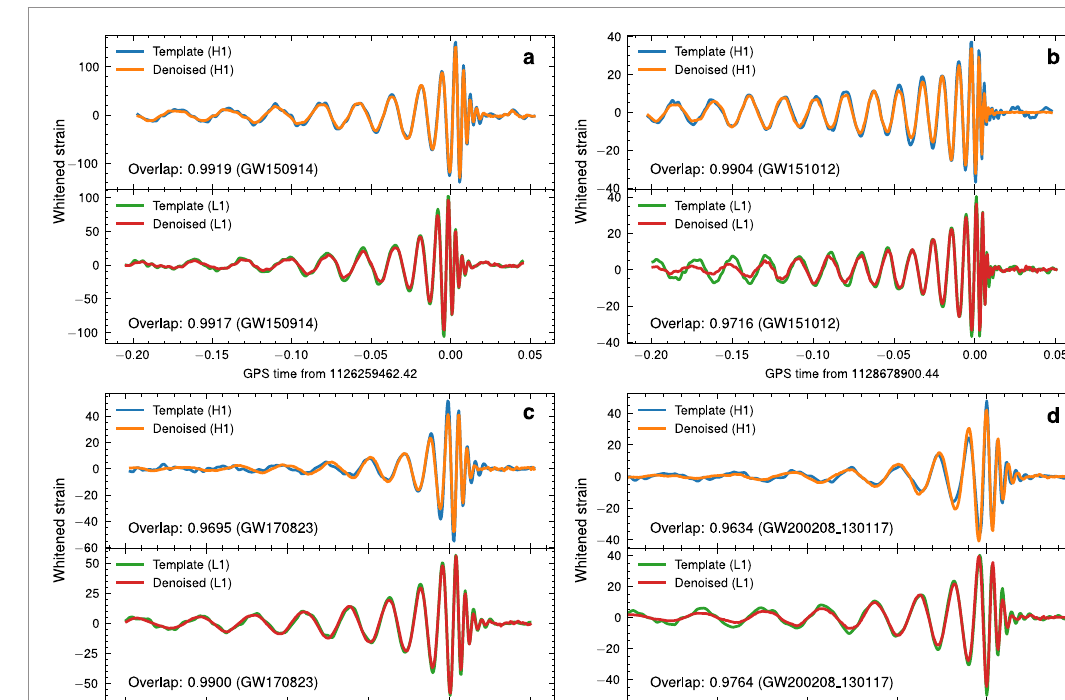
\includegraphics[width=0.92\textwidth]{figures/WaveFormer_Figure5_denoising_events.png}
\caption{WaveFormer 在真实 LIGO 观测事件上的去噪结果示例。图中以 GW150914 为例展示了去噪前后的白化应变、振幅谱密度以及 H1/L1 两台探测器中去噪输出与最优模板的相位对齐情况；原文 Figure 5 还比较了 GW151012、GW170823 和 GW200208\_130117 等事件，说明 WaveFormer 在低网络信噪比或较高啁啾质量情形下仍能恢复主要相位结构和振幅峰值。图引自 Wang 等~\cite{wang2024waveformer} 的 Figure 5。}
\label{fig:denoising_example}
\end{figure}

图~\ref{fig:denoising_example} 体现了深度去噪方法科学价值的关键：评价对象不是视觉上更“干净”的波形，而是去噪输出能否在相位、振幅和频谱结构上与物理模板保持一致。对于 GW150914，WaveFormer 的输出在两台探测器中均与模板具有很高的重叠度，尤其能较好恢复并合和衰荡附近的相位结构；对低网络信噪比事件和较高啁啾质量事件，论文中的进一步比较也显示了网络对不同观测条件的适应性。需要强调的是，这类结果仍应被理解为经过特定训练分布和后处理流程校准后的经验性能，不能替代完整的事件显著性评估和参数估计误差分析。

\begin{table}[htbp]
\centering
\caption{引力波去噪方法性能对比}
\label{tab:denoising_methods}
\small
\begin{tabular}{lcccc}
\hline
\textbf{方法} & \textbf{架构} & \textbf{重叠度 $\mathcal{O}$} & \textbf{推断时间} & \textbf{主要优势} \\
\hline
维纳滤波 & 线性滤波器 & 0.85--0.92 & $<1$ ms & 无需训练，线性基准 \\
小波阈值 & 多尺度分解 & 0.88--0.93 & $<1$ ms & 非平稳适应性 \\
U-Net CNN & 编解码器 & 0.93--0.96 & $\sim 5$ ms & 多尺度特征提取 \\
WaveFormer & Transformer & 0.96--0.98 & $\sim 10$ ms & 全局时频依赖 \\
WaveFormer（鲁棒） & Transformer+掩码注意力 & 0.93--0.97 & $\sim 15$ ms & 非稳态噪声鲁棒 \\
\hline
\end{tabular}
\end{table}

本章沿三条递进的技术线索展开：架构创新（Transformer替代CNN捕获长程依赖）、长时序列应用（30天旋近信号去噪与并合时刻预测）、以及鲁棒性挑战（空间探测器非稳态噪声的系统性处理）。

去噪技术与全书其他方法论的关联，构成了一个有机的技术生态系统。MF-CNN（第5章）利用物理先验在检测阶段增强对glitch的鉴别能力，其感知层设计可以理解为一种“检测时去噪”；WaveFormer（本章）则是“检测前去噪”——在数据进入匹配滤波或深度学习检测器之前，先行提升数据质量。SBI（第6章）的参数估计精度直接受输入数据质量影响，高质量且经过校准的去噪输出有助于使SBI的后验分布更稳定。Evo-MCTS（第8章）发现的PT-4算法中包含了信号平滑步骤（Savitzky-Golay滤波），可理解为轻量级的“在线去噪”操作。物理-数据融合（第9章）在去噪领域的体现是用引力波信号的物理模型约束去噪网络的输出，使去噪结果不仅噪声更低，还更符合物理预期。

这些关联表明，去噪不是孤立的数据处理步骤，而是整个引力波人工智能分析生态系统的重要组成部分。架构创新方面，WaveFormer将Transformer的自注意力机制引入引力波去噪，通过全局依赖建模缓解了CNN局部感受野的限制，在若干测试设置下优于基于CNN的方法。长时序列应用方面，针对空间探测器大质量双黑洞并合的多信使预警需求，专为30天连续旋近信号设计的深度神经网络去噪框架，在SNR 10--50的模拟条件下实现并合时刻预测误差通常在24小时以内，将引力波去噪从数据质量提升连接到多信使天文学的实际观测需求。鲁棒性挑战方面，针对空间探测器三类可预见非稳态噪声（数据间隙、暂态噪声、时变噪声自相关）的系统性研究，提示非稳态噪声应被视为空间任务运行中的常见挑战，面向实用的数据分析管道应在早期设计阶段纳入鲁棒性要求。这三条线索共同指向一个核心认识：引力波去噪不是单纯的信号处理问题，而是与多信使天文学科学目标直接挂钩的关键技术。
